\chapter{Analysis}
\label{ch:Analysis}



This section analyzes the results of the collected data from the first and second studies. For both studies, we begin by analyzing the participant data, followed by an assessment of how the participants perceived the different tests in terms of difficulty, using the NASA-TLX and questions related to the comparison of the setups. Specifically, we focus on which setup participants found to be better. Next, we examine the actual performance results to compare perceived performance with actual performance.

To describe the Braille-dot components, we represent the keys using their respective numbers within a dot, as shown here: \textcircled{i} for character $i$, similar to the figures presented previously.

\subsection{First Study}

\begin{table}
\resizebox{\columnwidth}{!}{
    \centering
    \begin{tabular}{|c|c|c|c|} \hline 
        Gender & Age & Dominant Hand & Previous Braille Knowledge\\ \hline 
        M & 27 & R & No\\ \hline 
        M & 27 & R & No\\ \hline 
        M & 22 & R & No\\ \hline 
        M & 22 & R & No\\ \hline 
        M & 26 & R & No\\ \hline 
        M & 27 & R & No\\ \hline 
        M & 28 & R & No\\ \hline 
        W & 28 & R & No\\ \hline 
        W & 27 & R & No\\ \hline 
        M & 30 & L & No\\ \hline 
        M & 25 & R & No\\ \hline 
        W & 55 & R & No\\ \hline
    \end{tabular}}
    \caption{General participant data in the first study.}
    \label{tab:study1_participant_data}
\end{table}
\begin{figure}
    \centering
    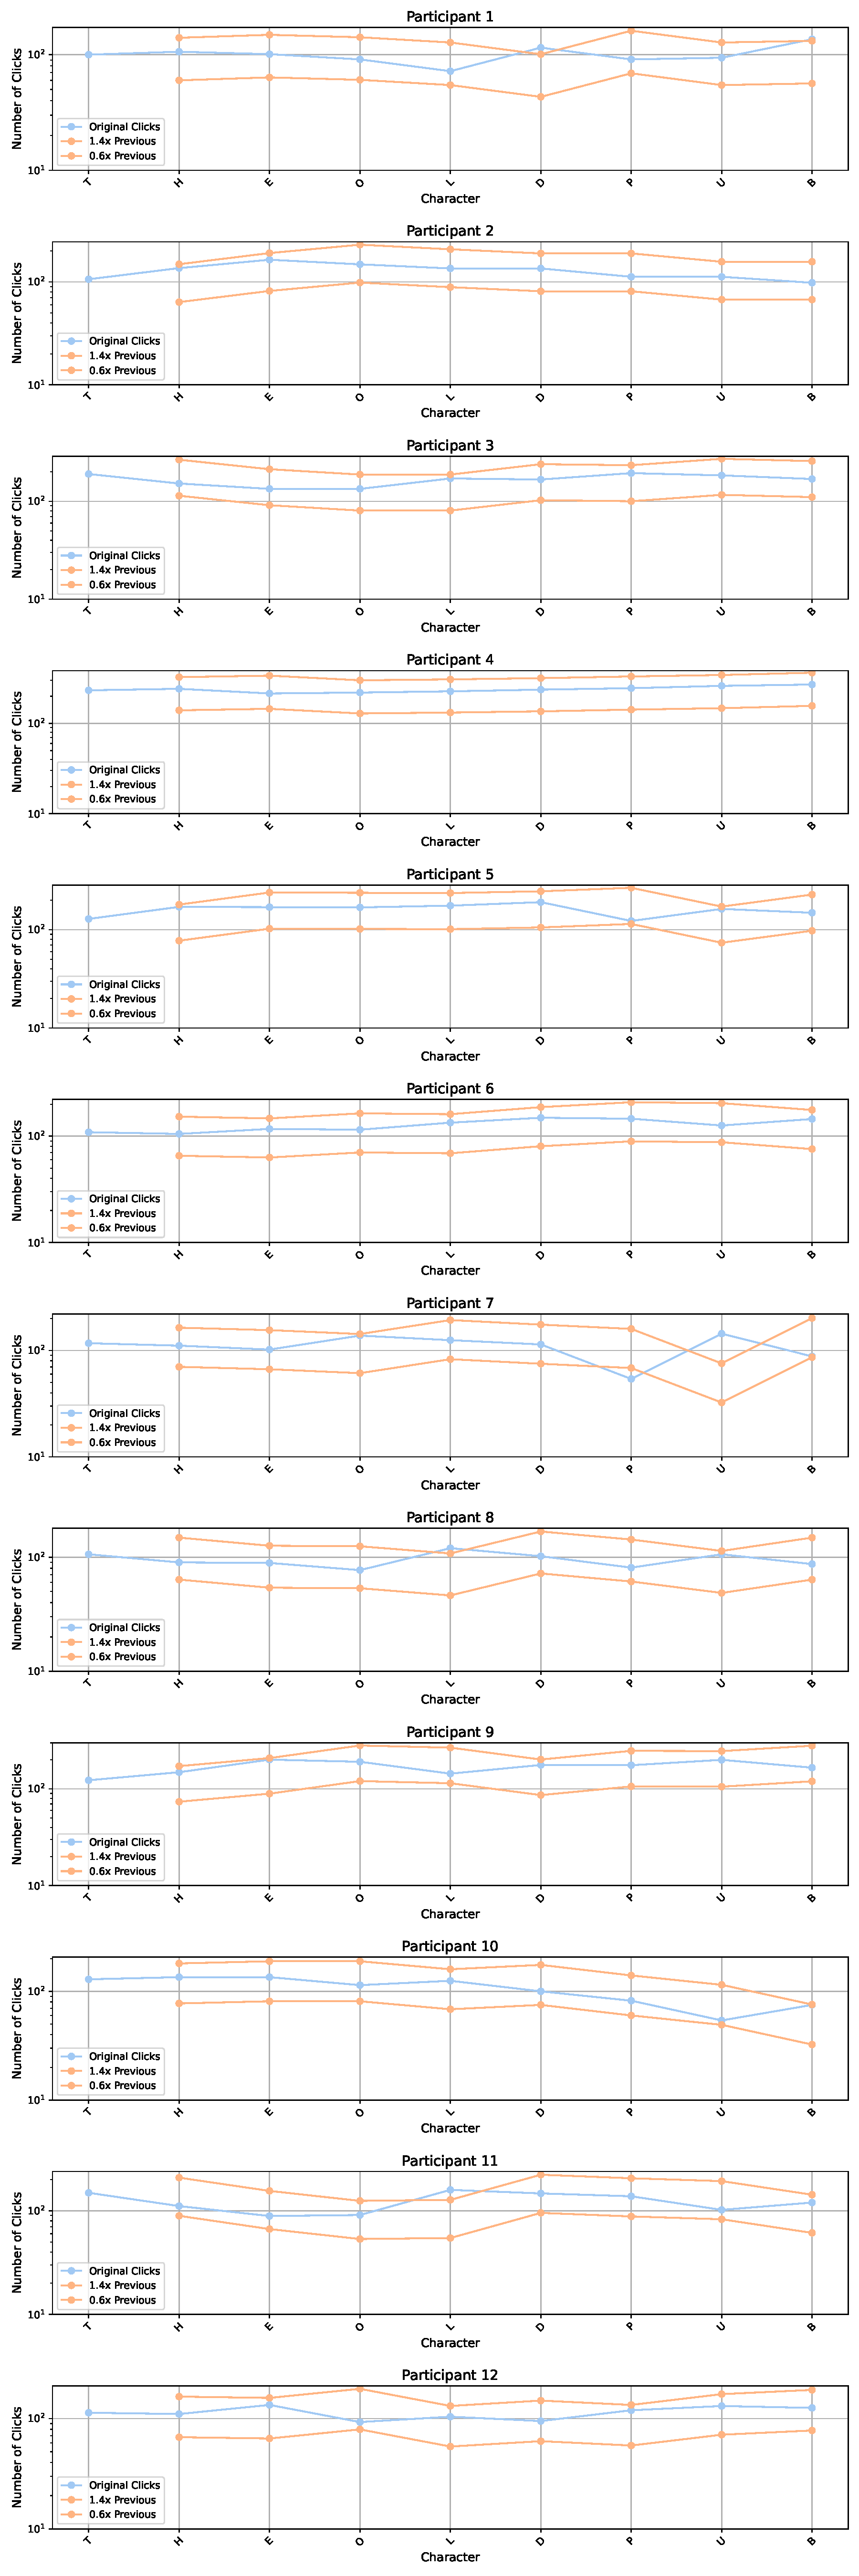
\includegraphics[width=0.5\linewidth]{src/pictures/Study1Data_questionnaire/participantPlots_study1.pdf}
    \caption{Participant Click-differences.}
    \label{fig:participant_clicks-firstStudy}
\end{figure}

In the first study, we interviewed 12 participants (3 female, 9 male), aged between 22 and 55, with an average age of 28.67 and a median age of 27 years. Of these, 11 were right-handed, and one was left-handed, as shown in \autoref{tab:study1_participant_data}. None of the participants had prior knowledge of Braille.

First, we assessed the validity of our data by ensuring that the participants were focused on the game and not on the sensations themselves. To do so, we measured the click rate for each character to detect any differences in performance. Given that participants tended to become more fatigued later in the game, we compared the click rates with those from the previous round to determine whether the data showed a 40\% improvement or decline, as indicated by the two red lines in \autoref{fig:participant_clicks-firstStudy}. As shown, the data passed the test, with the exception of participant 7, where the observed difference can be attributed to the stimulus change and the completion of questionnaires between sessions.


\begin{figure}
    \centering
    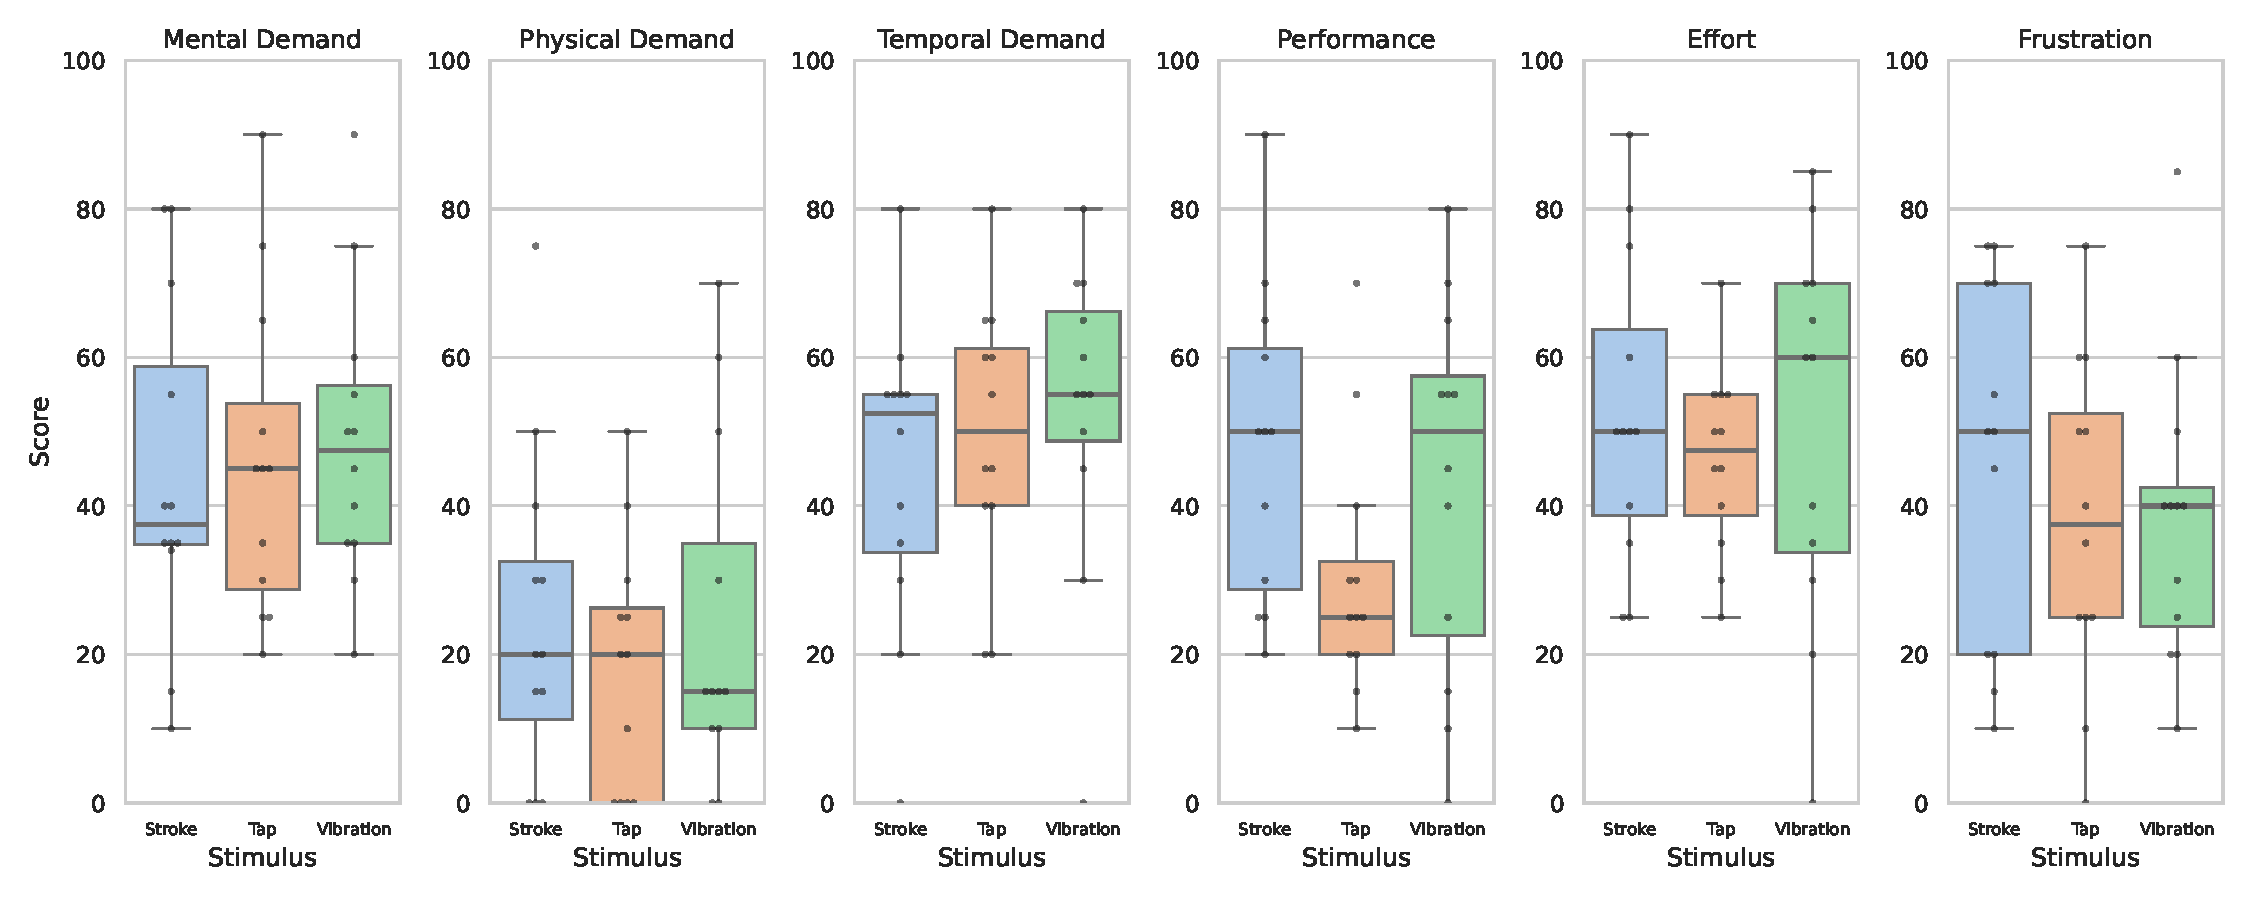
\includegraphics[width=\linewidth]{src/pictures/Study1Data_questionnaire/NasaTLX_study1.pdf}
    \caption{Raw Nasa TLX scores for the different Stimuli grouped by the Nasa TLX dimensions.\\ Each dot represents one participant.}
    \label{fig:nasaTLX-firstStudy}
\end{figure}

The raw NASA-TLX scores are presented in \autoref{fig:nasaTLX-firstStudy}, which displays boxplots for the different stimuli and their corresponding NASA-TLX scores, grouped by the respective NASA-TLX dimensions.

Overall, the medians for the dimensions are similar, with the most notable difference observed in the "performance" dimension. Specifically, the medians are 25.0 for tapping, 50.0 for stroking, and 50.0 for vibration.

In the "physical demand" dimension, a noticeable difference in the quantiles is apparent. The quantile for tapping is slightly larger, indicating that it performed worse on average. Similarly, in the "effort" dimension, slight differences in the quantiles and medians are observed. The medians for stroking and tapping are 50 and 47.5, respectively, while the median for vibration is 60.

In the "frustration" dimension, the quantile range is larger, particularly for the boxplot representing stroking, which has a quantile range of Q1 = 20, Q3 = 70, with a median of 50. In contrast, tapping has a Q1 of 25, Q3 of 55, and a median of 37.5. Vibration shows the smallest quantile range, with a Q1 of 23.5, Q3 of 42.5, and a median of 40.

Subsequently, we tested for significant differences between the sets using Kruskal-Wallis significance tests, the results of which are tabulated in \autoref{table:nasaTLX_significance_firstStudy_nonParam}.
The results indicate no significant differences between the sets, with p-values exceeding the threshold value of $\alpha=0.05$.
The closest p-value to passing the threshold is found in the \enquote{Performance} dimension, with a p-value of 0.1496, which is not close to being statistically significant.




\begin{table}[ht]
\resizebox{\columnwidth}{!}{
\centering
\begin{tabular}{|l|l|l|l|l|}
\hline
\textbf{Question}        & \textbf{H-Statistic}& \textbf{p-value}       & \textbf{Significance}           &\textbf{Effect Size}\\ \hline
\textbf{Mental Demand}    & 0.5311& 0.7668& Not Significant                 &0.0152\\ \hline
\textbf{Physical Demand}  & 0.358& 0.8361                 & Not Significant                 &0.0102\\ \hline
\textbf{Temporal Demand}  & 1.6356& 0.4414& Not Significant                 &0.0467\\ \hline
\textbf{Performance}      & 3.7994& 0.1496& Not Significant                 &0.1086\\ \hline
\textbf{Effort}           & 0.7655& 0.6820& Not Significant                 &0.0219\\ \hline
\textbf{Frustration}      & 0.9098& 0.6345& Not Significant                 &0.0260\\ \hline
\end{tabular}}
\caption{Results of the Kruskal-Wallis significance tests for the different NasaTLX dimensions with a $\eta^2$ Effect Size.}
\label{table:nasaTLX_significance_firstStudy_nonParam}
\end{table}

% Henceforth, with the prerequisites satisfied for almost all of the NASA-TLX dimensions, except for the \enquote{Physical Demand} dimension due to an approximately non-normally distributed dataset (for which we used a Kruskal-Wallis test), we were able to use an ANOVA test for the other dimensions, as shown in \autoref{table:nasaTLX_significance_firstStudy}.
% As seen in the table, the p-values for all the NASA-TLX dimensions are greater than the threshold $\alpha = 0.05$, with the closest value being in the \enquote{performance} dimension, which has a p-value of 0.7342.
% This indicates that there is no statistical significance for any of the dimensions of the NASA-TLX test.





\begin{figure}
    \centering
    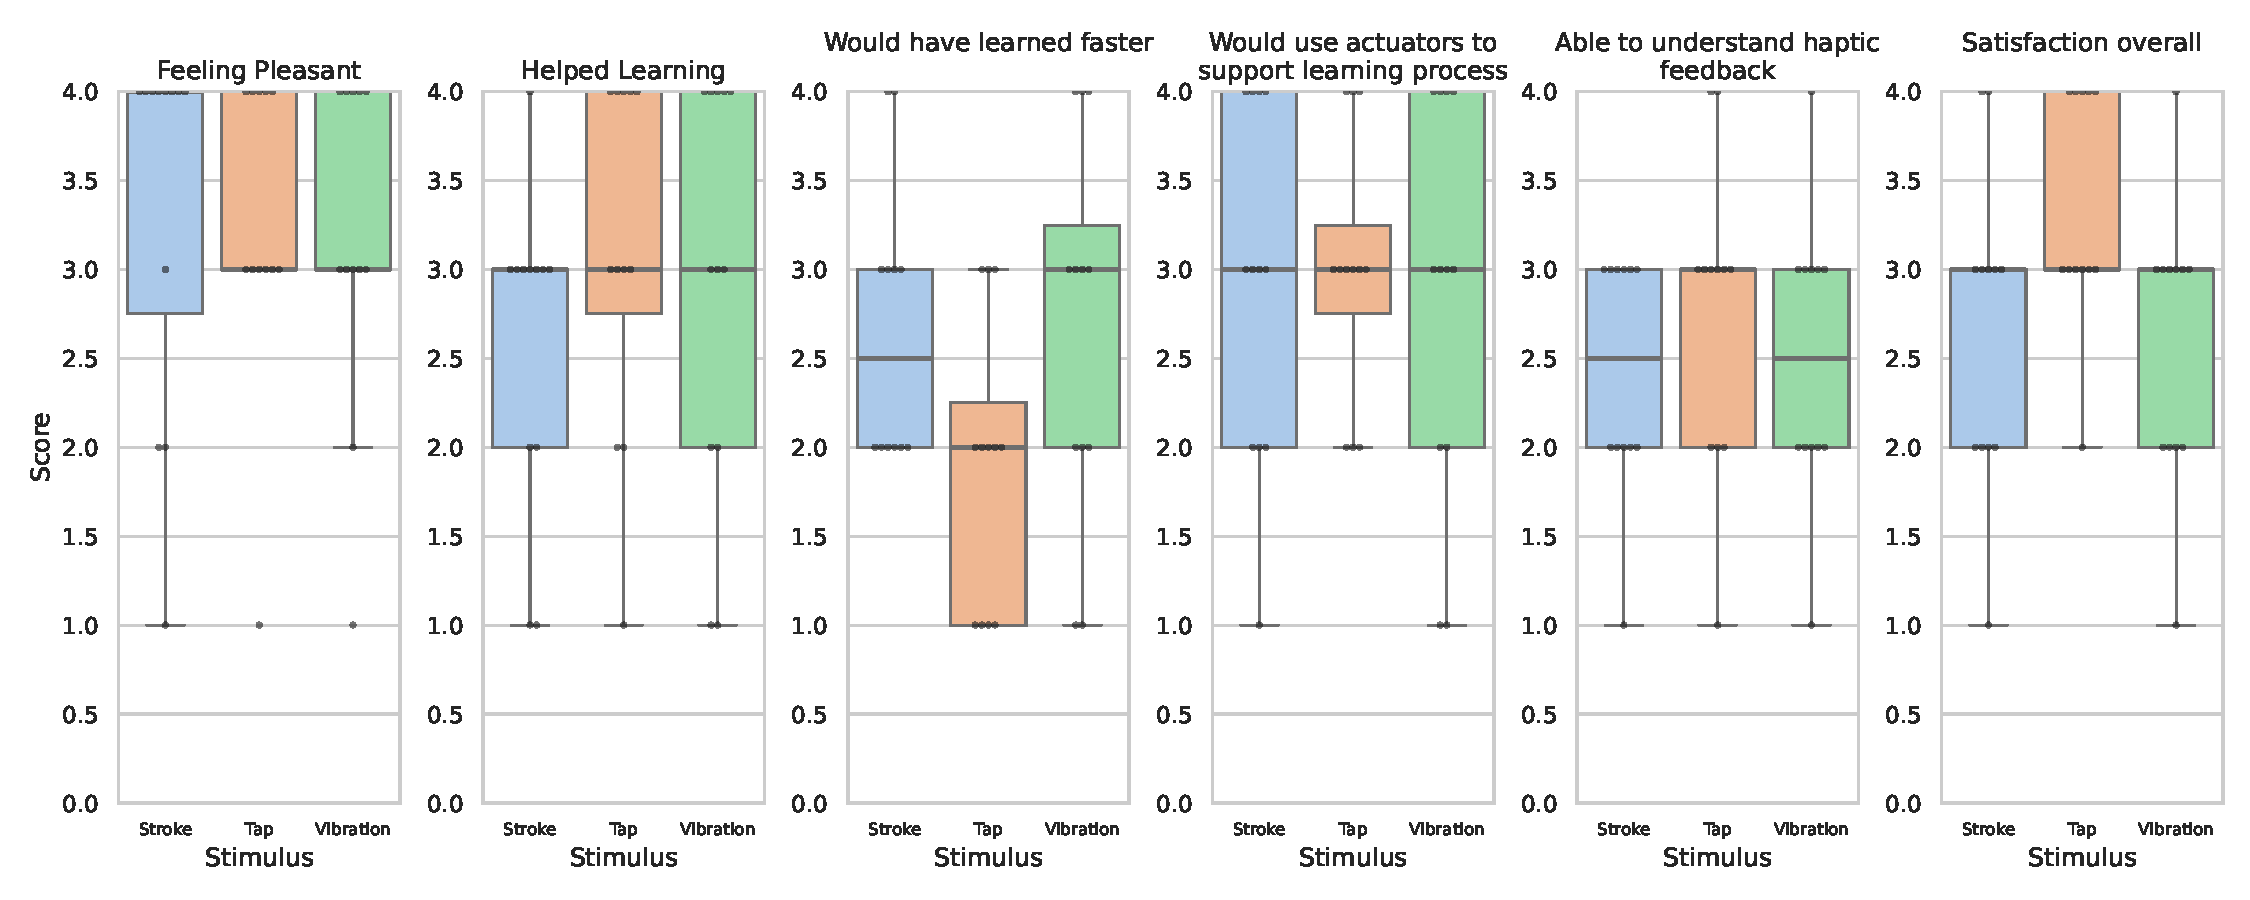
\includegraphics[width=\linewidth]{src/pictures/Study1Data_questionnaire/questions_special_study1.pdf}
    \caption{Self-assessment Results of the different Stimuli grouped by the self-assessment categories.\\4 is the best score and 0 the worst score.\\Each dot represents one participant.}
    \label{fig:questions_individual_firstStudy}
\end{figure}

After the Task Load Index, we surveyed five dimensions to assess how the participants perceived learning and usability with the different actuators, comparing the stimuli across six different dimensions, as shown in \autoref{fig:questions_individual_firstStudy}.

As shown in the figure, there are larger differences in the dimensions \enquote{Helped learning}, \enquote{Would have learned faster}, \enquote{Would use actuators to support the learning process}, and \enquote{Satisfaction overall}.

For the \enquote{Feeling pleasant} dimension, the median values differ by 4 for stroking, and 3 for tapping and vibration. However, the Q1-Q3 quantile ranges are similar, with ranges of 3 to 4 for tapping and vibration, and 2.75 to 4 for stroking. Although the median for stroking is better, there are more outliers for stroking compared to the other two stimuli.

In the \enquote{Helped learning} dimension, the medians are identical for all stimuli, each with a value of 3. However, the quantile ranges differ slightly, with a Q1-Q3 range of 2 to 3 for stroking, 2.75 to 4 for tapping, and 2 to 4 for vibration.

For the \enquote{Would have learned faster} dimension, the medians differ: 2.5 for stroking, 3 for vibration, and 2.0 for tapping, as shown in orange.

In the \enquote{Would use actuators to support the learning process} dimension, the medians are the same for all three stimuli. However, the variance differs considerably, with Q1-Q3 intervals of 2 to 4 for stroking and vibration, while the Q1-Q3 interval for tapping is 2.75 to 3.25.

For \enquote{Satisfaction overall}, the Q1-Q3 intervals are identical for stroking and vibration, ranging from 2 to 3, and from 3 to 4 for tapping. The medians, however, are the same (3.0) for all three stimuli in this dimension.

In the \enquote{Able to understand haptic feedback} dimension, there is no difference in the Q1-Q3 quantile range. However, the medians differ, with 2.5 for stroking and vibration, compared to 3.0 for tapping.


To assess statistical differences, we conducted non-parametric Kruskal-Wallis tests, the results of which are presented in \autoref{table:individualQuestions_significance_firstStudy}.
As shown in the table, no statistically significant differences were found between the stimuli for the dimensions, as the p-values for each Kruskal-Wallis test exceed the threshold value of $\alpha=0.05$.

However, the dimensions closest to the threshold are \enquote{Satisfaction overall} (p-value = 0.0504) and \enquote{Would have learned faster} (p-value = 0.0882). Given their relatively low p-values and \(\eta^2\) effect sizes of 0.1707 and 0.1387 for \enquote{Satisfaction overall} and \enquote{Would have learned faster}, respectively, which are considered large, these dimensions are regarded as \enquote{approaching significance}.


\begin{table}[ht]
\resizebox{\columnwidth}{!}{
\centering
\begin{tabular}{|l|l|l|l|l|}
\hline
\textbf{Question}                              & \textbf{H-statistic}& \textbf{p-value}       & \textbf{Significance}           &\textbf{Effect Size}\\ \hline
\textbf{Feeling Pleasant}                      & 0.706& 0.7026                 & Not Significant                 &0.0202\\ \hline
\textbf{Helped Learning}                       & 1.942& 0.3787                 & Not Significant                 &0.0555\\ \hline
\textbf{Would have learned faster}             & 4.855& 0.0882                 & Not Significant                 &0.1387\\ \hline
\textbf{Would use actuators to support learning process} & 0.038& 0.9812                 & Not Significant                 &0.0011\\ \hline
\textbf{Able to understand haptic feedback}    & 1.241& 0.5377                 & Not Significant                 &0.0355\\ \hline
\textbf{Satisfaction overall}                  & 5.975& 0.0504                 & Not Significant                 &0.1707\\ \hline
\end{tabular}}
\caption{Results of the Kruskal-Wallis significance tests for the different self-assessment dimensions with a $\eta^2$ Effect Size.}
\label{table:individualQuestions_significance_firstStudy}
\end{table}





\begin{figure}
    \centering
    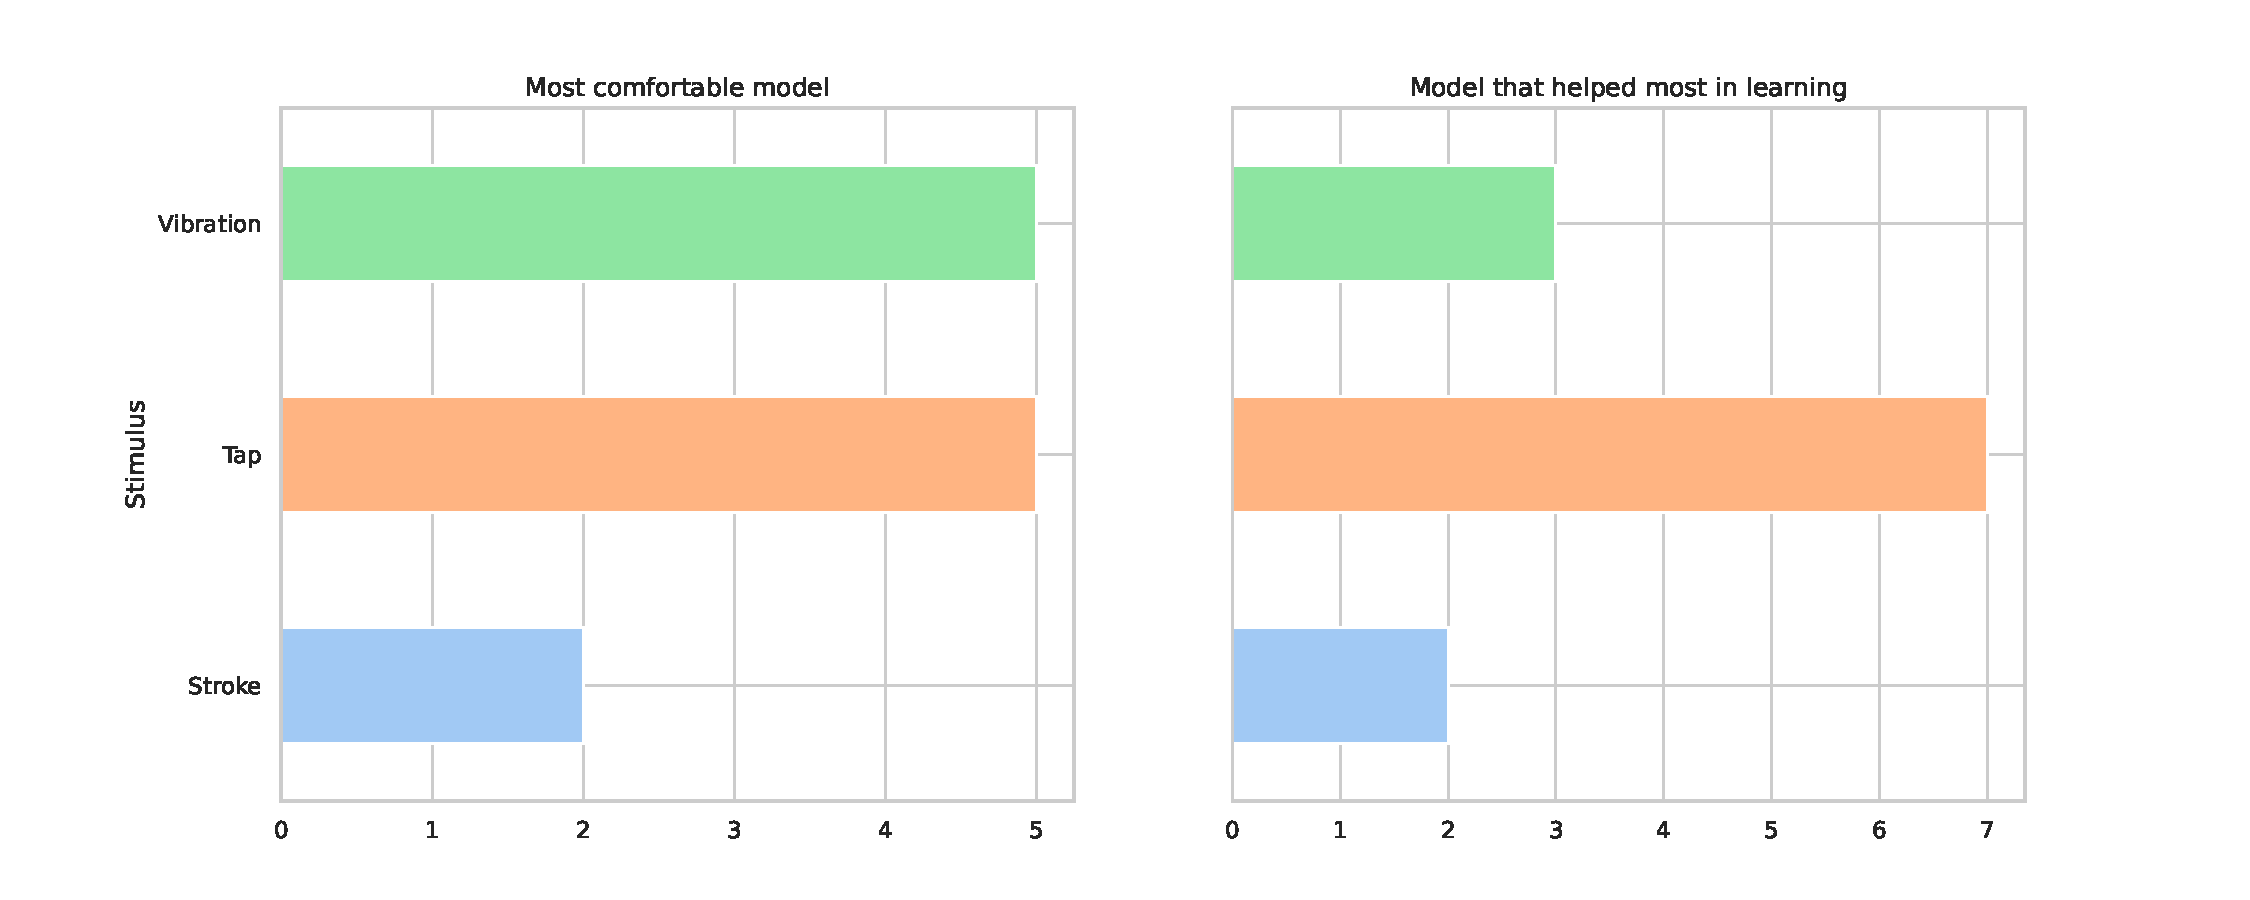
\includegraphics[width=\linewidth]{src/pictures/Study1Data_questionnaire/questions_compare_study1.pdf}
    \caption{Results of the direct comparison between the different stimuli.}
    \label{fig:questionsCompare-firstStudy}
\end{figure}

After completing all the learning sessions for the different stimuli, the participants directly compared the stimuli based on the two dimensions presented in \autoref{fig:questionsCompare-firstStudy}, with the questions \enquote{Which actuator is the most comfortable} on the left and \enquote{Which actuator helped most in learning} on the right. 
$41.67\%$ of the participants found the tapping actuator to be the most comfortable, followed by the vibration actuator, as shown in the left figure, while approximately $16.67\%$ preferred the stroking actuator. This indicates that, according to the participants' judgments, the vibration and tapping actuators were considered superior to the stroking actuators in terms of comfort.

In the \enquote{Which actuator helped most in learning} category, the participants selected the tapping actuator as the most helpful, with $58.33\%$ of participants voting for it, followed by the vibration actuator with $25\%$, and the stroking actuator with $16.67\%$. The stroking actuator was generally perceived as the least effective compared to the other two.

To test for significant statistical differences, we conducted two tests: first, the \gls{csgf}, and, as the sample sizes were relatively small and the expected values might be less than $5$, we performed an additional \gls{emgf}, as suggested by McDonald et al. \cite{mcdonald2014handbook}, because it is likely more accurate. 
The results of these tests are presented in \autoref{table:statistical_tests_comparrisson_firstStudy}. 
As shown, the p-values for the first question, \enquote{Most comfortable model}, are $0.4724$ for the \gls{csgf} and $0.4568$ for the \gls{emgf}, both of which exceed the threshold value of $0.05$. 
The same holds for the question \enquote{Model that helped most in learning}, with p-values of $0.1738$ for the \gls{csgf} and $0.278$ for the \gls{emgf}, indicating that there is no statistically significant difference between the stimuli for those questions.


\begin{table}[ht]
\centering
\resizebox{\columnwidth}{!}{
\begin{tabular}{|l|l|l|l|l|}
\hline
\textbf{Question} & \textbf{Test} & \textbf{Test- Statistic}& \textbf{p-value}  &\textbf{Significance}          \\ \hline
Model most comfortable & \gls{csgf}& 1.5 & 0.4724  &Not Significant                \\
 & \gls{emgf}& 3.464*& 0.4568 &Not Significant                \\\hline
Model that helped most in learning & \gls{csgf}& 3.5 & 0.1738 &Not Significant                \\
 & \gls{emgf}& 4.206*& 0.278 &Not Significant                \\\hline
\end{tabular}}
\caption{Statistical Test Results for the direct comparison between the stimuli.\\\text{*} indicates results obtained via Negative Log-Likelihood under $H_0$.}
\label{table:statistical_tests_comparrisson_firstStudy}
\end{table}

\begin{figure}
    \centering
    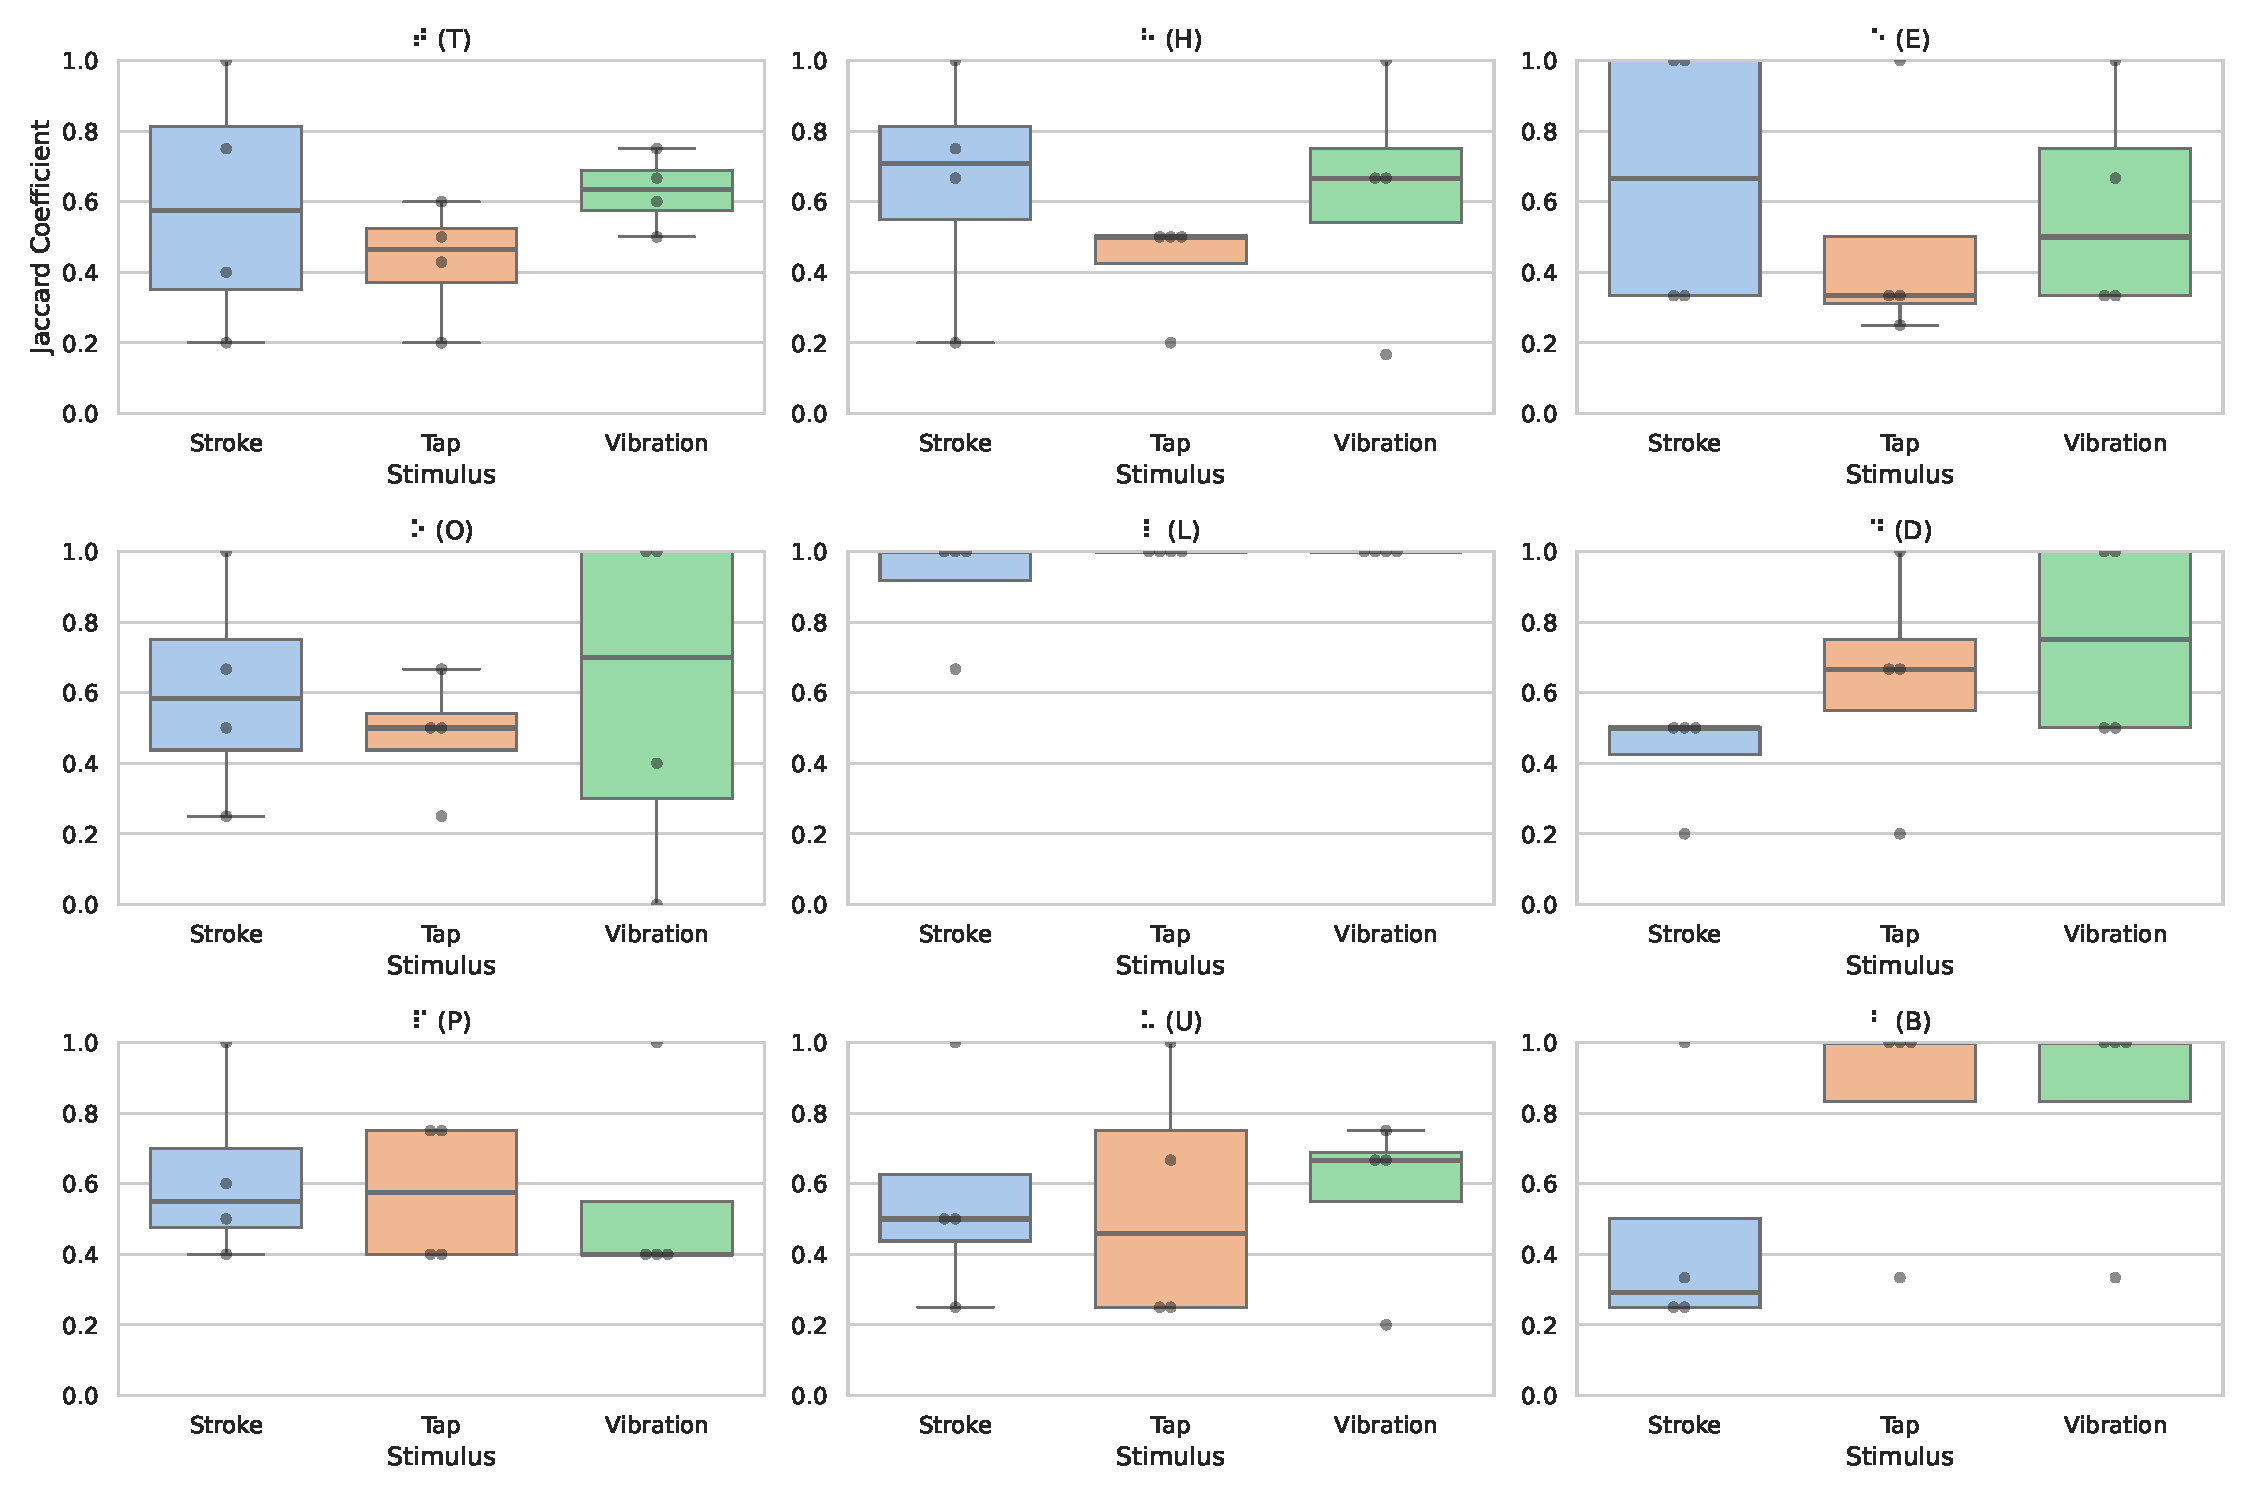
\includegraphics[width=\linewidth]{src/pictures/Study1Data_Experiment/study1_learning_results.pdf}
    \caption{Jaccard coefficient results grouped by the Braille character during learning  for the different stimuli.\\Each dot represents one participant.}
    \label{fig:learning_results_firstStudy}
\end{figure}

After passively learning a character using a specific stimulus, a test was conducted to assess the performance of the characters immediately following the learning session. 
The test results are shown in \autoref{fig:learning_results_firstStudy}, where the stimuli are plotted with their respective Jaccard indices, grouped by the specific characters learned in the session.

The most significant difference is observed for the character \braille{b}(B), where the median for stroking is 0.3, while the medians for tapping and vibration are 1. The quantile ranges for tapping and vibration are 0.82 to 1, while the quantile range for stroking is 0.25 to 0.5.

A similar trend is observed for the character \braille{l}(L), where both tapping and vibration perform perfectly while stroking has an outlier at 0.675. However, all medians are the same at 1.

For the character \braille{h}(H), a larger difference is evident between tapping and the other two stimuli. While tapping has a median of 0.5, the medians for the other two stimuli are approximately 0.7. All three stimuli had a poor outlier, with a score of 0.2.

Another notable difference in medians appears for the character \braille{d}(D), where the median for stroking is 0.5, compared to medians of 0.675 for tapping and 0.75 for vibration. Additionally, the quantile ranges differ: vibration has the largest range, from 0.5 to 1, due to two participants scoring 0.5 and 1, respectively. In contrast, only one participant achieved a perfect score for tapping, and both tapping and stroking have worse participant scores of 0.2.

A further difference can be observed for the character \braille{t}(T), where the median for stroking is approximately 0.6, 0.65 for vibration, and 0.475 for tapping.

To test for significance, we used the Kruskal-Wallis tests. The results, however, did not show any significant differences, as depicted in \autoref{table:learning_significance_results_firstStudy_nonParam_learning}. 
As shown in the \enquote{p-value} column, all p-values for the tests exceed the threshold value of $\alpha = 0.05$, indicating no statistically significant difference between the Jaccard index results of the stimuli for any of the characters.


\begin{table}[ht]
\resizebox{\columnwidth}{!}{
\centering
\begin{tabular}{|l|l|l|l|l|}
\hline
\textbf{Question} & \textbf{Test Statistic} & \textbf{p-value}  &\textbf{Significance}           &\textbf{Effect Size}\\ \hline
\braille{t}(\textbf{T})& 1.9406 & 0.3790  &Not Significant &0.1764\\ \hline
\braille{h}(\textbf{H})& 2.2817& 0.3195&Not Significant &0.2074\\ \hline
\braille{e}(\textbf{E})& 1.1068 & 0.5750  &Not Significant &0.1006\\ \hline
\braille{o}(\textbf{O})& 0.2790& 0.8698&Not Significant &0.0254\\ \hline
\braille{l}(\textbf{L})& 2.0000 & 0.3679  &Not Significant &0.1818\\ \hline
\braille{d}(\textbf{D})& 2.9298& 0.2311&Not Significant &0.2663\\ \hline
\braille{p}(\textbf{P})& 0.7068 & 0.7023  &Not Significant &0.0643\\ \hline
\braille{u}(\textbf{U})& 0.0299& 0.9852&Not Significant &0.0027\\ \hline
\braille{b}(\textbf{B})& 3.6667 & 0.1599  &Not Significant &0.3333\\ \hline
\end{tabular}}
\caption{Results of Kruskal-Wallis significance tests for the different Braille characters during learning with a $\eta^2$ Effect Size.}
\label{table:learning_significance_results_firstStudy_nonParam_learning}
\end{table}



\begin{figure}
    \centering
    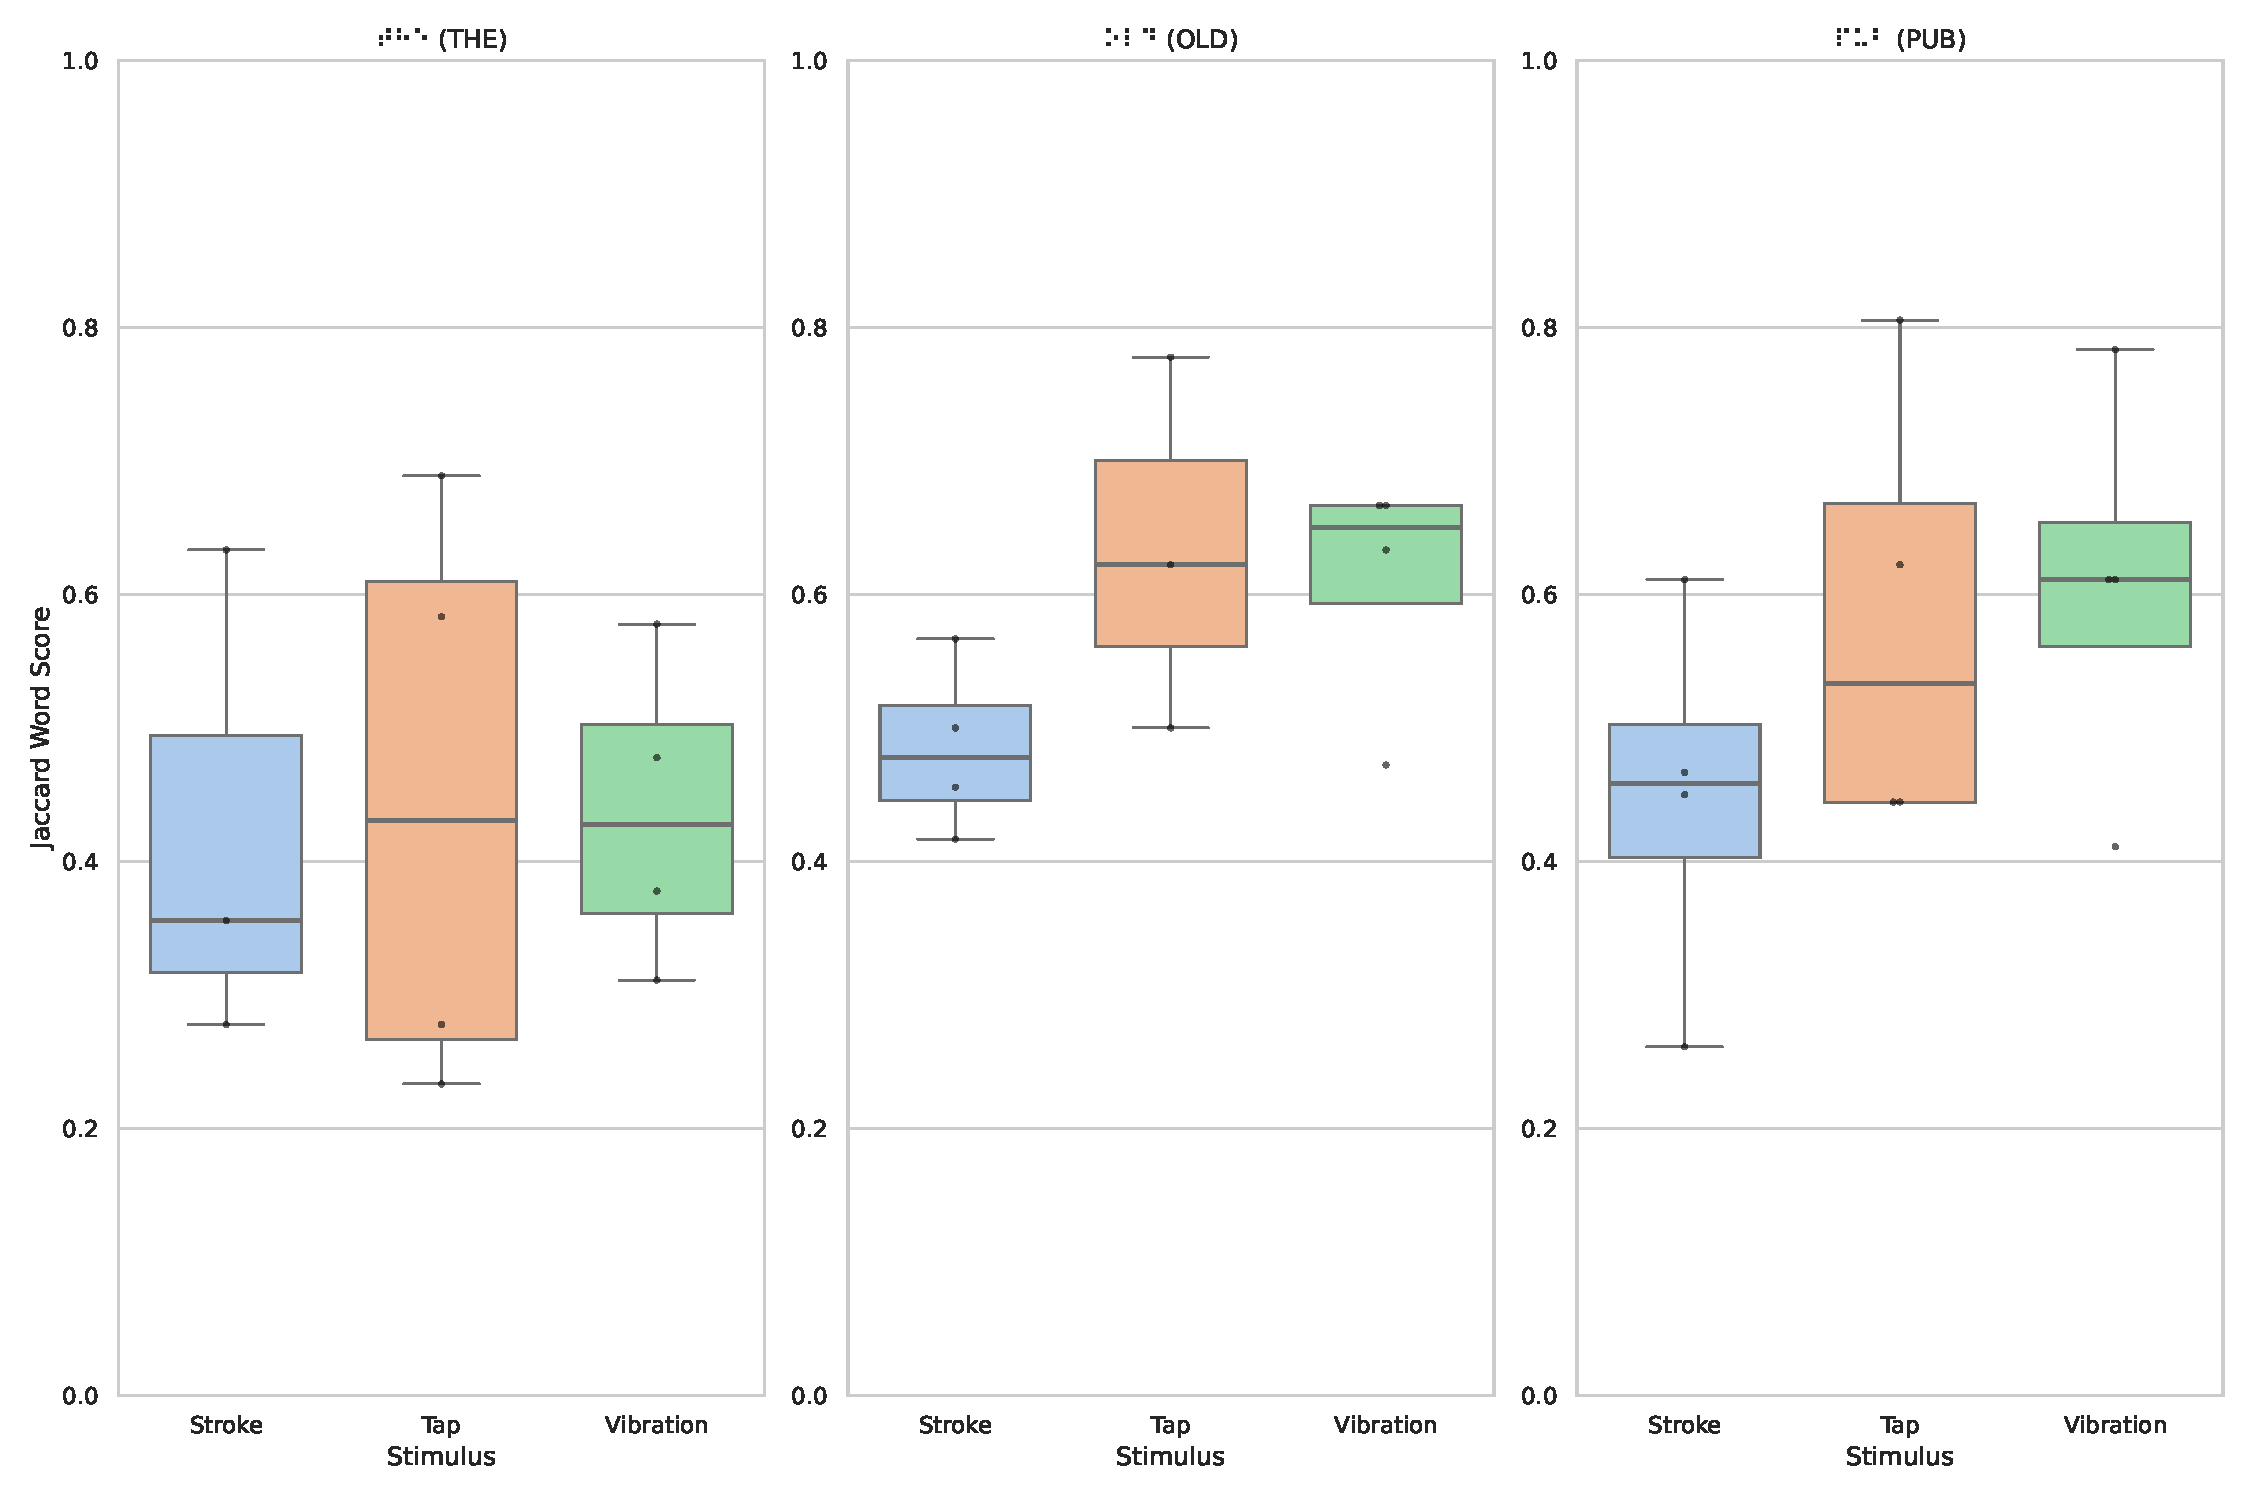
\includegraphics[width=\linewidth]{src/pictures/Study1Data_Experiment/study1_test_results.pdf}
    \caption{Jaccard Word-Test results grouped by the results for the Braille test-words\\
    \enquote{THE}, \enquote{OLD} and \enquote{PUB} for different stimuli.}
    \label{fig:test_results_firstStudy}
\end{figure}



After the passive learning sessions for all characters using a single stimulus, we conducted a word test for the characters learned during the previous passive learning sessions with that stimulus. 
The Jaccard score results, compared across the stimuli for each word, are depicted in \autoref{fig:test_results_firstStudy}. 
As shown, the differences in performance are smaller than those observed for the individual characters. 

For the word \braille{the}(THE), the medians are 0.375 for stroking, 0.425 for tapping, and 0.425 for vibration. The quantile ranges are 0.35-0.5 for stroking, 0.3-0.6 for tapping, and 0.475-0.45 for vibration, respectively.

For the word \braille{old}(OLD), the medians are 0.62 for tapping and 0.625 for vibration, compared to 0.475 for stroking.

For the word \braille{pub}(PUB), the median for stroking (0.45) is somewhat lower than that for tapping (0.56) and vibration (0.61). 

Additionally, it can be observed that the quantile range for tapping is almost twice as large as that of the other two stimuli, with an approximate range of 0.2 compared to 0.1 for both vibration and stroking.

To test for significance, we performed a Kruskal-Wallis test, the results of which are depicted in \autoref{table:significance_results_test_firstStudy}. 
The results showed that all p-values are well above the threshold $\alpha$, with the closest value being 0.1371 for the word \braille{old}(OLD). 
This indicates that there was no statistically significant difference between the Jaccard index results for the different stimuli in relation to the word tests.

\begin{table}[ht]
\resizebox{\columnwidth}{!}{
\centering
\begin{tabular}{|l|l|l|l|l|}
\hline
\textbf{Question} & \textbf{Test Statistic} & \textbf{p-value}  &\textbf{Significance}           &\textbf{Effect Size}\\ \hline
\braille{the}(\textbf{THE})& 0.0361& 0.9821&Not Significant &0.0036\\ \hline
\braille{old}(\textbf{OLD})& 3.9736 & 0.1371  &Not Significant &0.1371\\ \hline
\braille{pub}(\textbf{PUB})& 1.0569& 0.5895&Not Significant &0.0961\\ \hline
\end{tabular}}
\caption{Results of the Kruskal-Wallis significance tests for the wordtests \enquote{THE}, \enquote{OLD}, and \enquote{PUB} with a $\eta^2$ Effect Size.}
\label{table:significance_results_test_firstStudy}
\end{table}



\begin{figure}
    \centering
    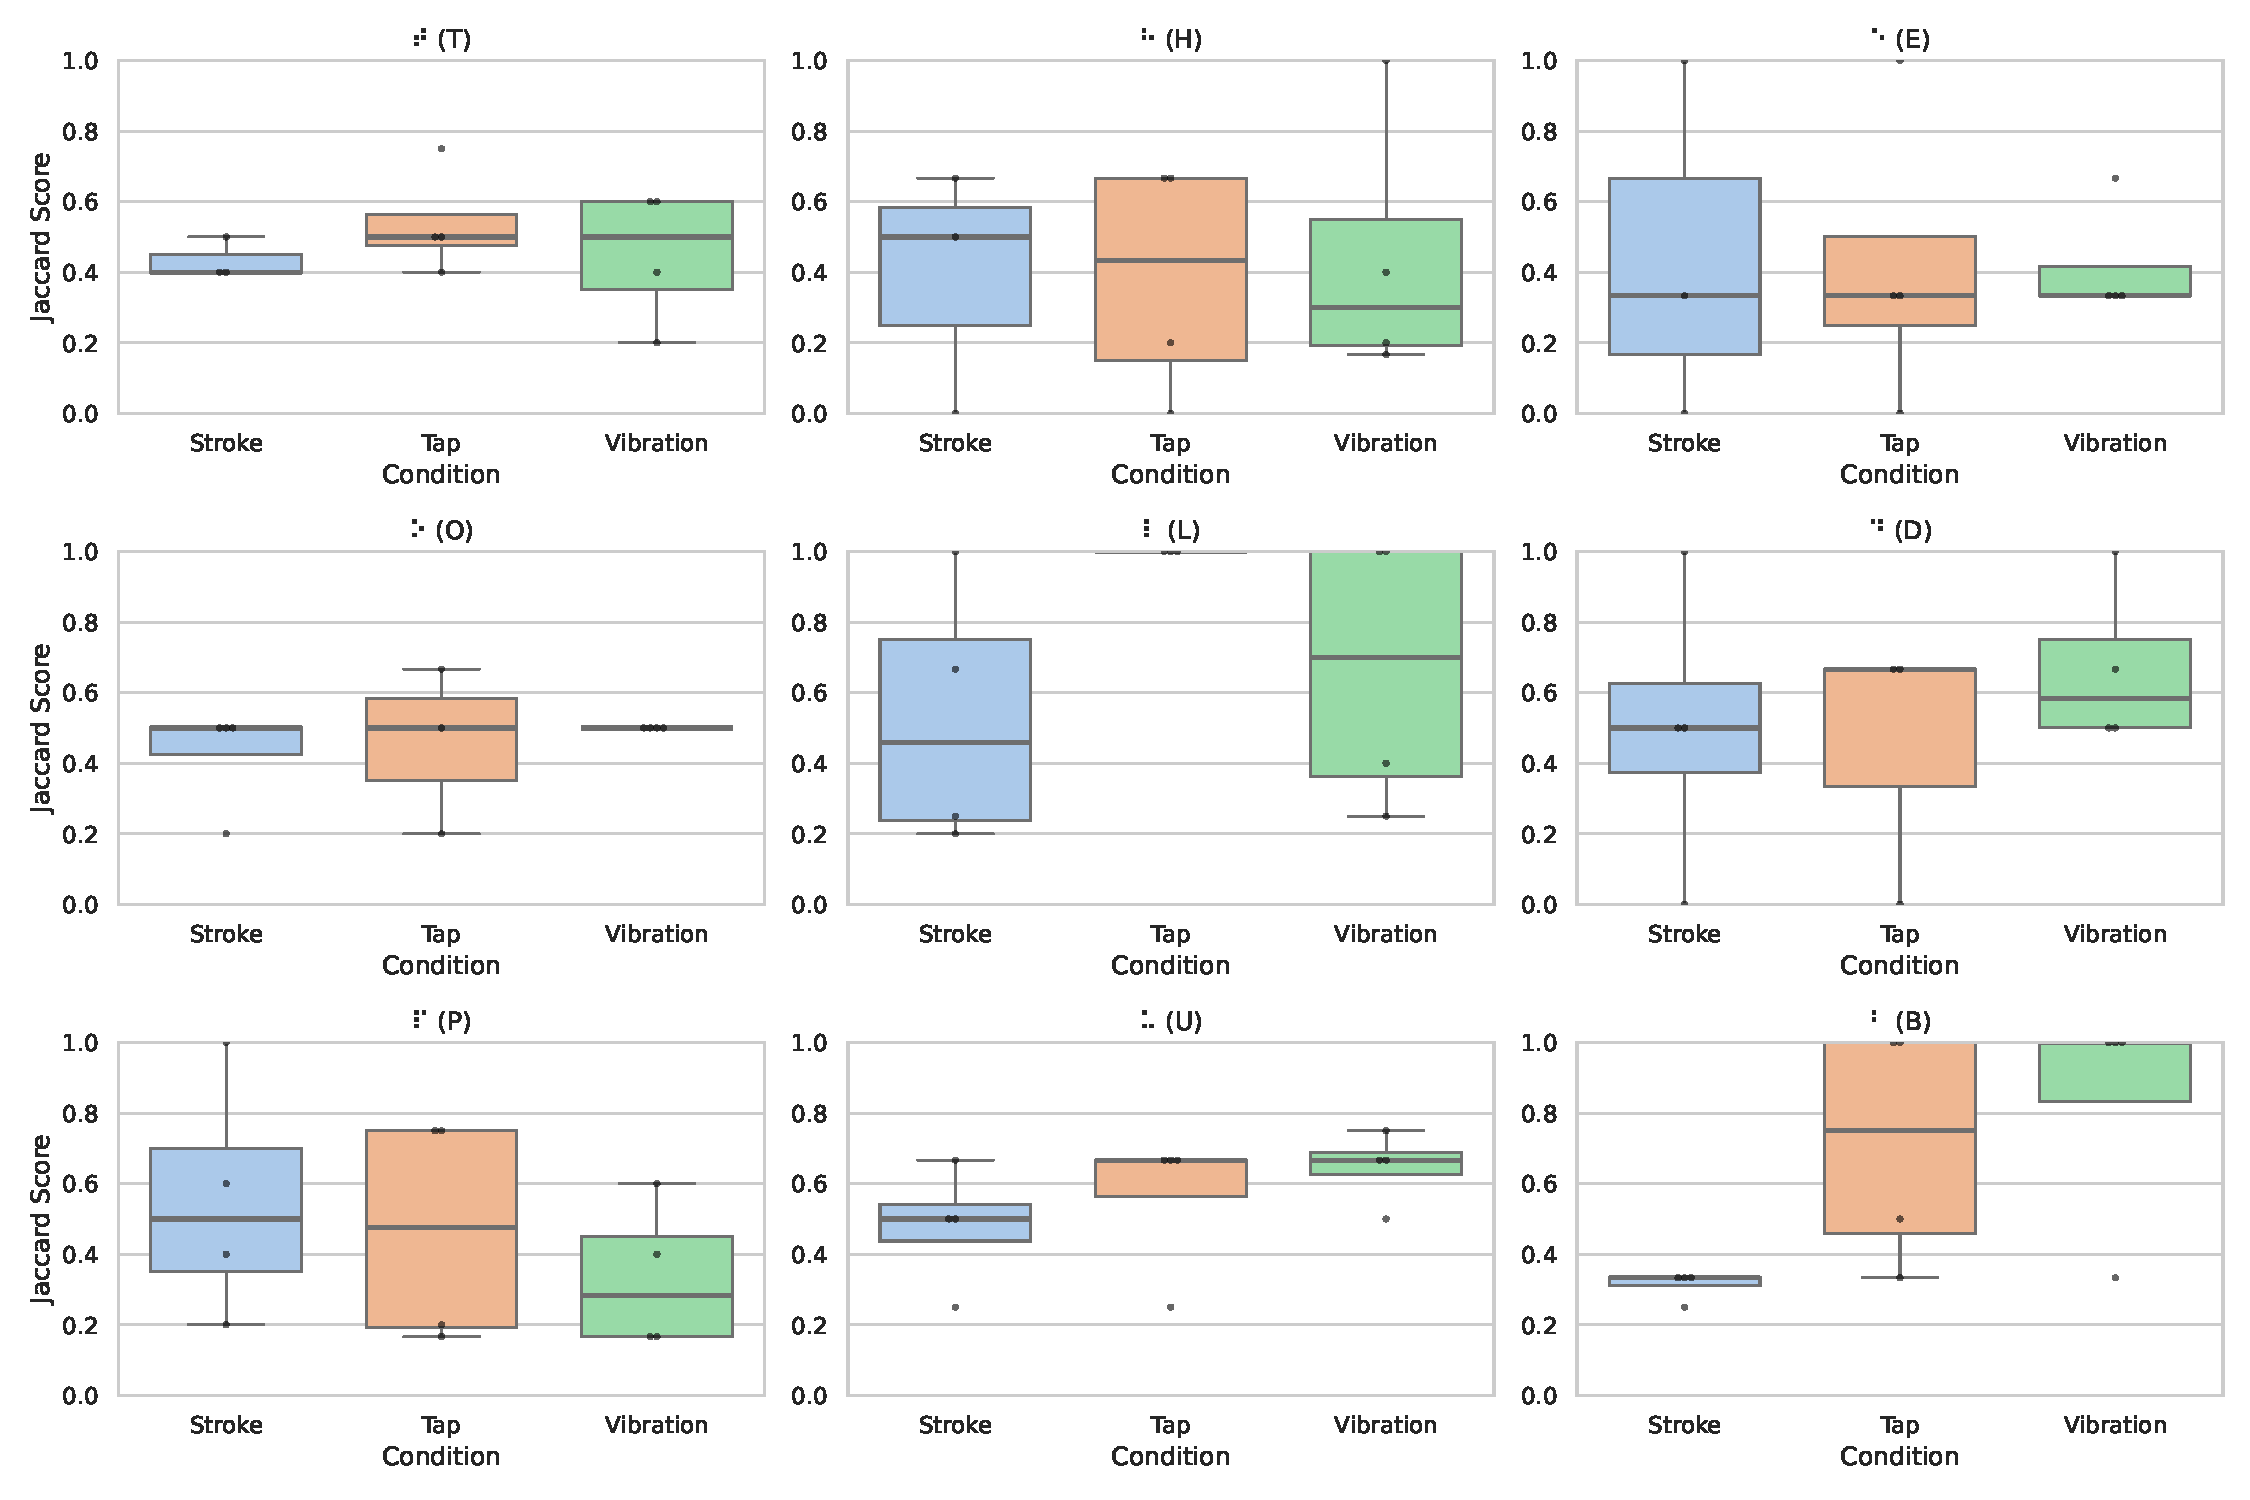
\includegraphics[width=\linewidth]{src/pictures/Study1Data_Experiment/character_jaccard_test_study1.pdf}
    \caption{Jaccard Score comparison for the different Stimuli grouped by the Braille test-word characters.}
    \label{fig:jaccard_test_study1}
\end{figure}


We further investigated the results by breaking them down for each individual character and analyzing them by examining false positives and false negatives in the construction of the Jaccard score. 
We regarded the decision to press a key or not as a classification task. 
Thus, a "missed character" is classified as a false negative, and a "surplus character" is classified as a false positive. 
Using this approach, we calculated precision and recall to derive the Jaccard score. 
These values are plotted in \autoref{fig:jaccard_test_study1}. 

As shown in the plot, the Jaccard score values do not differ significantly across most of the boxplots. 
The largest differences are observed for the character \braille{l}(L), where tapping performed the best with a median of 1 while stroking performed the worst with a median of 0.45 and vibration had a median of 0.7. 
Although perfect scores are observed for all stimuli, stroking had more low data points, with Jaccard scores of 0.2 and 0.25.

The character \braille{b}(B) showed a different pattern, with a median of approximately 0.325 for stroking, 0.75 for tapping, and 1 for vibration. 
None of the stroking participants were able to press the correct keys, whereas 2 participants in the tapping condition and 3 in the vibration condition succeeded in learning the character.

Additional differences were noted for the characters \braille{d}(D) and \braille{p}(P). 
For \braille{p}(P), the median for stroking was higher than the other stimuli, with a median of 0.5 compared to 0.45 for tapping and 0.3 for vibration. 

For \braille{d}(D), stroking was the worst-performing stimulus, with a median of 0.5 compared to 0.6 for tapping and 0.58 for vibration. 
It is important to note that there was only one perfect score for both vibration and stroking, while there were also scores of 0 for both stroking and tapping.

However, when testing for statistical significance using Kruskal-Wallis tests, which are tabulated in \autoref{table:learning_significance_results_firstStudy_nonParam}, no significant differences were found for any stimulus across the characters, with the exception of \braille{b}(B), which approached significance with a p-value of 0.0559 and a large \(\eta^2\) effect size of 0.3906.


\begin{table}[ht]
\resizebox{\columnwidth}{!}{
\centering
\begin{tabular}{|l|l|l|l|l|}
\hline
\textbf{Question} & \textbf{Test Statistic} & \textbf{p-value}  &\textbf{Significance}           &\textbf{Effect Size}\\ \hline
\braille{t}(\textbf{T})& 1.0203& 0.6004&Not Significant &0.1131\\ \hline
\braille{h}(\textbf{H})& 0.0136& 0.9932&Not Significant &0.0017\\ \hline
\braille{e}(\textbf{E})& 0.0979& 0.9522&Not Significant &0.0121\\ \hline
\braille{o}(\textbf{O})& 0.5309& 0.7669&Not Significant &0.0622\\ \hline
\braille{l}(\textbf{L})& 3.3764& 0.1849&Not Significant &0.2968\\ \hline
\braille{d}(\textbf{D})& 0.5290& 0.7676&Not Significant &0.0620\\ \hline
\braille{p}(\textbf{P})& 1.6124& 0.4465&Not Significant &0.1519\\ \hline
\braille{u}(\textbf{U})& 2.5488& 0.2796&Not Significant &0.2207\\ \hline
\braille{b}(\textbf{B})& 5.7683& 0.0559&Not Significant &0.3906\\ \hline
\end{tabular}}
\caption{Results of Kruskal-Wallis significance tests for the different Braille characters during testing with a $\eta^2$ Effect Size.}
\label{table:learning_significance_results_firstStudy_nonParam}
\end{table}





\begin{figure}
    \centering
    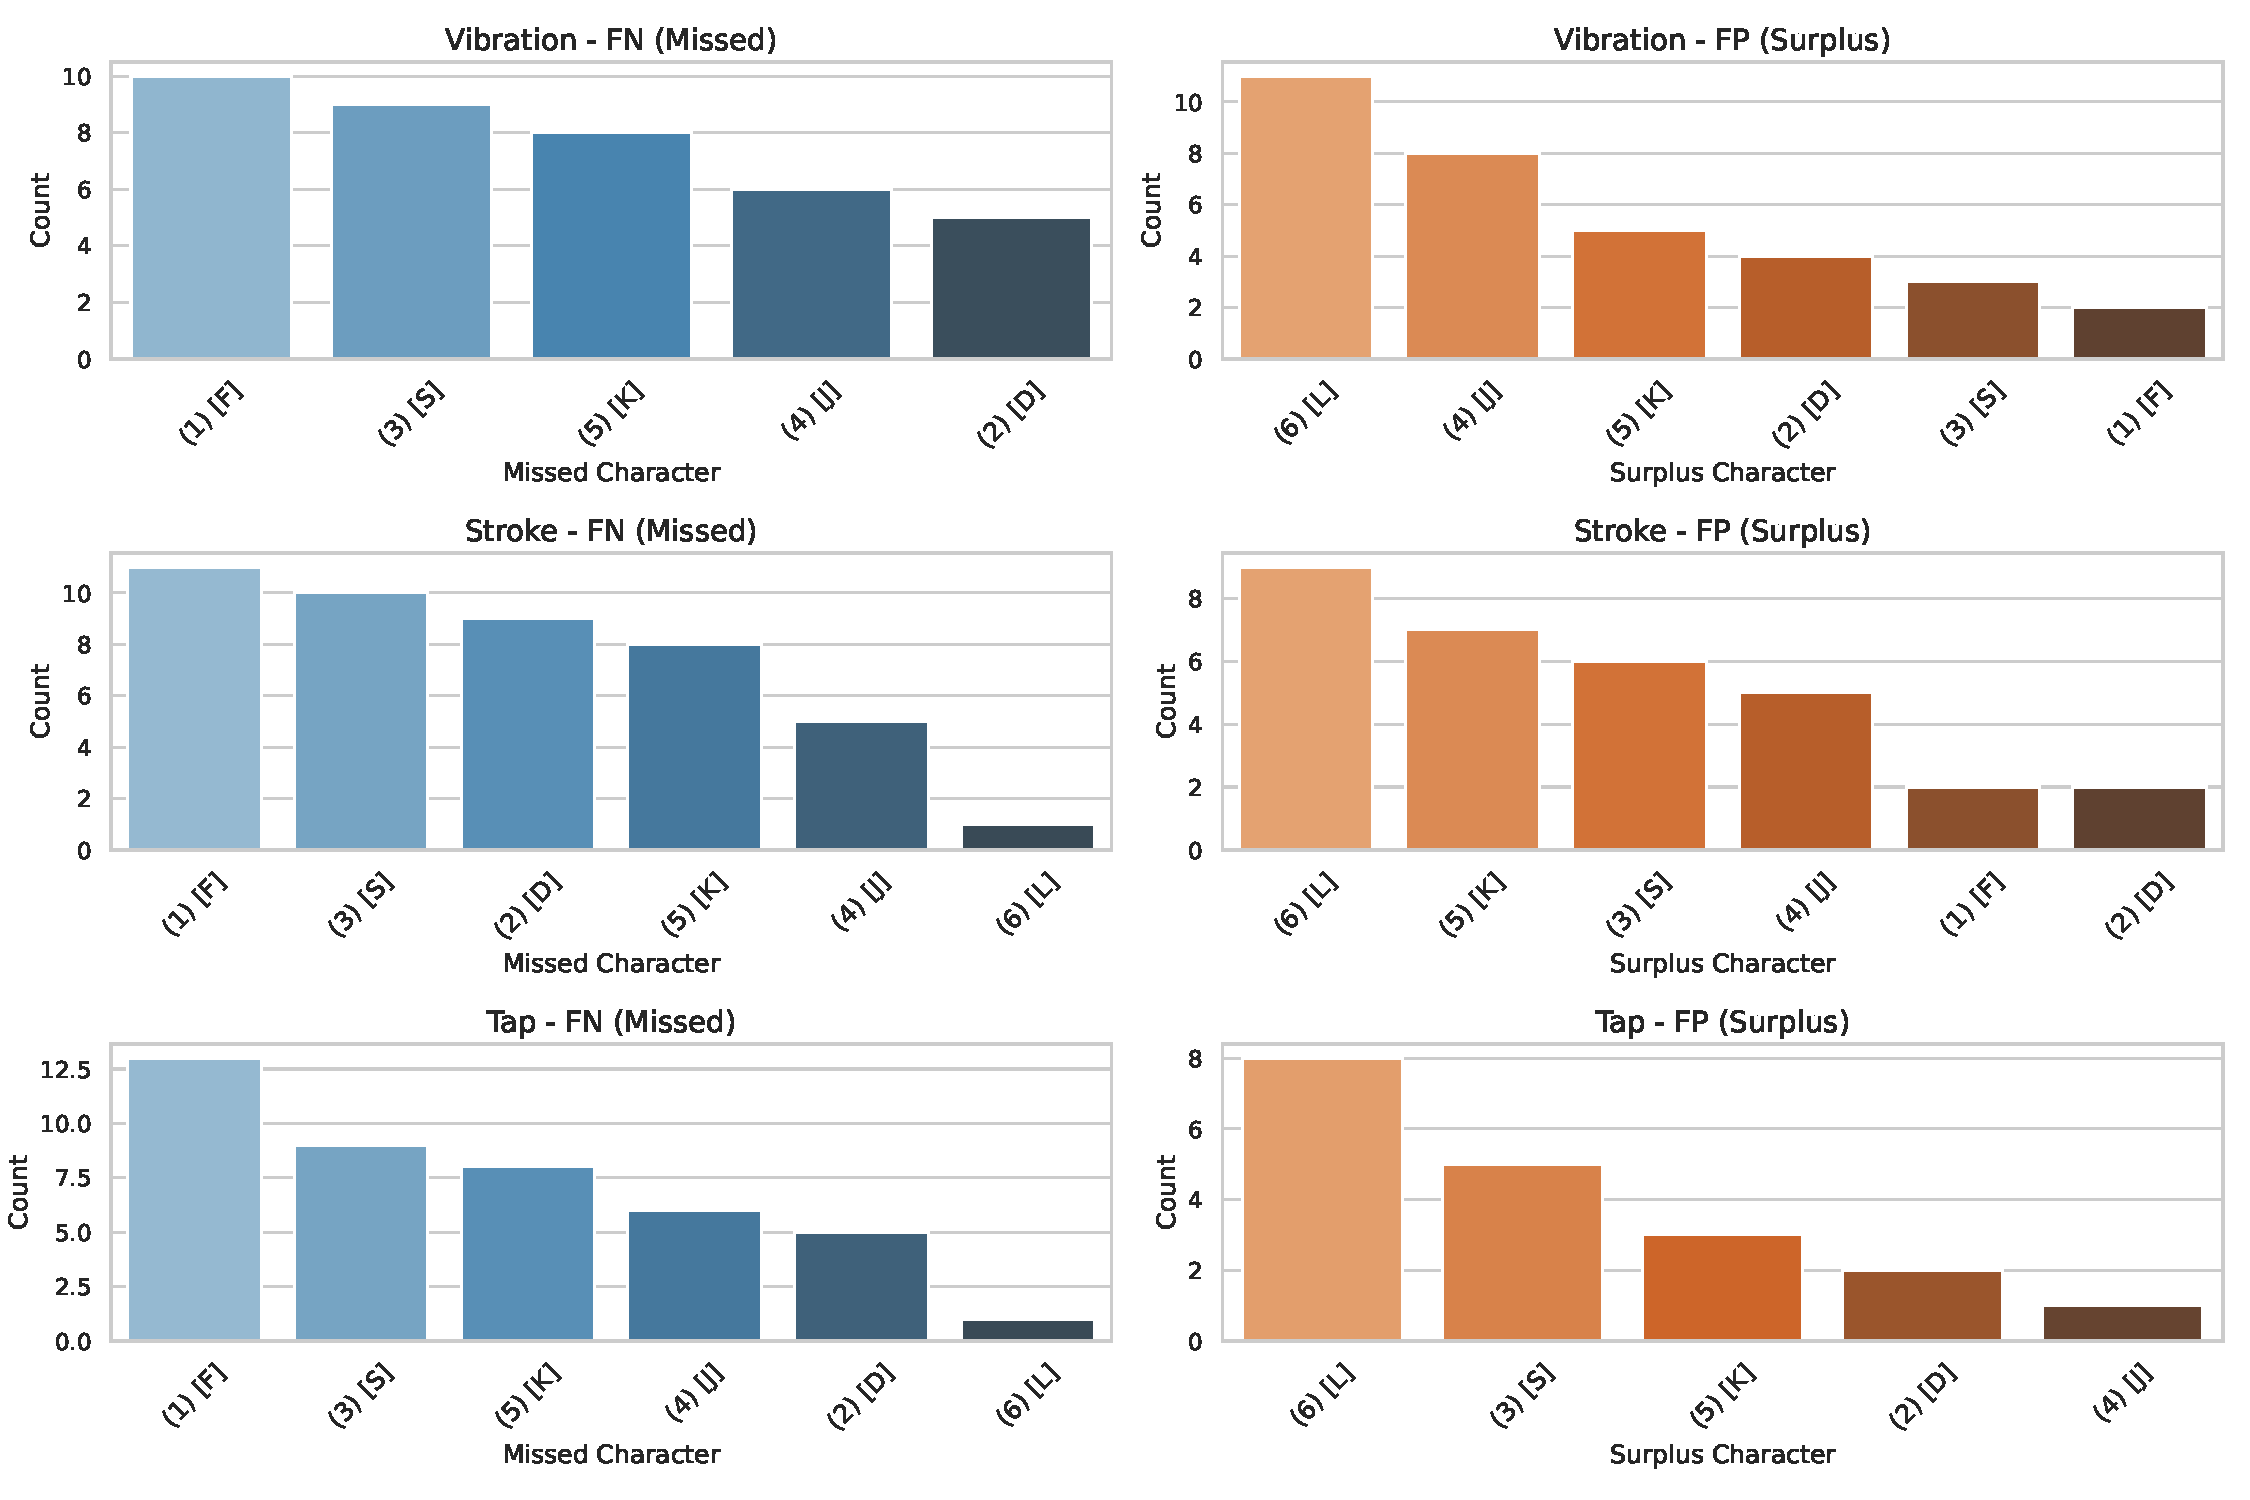
\includegraphics[width=\linewidth]{src/pictures/Study1Data_Experiment/missed_surplus_test_study1.pdf}
    \caption{FN  (Missed) and FP (Surplus) key(s) for each stimuli.}
    \label{fig:missedSurplus_study1}
\end{figure}

To analyse the data that contributed to the Jaccard scores previously presented, we further examined the missed and surplus characters—those that were either missed or incorrectly submitted in addition to the required characters during the test. 
The results for the missed and surplus characters are depicted in \autoref{fig:missedSurplus_study1}, grouped by the stimulus.

As shown for the false negative characters (missed characters), marked in blue on the left side, the first two missed characters are always \textcircled{1} [F] and \textcircled{3} [S], followed by \textcircled{4} [K] for both the vibration and tapping stimuli. 
For the stroking stimulus, \textcircled{2} [D] follows, and then \textcircled{4} [K]. 
The character \textcircled{6} [L] was the least missed, as it does not appear among the missed characters for the vibration stimulus and ranks last for both the stroking and tapping stimuli. 
Next, the character \textcircled{2} [D] appears, which is ranked last for vibration and second-to-last for tapping. 
Following this, \textcircled{4} [J] is the second-to-last missed character for the vibration and stroking stimuli, and ranks third from the bottom for the tapping stimulus.

For the false positives (surplus characters), shown in red on the right, the most frequently added character is \textcircled{6} [L]. 
This indicates that, in most cases, the character \textcircled{6} [L] was added too often. However, the specific differences between the actuators vary. 
The \textcircled{1} [F] character appears last for the vibration stimulus, second-to-last for the stroking stimulus, and was never added as a surplus for the tapping stimulus.


\begin{figure}[h!]
    \centering
    \begin{subfigure}[b]{0.45\textwidth}
        \centering
        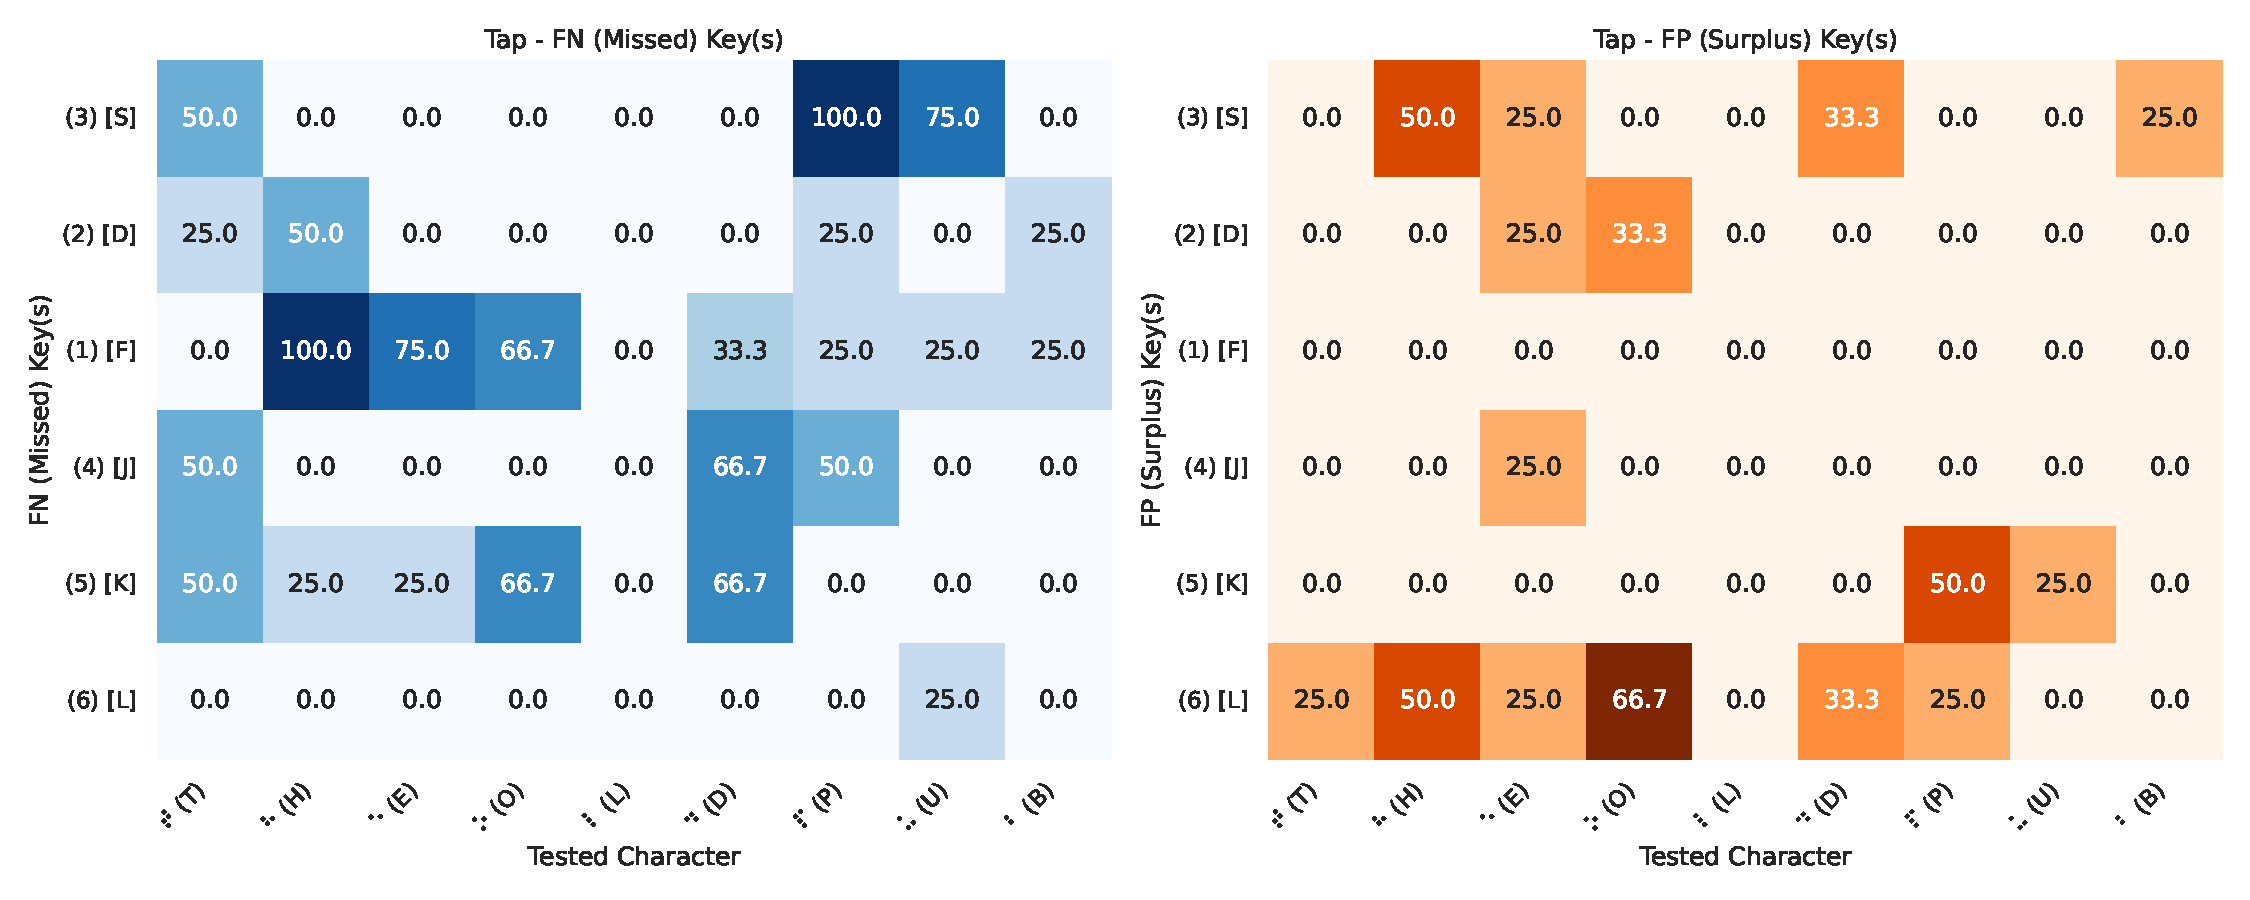
\includegraphics[width=\textwidth]{src/pictures/Study1Data_Experiment/missed_surplus_test_percentages_study1_T.pdf}
        \caption{Tapping Stimulus}
    \end{subfigure}
    \begin{subfigure}[b]{0.45\textwidth}
        \centering
        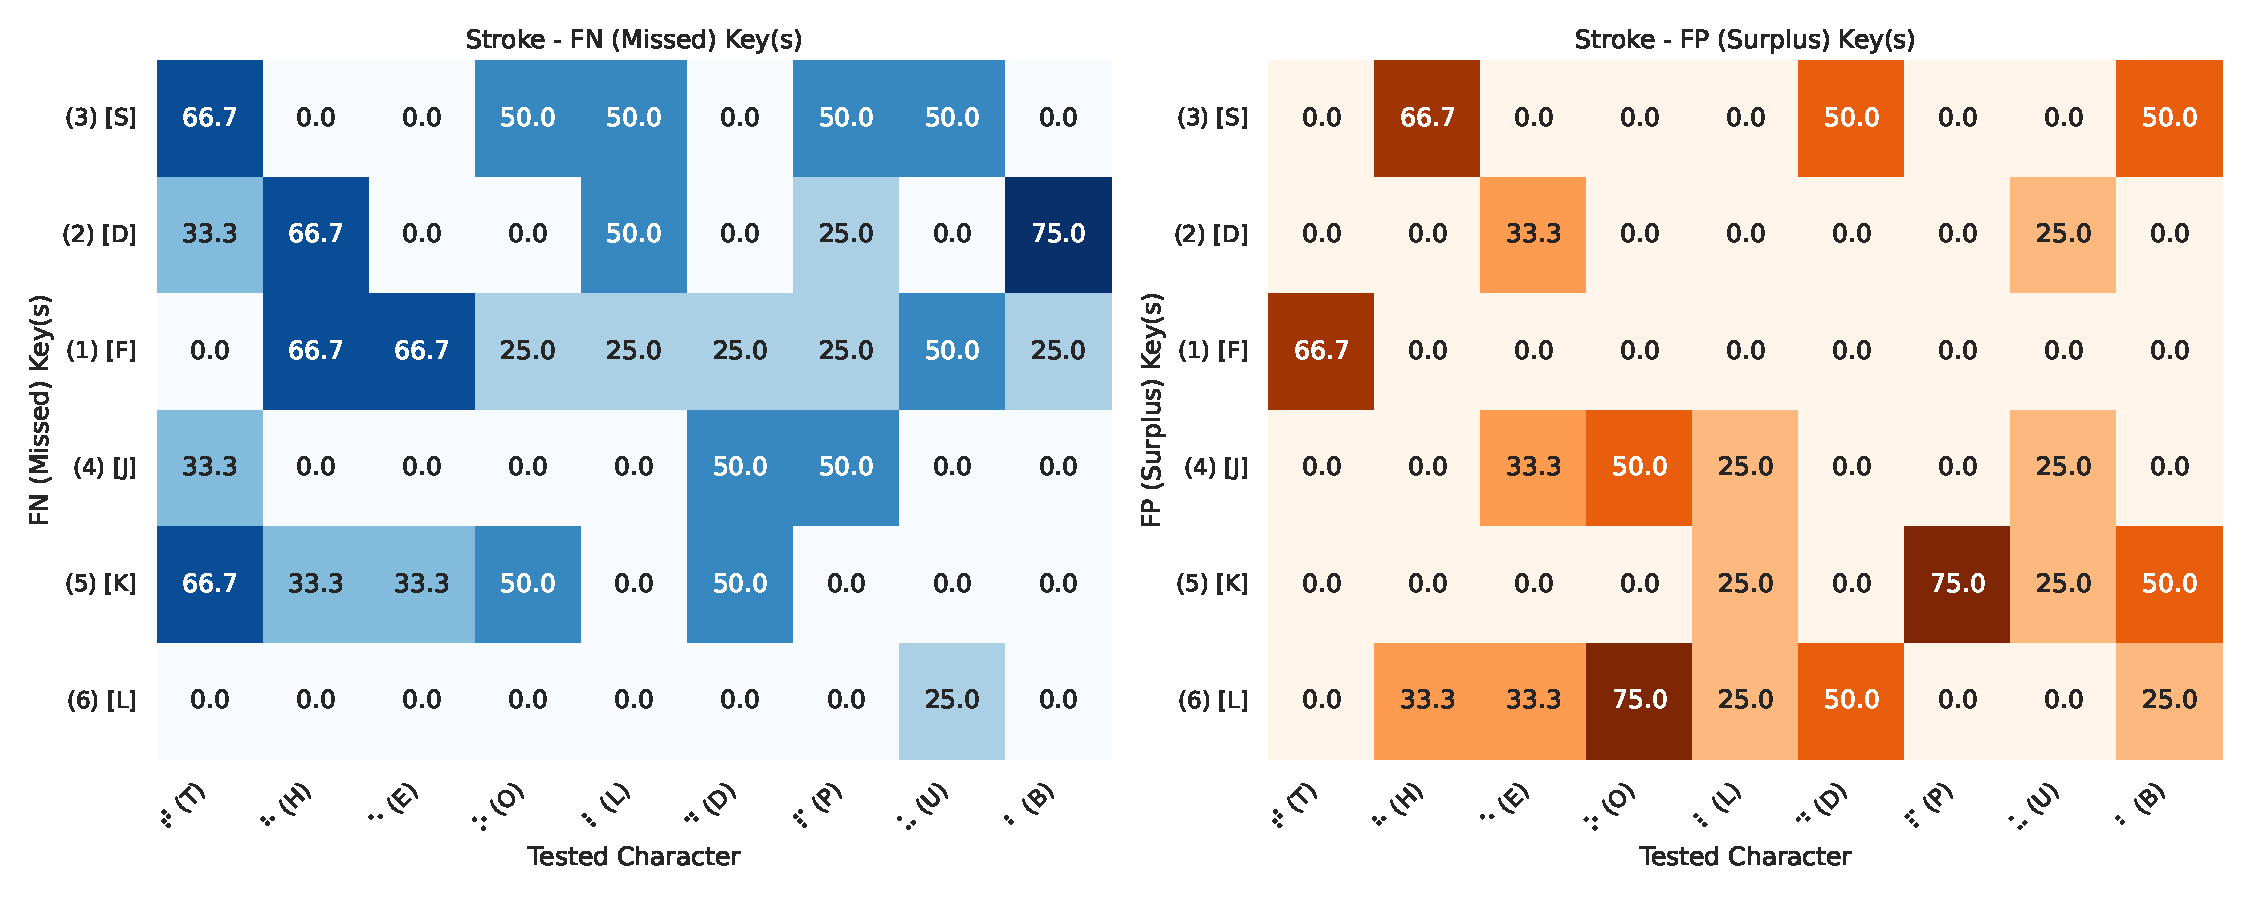
\includegraphics[width=\textwidth]{src/pictures/Study1Data_Experiment/missed_surplus_test_percentages_study1_S.pdf}
        \caption{Stroking Stimulus}
    \end{subfigure}\\
    \begin{subfigure}[b]{0.45\textwidth}
        \centering
        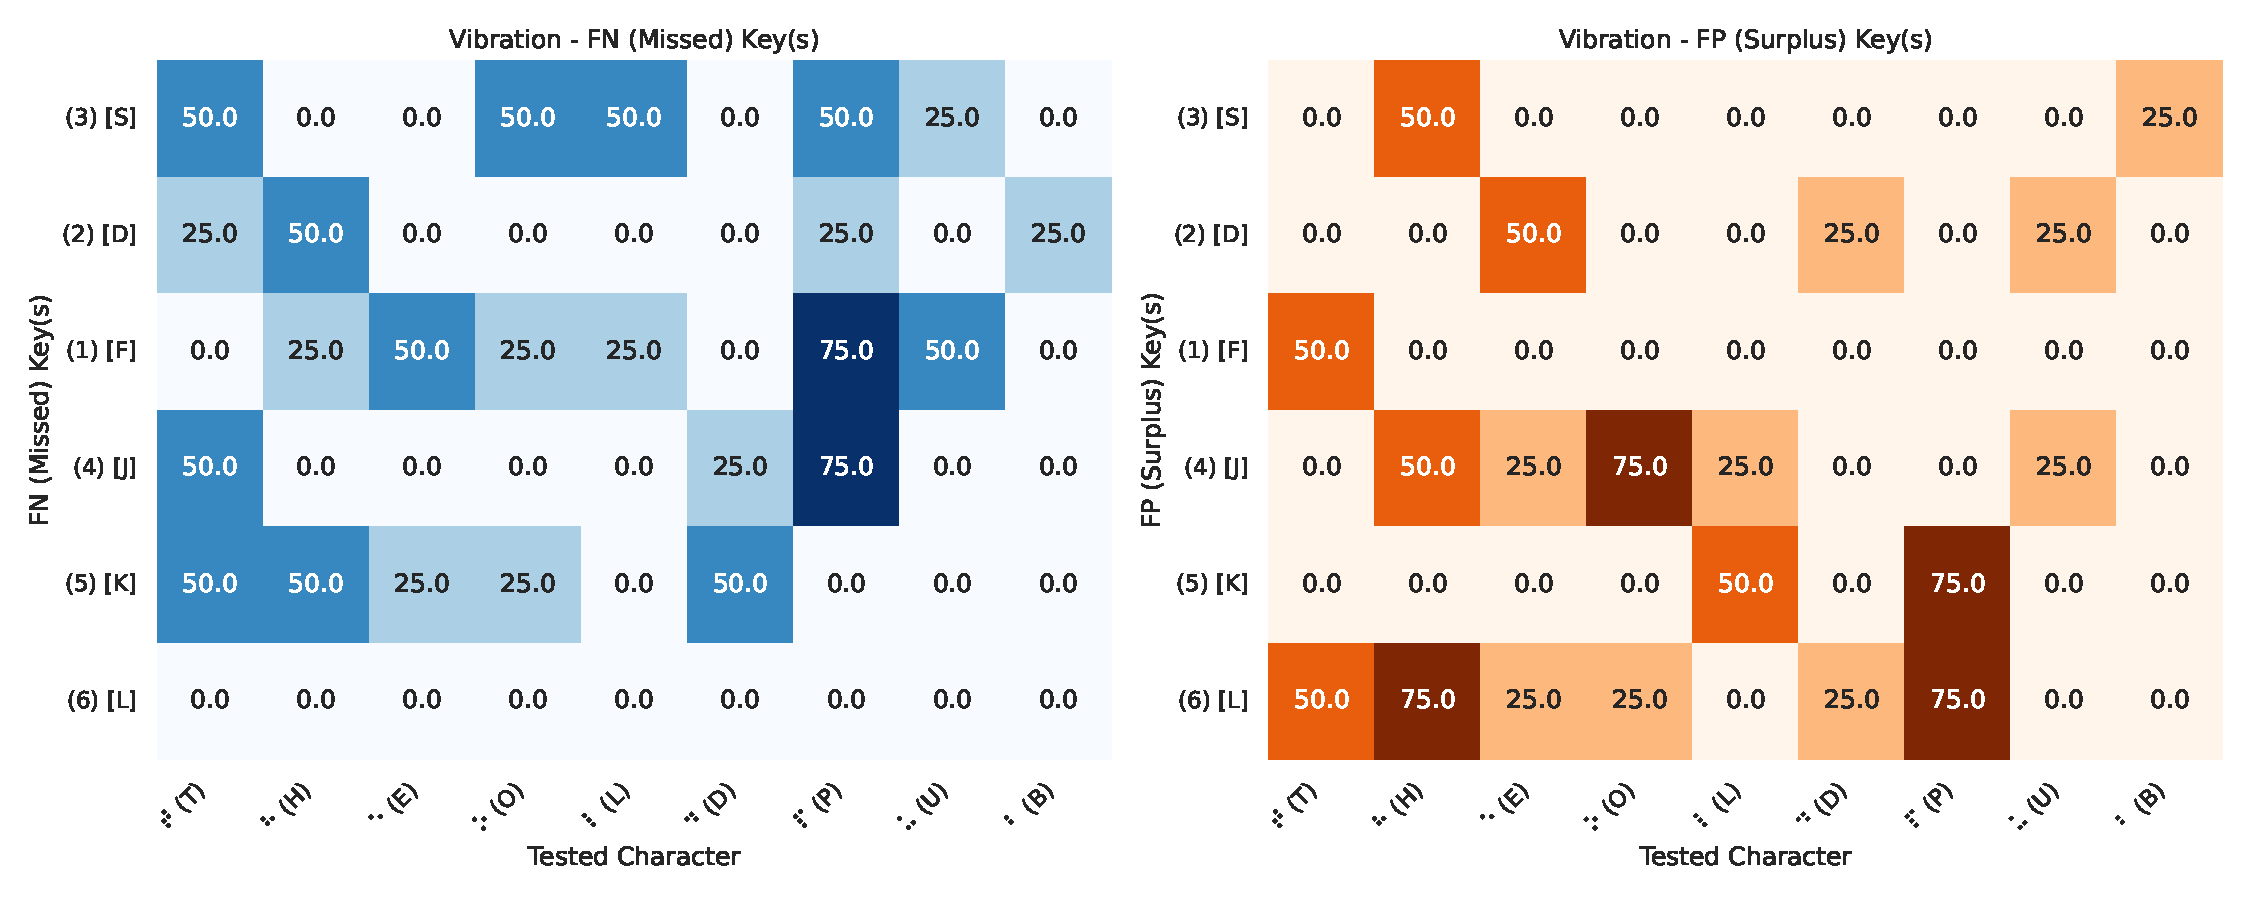
\includegraphics[width=\textwidth]{src/pictures/Study1Data_Experiment/missed_surplus_test_percentages_study1_V.pdf}
        \caption{Vibration Stimulus}
    \end{subfigure}
    \caption{FN (Missed) Character in blue and FP (Surplus) keys in red in percent for each Braille character grouped by stimulus.}
    \label{fig:missed_surplus_percentages_study1}
\end{figure}

After analysing the missed and surplus characters, we now dive deeper into the specific relationships between each tested character and the corresponding surplus or missed character. These details are depicted in \autoref{fig:missed_surplus_percentages_study1}.

The diagram shows each Braille character under the category \enquote{tested character}, with the corresponding pressed keyboard characters on the left. 
The blue sections represent the percentage of missed keys when typing a character, while the red sections indicate surplus pressed keys for each character.

It is important to note that both \autoref{fig:missed_surplus_percentages_study1} and \autoref{fig:missedSurplus_study1} are related. Each column in \autoref{fig:missedSurplus_study1} corresponds to one row of missed or surplus characters in the same stimulus image, with matching colours for the same character. 
Thus, \autoref{fig:missed_surplus_percentages_study1} provides a more detailed, lower-level abstraction of the data shown in \autoref{fig:missedSurplus_study1}.

For the surplus (red) side, significant differences are observed for the Braille characters \braille{b}(B) and \braille{u}(U). For \braille{b}(B), the key \textcircled{3} [S] was consistently pressed incorrectly across all stimuli. However, for the Stroking stimulus, the keys \textcircled{5} [K] and \textcircled{5} [L] were also pressed incorrectly, with percentages of 50\% and 25\%, respectively.

Another notable difference occurs for the Braille character \braille{u}(U), where the key \textcircled{4} [K] was pressed incorrectly for the Tap and Stroking stimuli, and the keys \textcircled{4} [J] and \textcircled{2} [D] were pressed incorrectly for the Stroking and Vibration stimuli.

For the missed characters (FN, in blue), several differences are evident for the Braille characters \braille{l}(L) and \braille{b}(B). There were no missed characters for the Tapping stimulus, but for the Stroking and Vibration stimuli, the keys \textcircled{3} [S] and \textcircled{1} [F] were frequently missed. In the case of Stroking, the key \textcircled{2} [D] was missed in about 50\% of the trials.

A larger difference is seen with the key \textcircled{6} [L], which was never missed for the Vibration stimulus but was missed in about 25\% of cases for both the Stroking and Tapping stimuli.

\begin{figure}
    \centering
    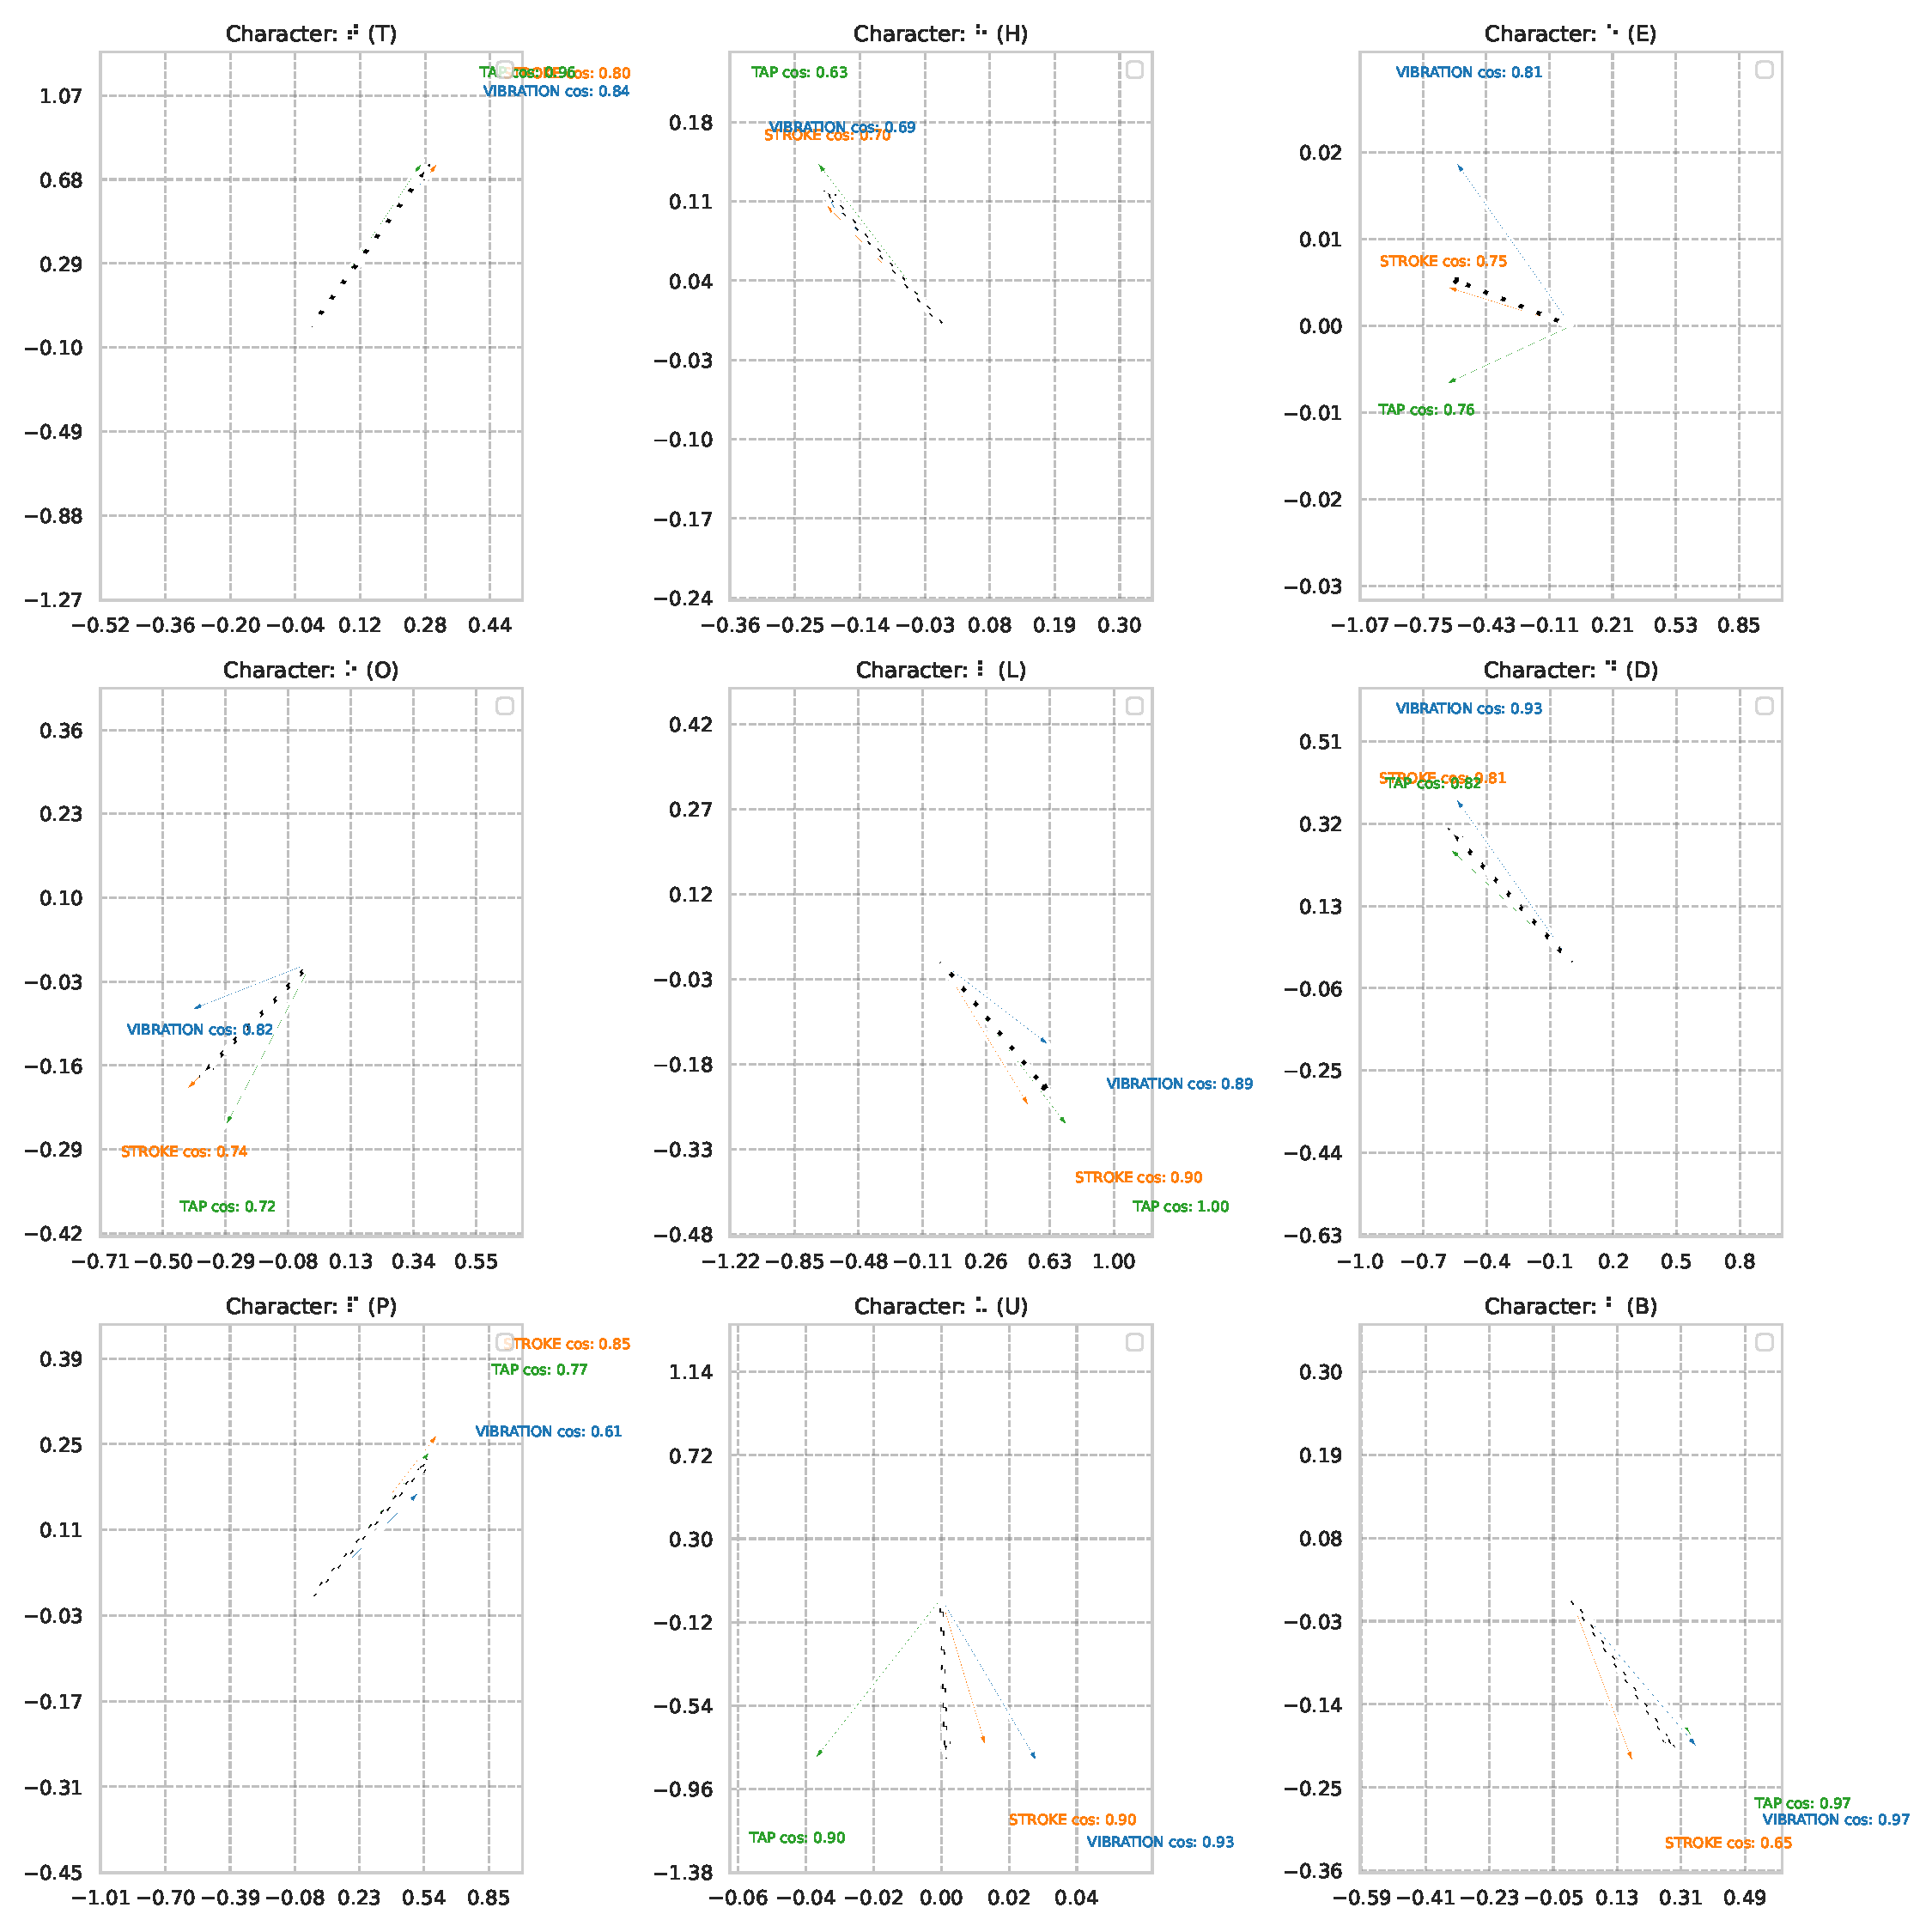
\includegraphics[width=\linewidth]{src/pictures/Study1Data_Experiment/Vectors_study1.pdf}
    \caption{Cosine Similariy for each of the Stimuli.\\Plotted using a \gls{pca} dimensionality reduction.}
    \label{fig:cosSim_PCA_study1}
\end{figure}

Lastly, a one-hot encoding vector was created for the pressed keys for each stimulus, similar to a column in \autoref{fig:missed_surplus_percentages_study1}. 
In order to visually represent the differences between the errors.
We then calculated the cosine similarity for each stimulus character vector embedding against the ground truth, which is depicted by the black dotted line in \autoref{fig:cosSim_PCA_study1}.
To present the cosine similarity in a visually appealing manner, we used \gls{pca} to reduce the dimensionality to two dimensions for plotting.

The cosine similarity and \gls{pca} analysis, as shown in the figure, indicate that despite noise reduction through \gls{pca}, the vectors align in a similar direction. The most noticeable differences were observed for the braille characters \braille{u}(U), \braille{e}(E), and \braille{o}(O).
But their Cosine similarity scores were still very similar with cosine scores of 0.81 (Vibration), 0.76 (Tapping) and 75 (Stroking) for the braille character \braille{e}(E), cosine scores of 0.82 (Vibration), 0.72 (Tapping) and 0.74 (Stroking) for the \braille{o}(O).
And lastly 0.9 (Tapping), 0.93 (Vibration) and 0.9 (Stroking) for the braille character \braille{u}(U)



\subsection{Second Study}

\begin{table}
\resizebox{\columnwidth}{!}{
    \centering
    \begin{tabular}{|c|c|c|c|} \hline 
        Gender & Age & Dominant Hand & Previous Braille Knowledge\\ \hline 
        F & 21 & R & No\\ \hline 
        M & 61 & L & No\\ \hline 
        M & 23 & R & No\\ \hline 
        F & 27 & R & No\\ \hline 
        F & 29 & R & No\\ \hline 
        M & 23 & R & No\\ \hline 
        M & 26 & R & No\\ \hline 
        M & 23 & R & No\\ \hline
    \end{tabular}}
    \caption{Second study participant data}
    \label{tab:study2_participant_data}
\end{table}
\begin{figure}
    \centering
    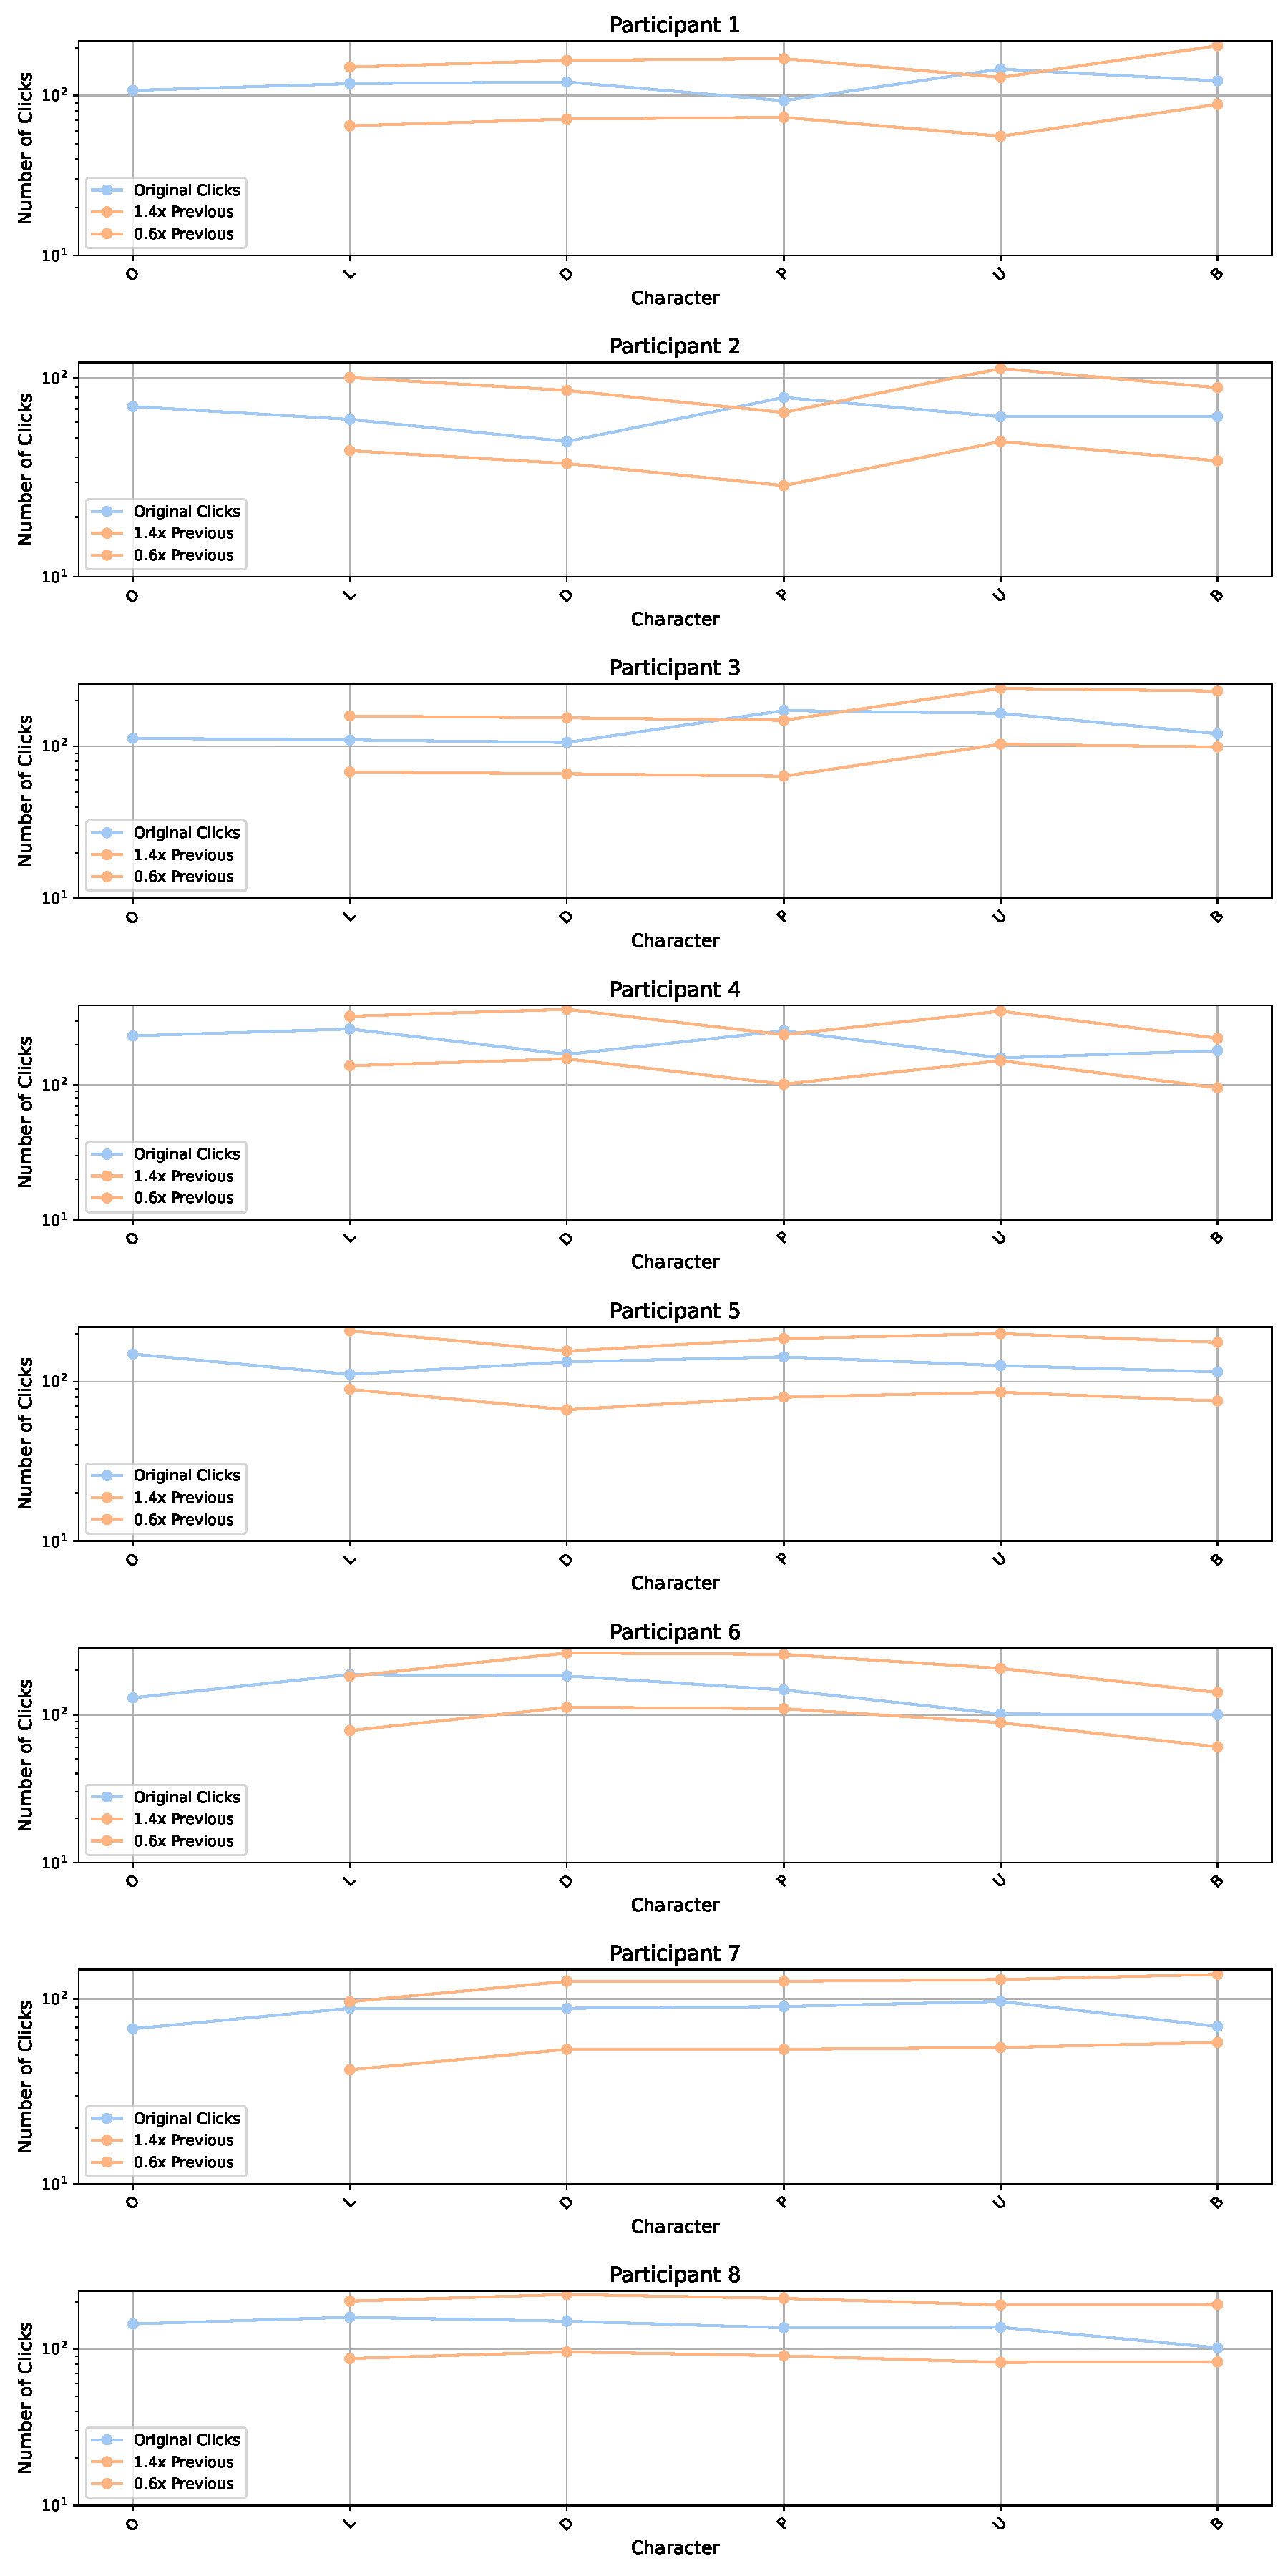
\includegraphics[width=0.5\linewidth]{src/pictures/Study2Data_questionnaire/participantPlots_study2.pdf}
    \caption{Participant Click-differences.}
    \label{fig:participant_clicks-secondStudy}
\end{figure}

For the second study, we interviewed 8 participants (5 male, 3 female) aged between 4 and 61 years, with an average age of 29.125 years and a median age of 24.5 years. Of these, 7 participants were right-handed and 1 was left-handed, as shown in \autoref{tab:study2_participant_data}. None of the participants had prior knowledge of Braille.


\begin{figure}
    \centering
    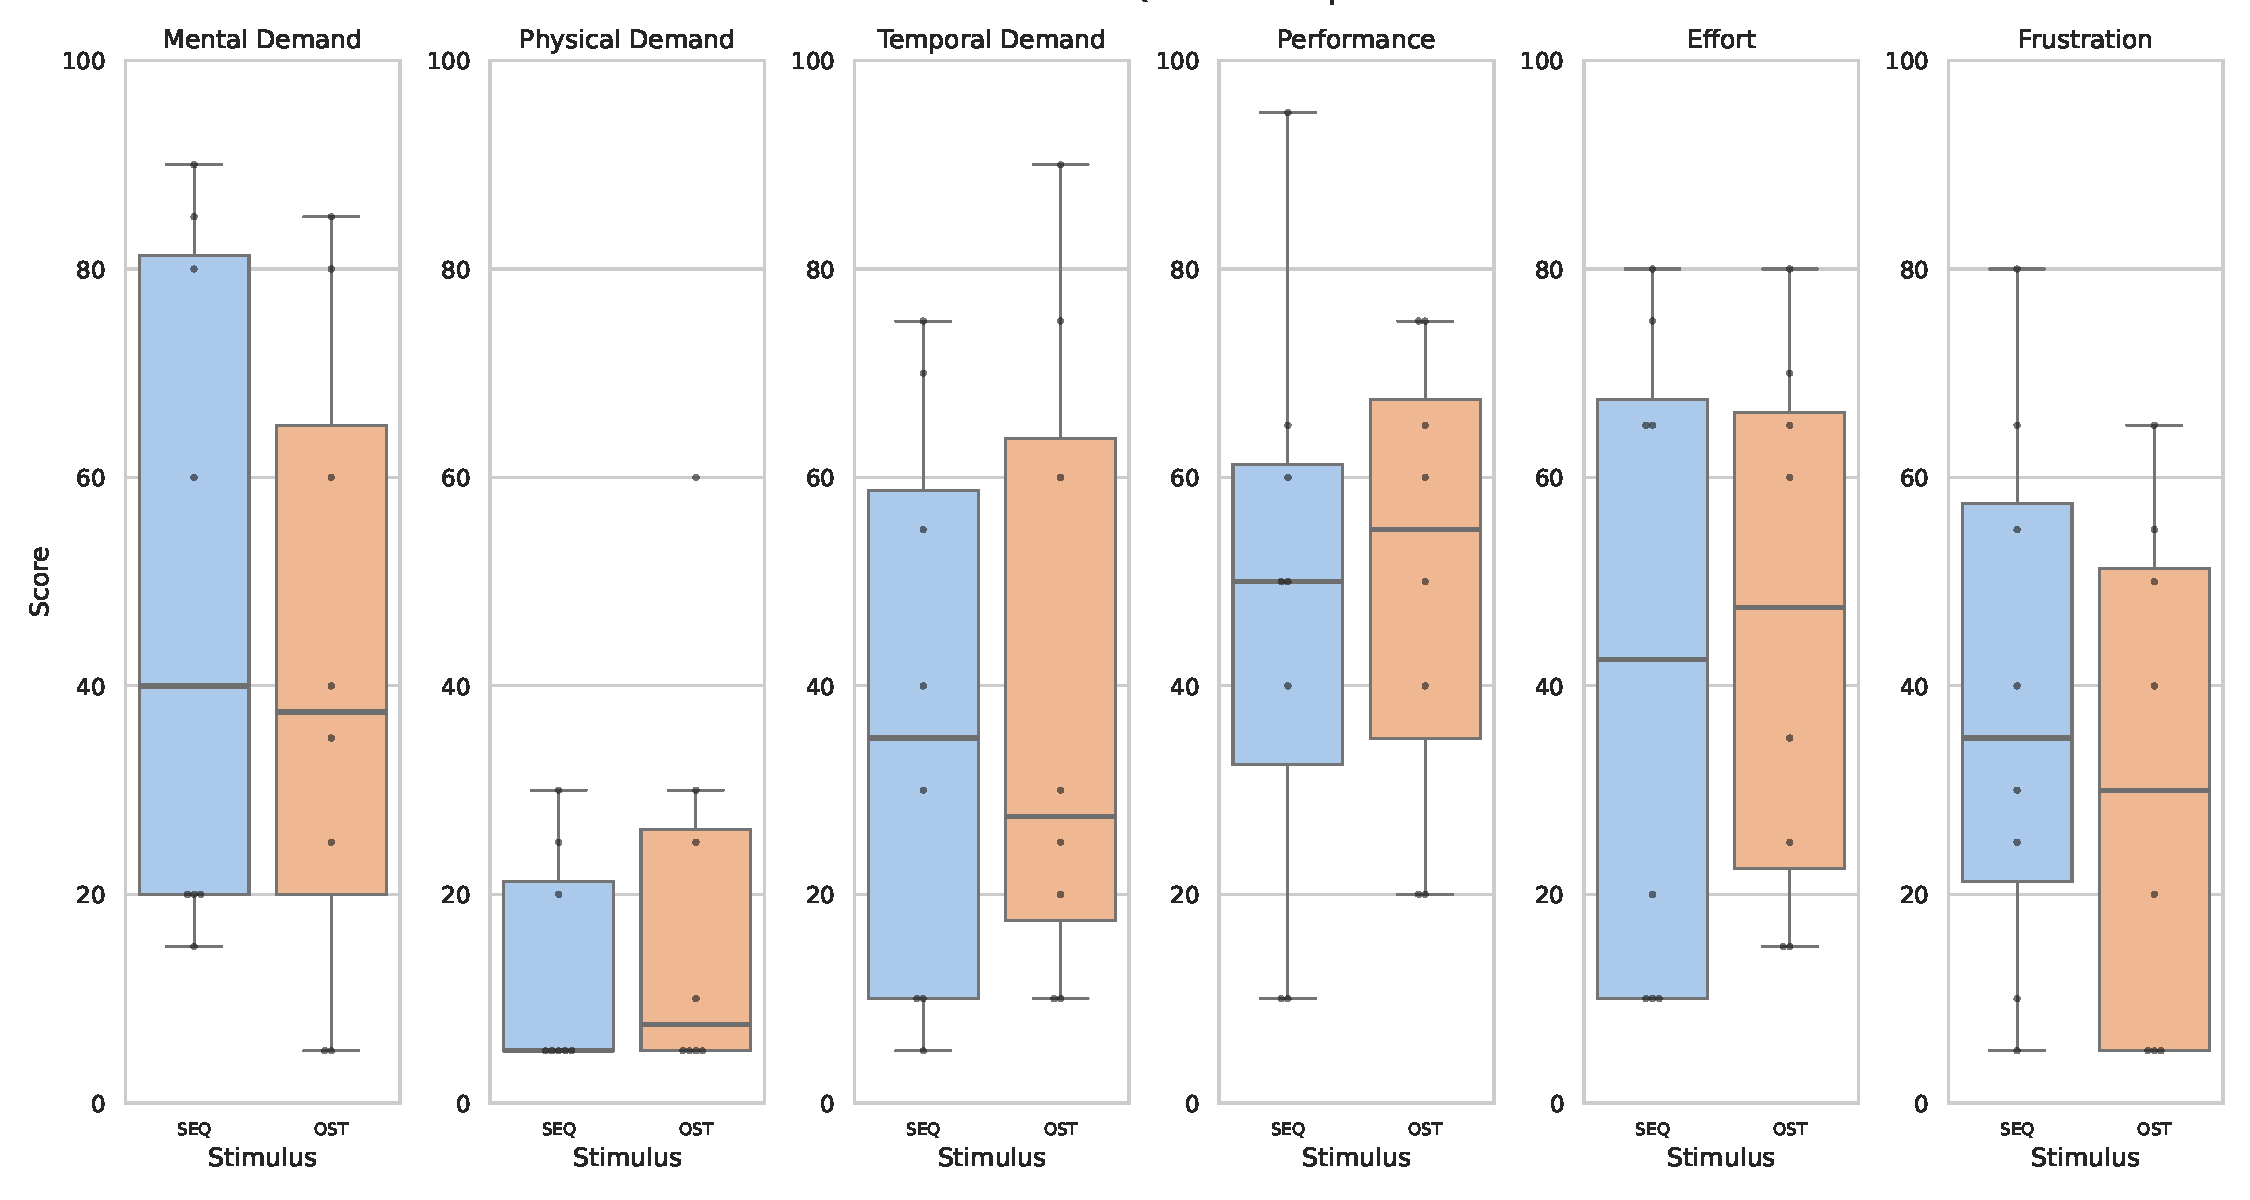
\includegraphics[width=\linewidth]{src/pictures/Study2Data_questionnaire/nasaTLX_study2.pdf}
    \caption{Raw Nasa TLX scores of the different Encodings grouped by the Nasa TLX dimensions.}
    \label{fig:nasaTLX-secondStudy}
\end{figure}

Consistent with the first study, we conducted a NASA TLX test after each encoding sequence to assess the task load experienced by the participants. The results of the NASA TLX are presented in \autoref{fig:nasaTLX-secondStudy}, where each encoding is displayed as a box plot grouped by the NASA TLX dimensions.

As shown, the respective box plots for the dimensions appear similar, with medians of $40$ for \gls{seq} and $35$ for \enquote{ost} under the \enquote{Mental Demand} category. The Q1-Q3 quantiles for \gls{seq} range from $20$ to $82$, while for \enquote{ost}, they range from $20$ to $65$.

For the \enquote{Physical Demand} category, the median for \gls{ost} is slightly lower at $5$, compared to the median of approximately $7.5$ for \gls{seq}. The Q1-Q3 quantiles start at $5$ for both encodings, but \gls{seq} extends up to $22.5$, while \enquote{ost} reaches $25$.

In the \enquote{Temporal Demand} category, the medians are $35$ for \gls{seq} and $30$ for \enquote{ost}, with similar quantile ranges—$10$ to $57.5$ for \gls{seq} and $17.5$ to $65$ for \enquote{ost}.

Similar to the previous categories, the median for \gls{seq} in the \enquote{Frustration} category is higher, at $35$, compared to the median of $30$ for \enquote{ost}.

For the \enquote{Performance} and \enquote{Effort} categories, the medians show a similar trend. The median for \gls{seq} is $50$ in the \enquote{Performance} category, while \enquote{ost} has a median of $55$. For \enquote{Effort}, the median for \gls{seq} is $42.5$, whereas \enquote{ost} has a median of $47.5$.

To assess the significance of the NASA TLX results, we conducted \gls{mwu} significance tests, with the outcomes presented in \autoref{table:nasaTLX_significance_secondStudy_nonParam}. As shown, all p-values are relatively high, indicating that the null hypothesis ($H_0$) was not rejected.

\begin{table}[ht]
\resizebox{\columnwidth}{!}{
\centering
\begin{tabular}{|l|l|l|l|l|}
\hline
\textbf{Question} & \textbf{Test Statistic} & \textbf{p-value}  &\textbf{Significance}           &\textbf{Effect Size}\\ \hline
\textbf{Mental Demand}        & 35.500& 0.7513&Not Significant &0.2141\\ \hline
\textbf{Physical Demand}      & 27.000& 0.6019&Not Significant &0.3559\\ \hline
\textbf{Temporal Demand}      & 29.0000& 0.7911&Not Significant &0.1065\\ \hline
 \textbf{Performance}          & 27.5000& 0.6721&Not Significant &0.1228\\\hline
 \textbf{Effort}               &  27.500& 0.672&Not Significant &0.1285\\\hline
 \textbf{Frustration}          & 39.0000& 0.4907&Not Significant &0.3168\\\hline
\end{tabular}}
\caption{Results of \gls{mwu} significance tests for the different NasaTLX dimensions with Cohens d.}
\label{table:nasaTLX_significance_secondStudy_nonParam}
\end{table}

\begin{figure}
    \centering
    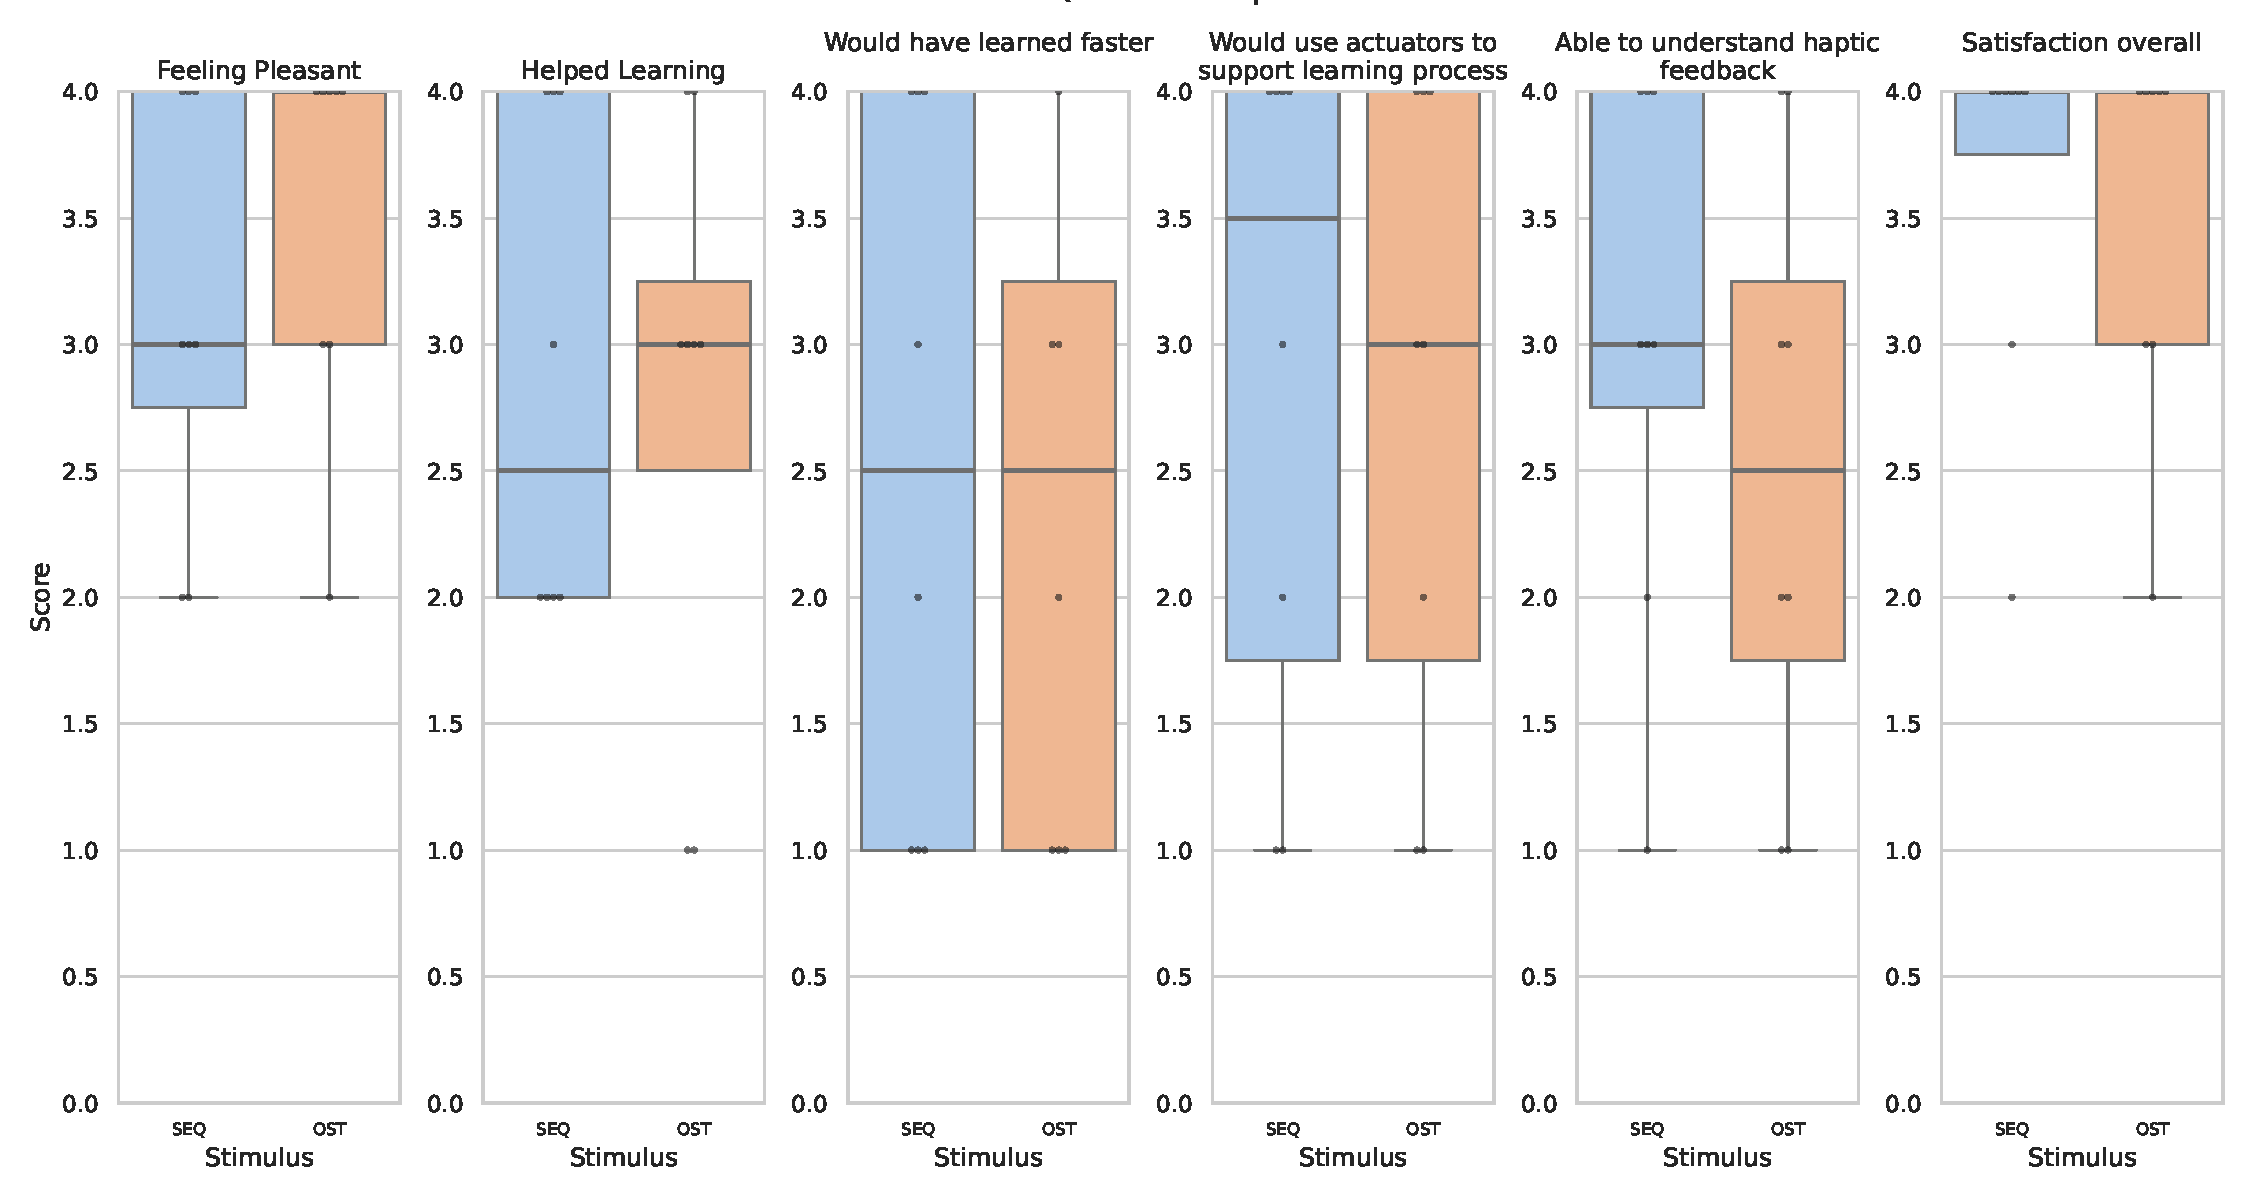
\includegraphics[width=\linewidth]{src/pictures/Study2Data_questionnaire/questions_special_study2.pdf}
    \caption{Self-assessment Results of the different Stimuli grouped by the self-assessment categories.}
    \label{fig:questions_individual_secondStudy}
\end{figure}

Following the NASA TLX task load, participants were asked to evaluate their experiences with the two different encodings. Their evaluations were plotted across six different dimensions, as shown in \autoref{fig:questions_individual_secondStudy}.

The largest differences in medians were observed in the categories: \enquote{Helped Learning}, with medians of $2.5$ for \gls{seq} and $3$ for \gls{ost}; \enquote{Would use actuators to support the learning process}, with $3.5$ for \gls{seq} and $3$ for \gls{ost}; \enquote{Able to understand haptic feedback}, with $3$ for \gls{seq} and $2.5$ for \gls{ost}; and \enquote{Satisfaction overall}, with $3.75$ for \gls{seq} and $3$ for \gls{ost}. 

The medians for the categories \enquote{Feeling Pleasant} ($3$) and \enquote{Would have learned faster} ($2.5$) were the same for both encodings. 

The Q1-Q3 quantile ranges differed notably in the \enquote{Helped Learning} category, where \gls{seq} ranged from $2$-$4$ and \gls{ost} from $2.5$-$3.25$. In \enquote{Satisfaction overall}, the difference was also noticeable, with \gls{seq} ranging from $3.75$-$4$ and \gls{ost} from $3$-$4$. 

For the \enquote{Would have learned faster} category, the quantile ranges showed a significant difference, with \gls{seq} and \gls{ost} both starting at Q1 = $1$, but \gls{seq} extending to $4$ and \gls{ost} to $3$. 

Finally, the quantile ranges for the \enquote{Able to understand haptic feedback} dimension were nearly identical, with \gls{seq} ranging from $2.75$-$4$ and \gls{ost} from $1.75$-$3.25$.

For the self-assessment tests, we also conducted \gls{mwu} significance tests, and the results are presented in \autoref{table:individualQuestions_significance_secondStudy_nonPara}.
The lowest p-value was found for the \enquote{Feeling Pleasant} dimension; however, with a p-value of $0.3596$, it remains too high to indicate statistical significance.
Therefore, there is no significant difference between the two encodings in terms of self-assessment for usability and their effectiveness in aiding learning.

\begin{table}[ht]
\resizebox{\columnwidth}{!}{
\centering
\begin{tabular}{|l|l|l|l|l|}
\hline
\textbf{Question} & \textbf{U-statistic}& \textbf{p-value}  &\textbf{Significance}           &\textbf{Effect Size}\\ \hline
\textbf{Feeling Pleasant}& 23.5000& 0.3596&Not Significant &0.2232\\ \hline
\textbf{Helped Learning}& 33.0000& 0.9565&Not Significant &0.0263\\ \hline
\textbf{Would have learned faster}& 32.5000& 1.000&Not Significant &0.0131\\ \hline
 \textbf{Would use actuators to support learning process}& 34.5000& 0.8244&Not Significant &0.0656\\\hline
 \textbf{Able to understand haptic feedback}&  40.0000& 0.4139&Not Significant &0.2100\\\hline
 \textbf{Satisfaction overall}& 35.5000& 0.7001&Not Significant &0.0919\\\hline
\end{tabular}}
\caption{Results of the \gls{mwu} test for significance grouped by the different self-assessment dimensions with a Cohens d Effect Size.}
\label{table:individualQuestions_significance_secondStudy_nonPara}
\end{table}

\begin{figure}
    \centering
    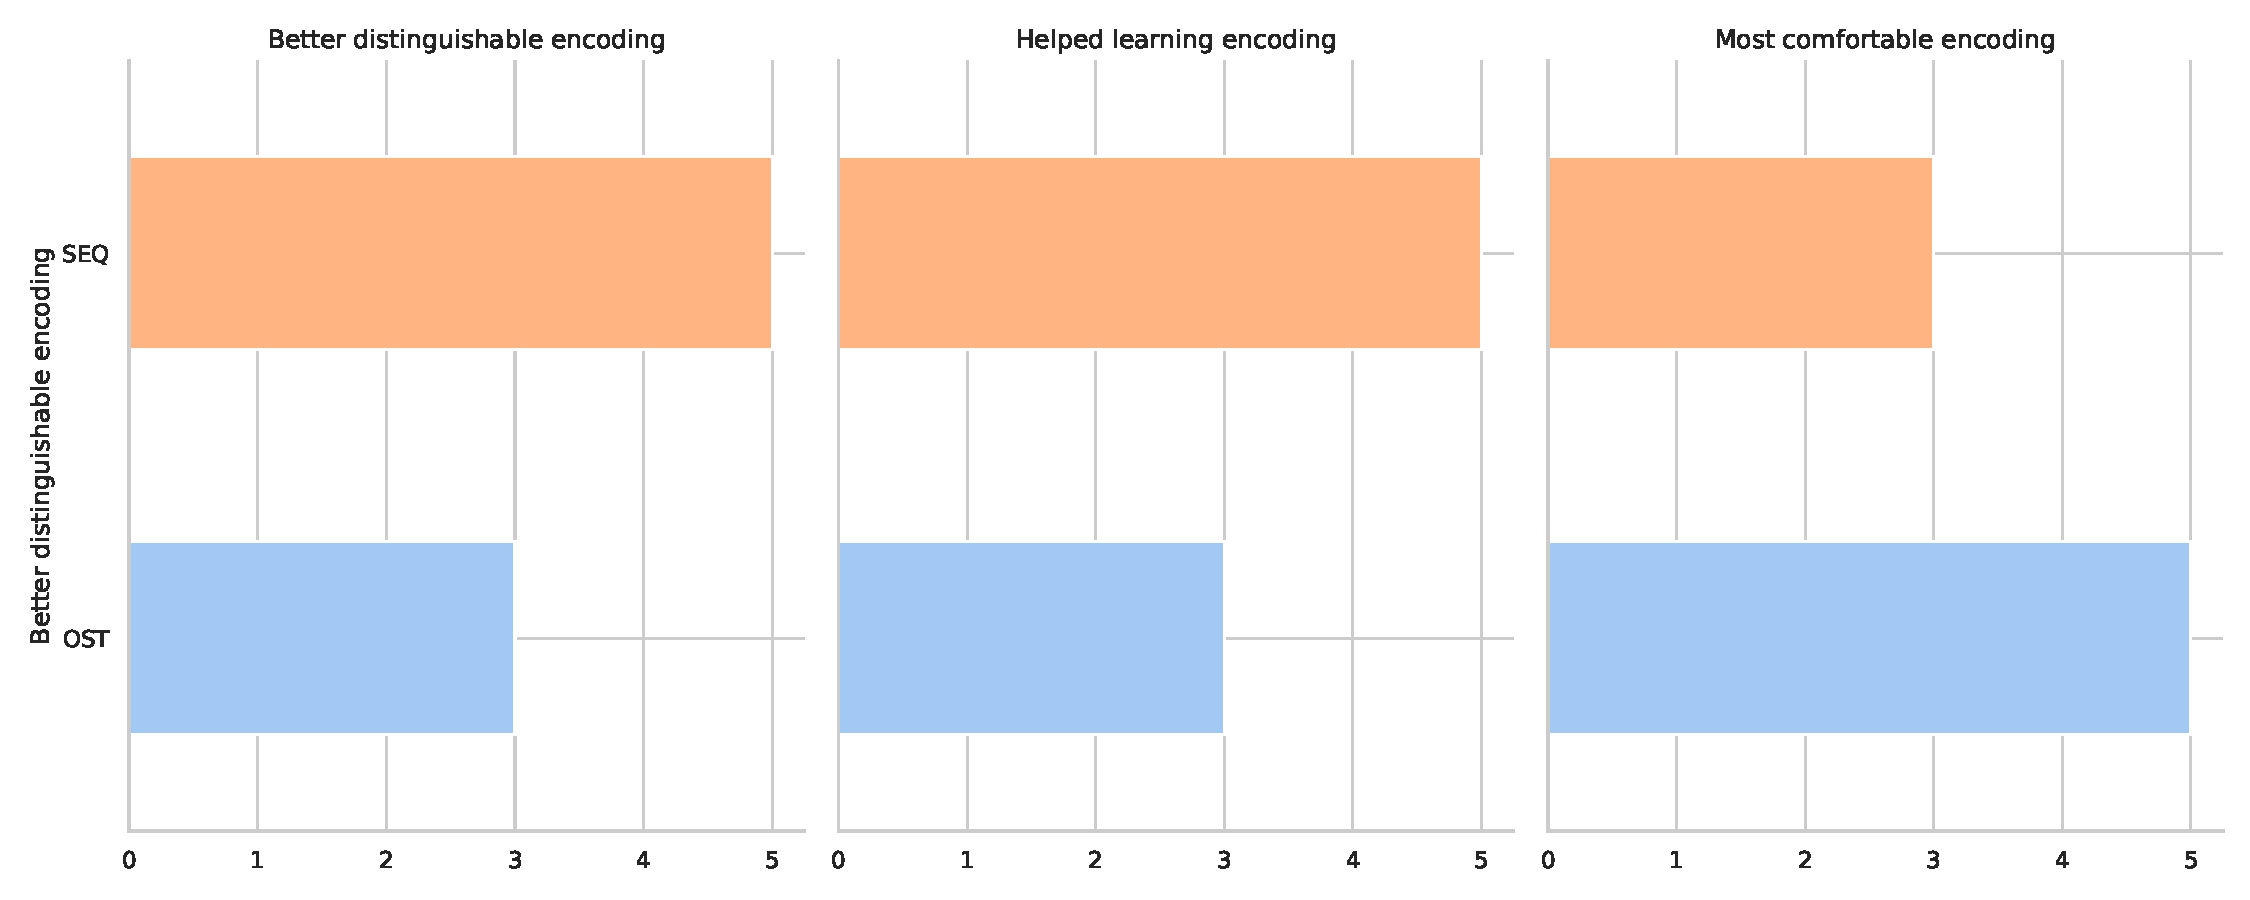
\includegraphics[width=\linewidth]{src/pictures/Study2Data_questionnaire/questions_compare_study2.pdf}
    \caption{Results of the direct comparison between the different encodings.}
    \label{fig:questionsCompare-secondStudy}
\end{figure}

After the study, we asked the participants to compare the two encoding methods, and the results are presented in \autoref{fig:questionsCompare-secondStudy}.
The comparison reveals that the \gls{seq} encoding was perceived as more distinguishable, with $62.5\%$ of participants agreeing, and it was also considered more helpful for learning with the same proportion.
However, the \gls{ost} encoding was regarded as more comfortable, with $62.5\%$ of participants reporting it as more comfortable than the \gls{seq} encoding.

A statistical analysis, presented in \autoref{table:statistical_tests_comparrisson_secondStudy}, showed that conducting the \gls{csgf} study resulted in no significant difference.
The \gls{csgf} was chosen due to insufficient data for a Chi-Squared test.

\begin{table}
\resizebox{\columnwidth}{!}{
    \centering
    \begin{tabular}{|c|c|c|c|}\hline
        Question & \gls{csgf} & p-value & Significance \\\hline
         \enquote{Better distinguishable encoding} & 0.5 & 0.4795& Not Significant\\\hline
         \enquote{Helped Learning encoding} & 0.5 & 0.4795 & Not Significant\\\hline
         \enquote{Most comfortable encoding}& 0.5 & 0.4795 & Not Significant\\\hline
    \end{tabular}}
    \caption{Statistical \gls{csgf} Results for the direct comparison between the stimuli.}
    \label{table:statistical_tests_comparrisson_secondStudy}
\end{table}




\begin{figure}
    \centering
    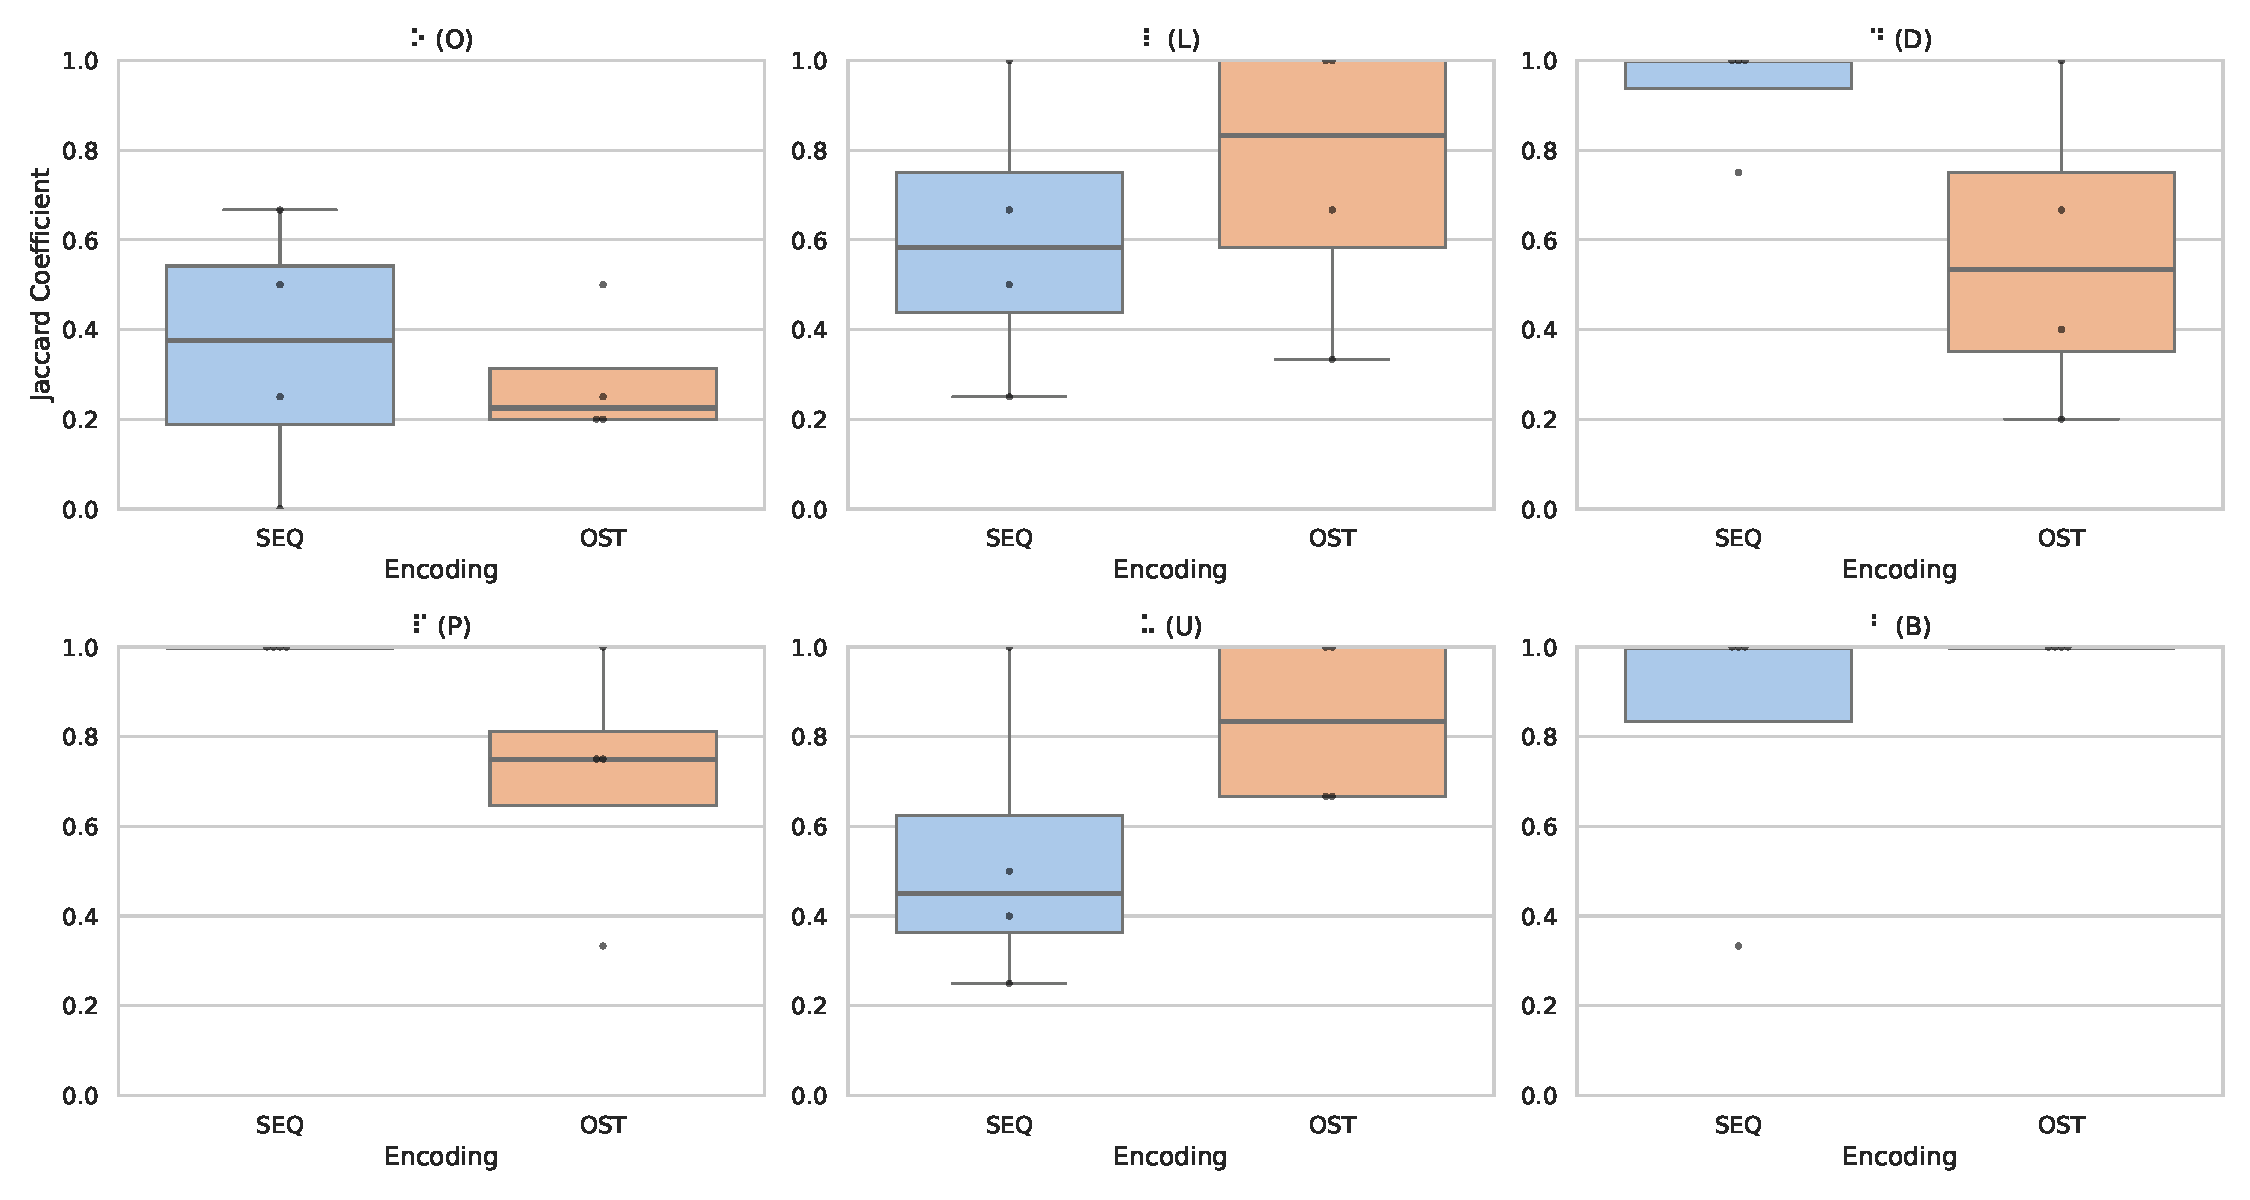
\includegraphics[width=\linewidth]{src/pictures/Study2Data_Experiment/study2_learning_results.pdf}
    \caption{Jaccard coefficient results grouped by the Braille characters during learning for the different Encodings.}
    \label{fig:learning_results_secondStudy}
\end{figure}

During the learning process, we measured performance using the Jaccard and Dice scores. The Jaccard results after learning each character are shown in \autoref{fig:learning_results_secondStudy}, as they are more stringent than the Dice scores.

The charts reveal larger differences in the medians for \braille{d}(D), with a median of $0.95$ for \gls{seq} and $0.55$ for \gls{ost}.
Similarly, for the \braille{u}(U) test, the median difference is substantial, with \gls{seq} showing a median of about $0.45$ and \gls{ost} performing better with a median of $0.825$.
\gls{ost} also outperformed \gls{seq} for the character \braille{l}(L), with a median of $0.825$ compared to $0.575$ for \gls{seq}.
For the character \braille{b}(B), \gls{ost} showed better performance, with a median of $1$, which was consistent across the Q1 and Q3 quantiles. In comparison, \gls{seq} had a median of $0.825$, with Q1 equal to that value and Q3 at $1$.
However, for the character \braille{p}(P), \gls{seq} performed better, with a median, Q1, and Q3 of $1$, compared to \gls{ost}, which had a median of $0.75$, Q1 of $0.65$, and Q3 of $0.82$.

Afterwards, we conducted the appropriate \gls{mwu} tests for significance, and the results are shown in \autoref{table:learning_significance_results_secondStudy_nonPar_learning}.
However, none of the tests showed statistically significant differences.
The lowest p-value was observed in the \braille{b}(B) test, with a value of $0.067$, which also had a Cohen's d effect size of $1.492$, indicating a relatively large effect.

\begin{table}[ht]
\resizebox{\columnwidth}{!}{
\centering
\begin{tabular}{|l|l|l|l|l|}
\hline
\textbf{Question} & \textbf{Test Statistic} & \textbf{p-value}  &\textbf{Significance}           &\textbf{Effect Size}\\ \hline
\braille{o}(\textbf{O})& 10.000& 0.659&Not Significant &0.290\\ \hline
\braille{l}(\textbf{L})& 5.500& 0.552&Not Significant &0.460\\ \hline
\braille{d}(\textbf{D})& 13.500& 0.124&Not Significant &1.424\\ \hline
\braille{p}(\textbf{P})& 14.000& 0.067&Not Significant &1.492\\ \hline
\braille{u}(\textbf{U})& 3.000& 0.180&Not Significant &1.108\\ \hline
\braille{b}(\textbf{B})& 6.000& 0.453&Not Significant &0.707\\ \hline
\end{tabular}}
\caption{Results of the \gls{mwu} tests for significance grouped by the different Braille characters during training for the different Encodings with Cohen's d.}
\label{table:learning_significance_results_secondStudy_nonPar_learning}
\end{table}

\begin{figure}
    \centering
    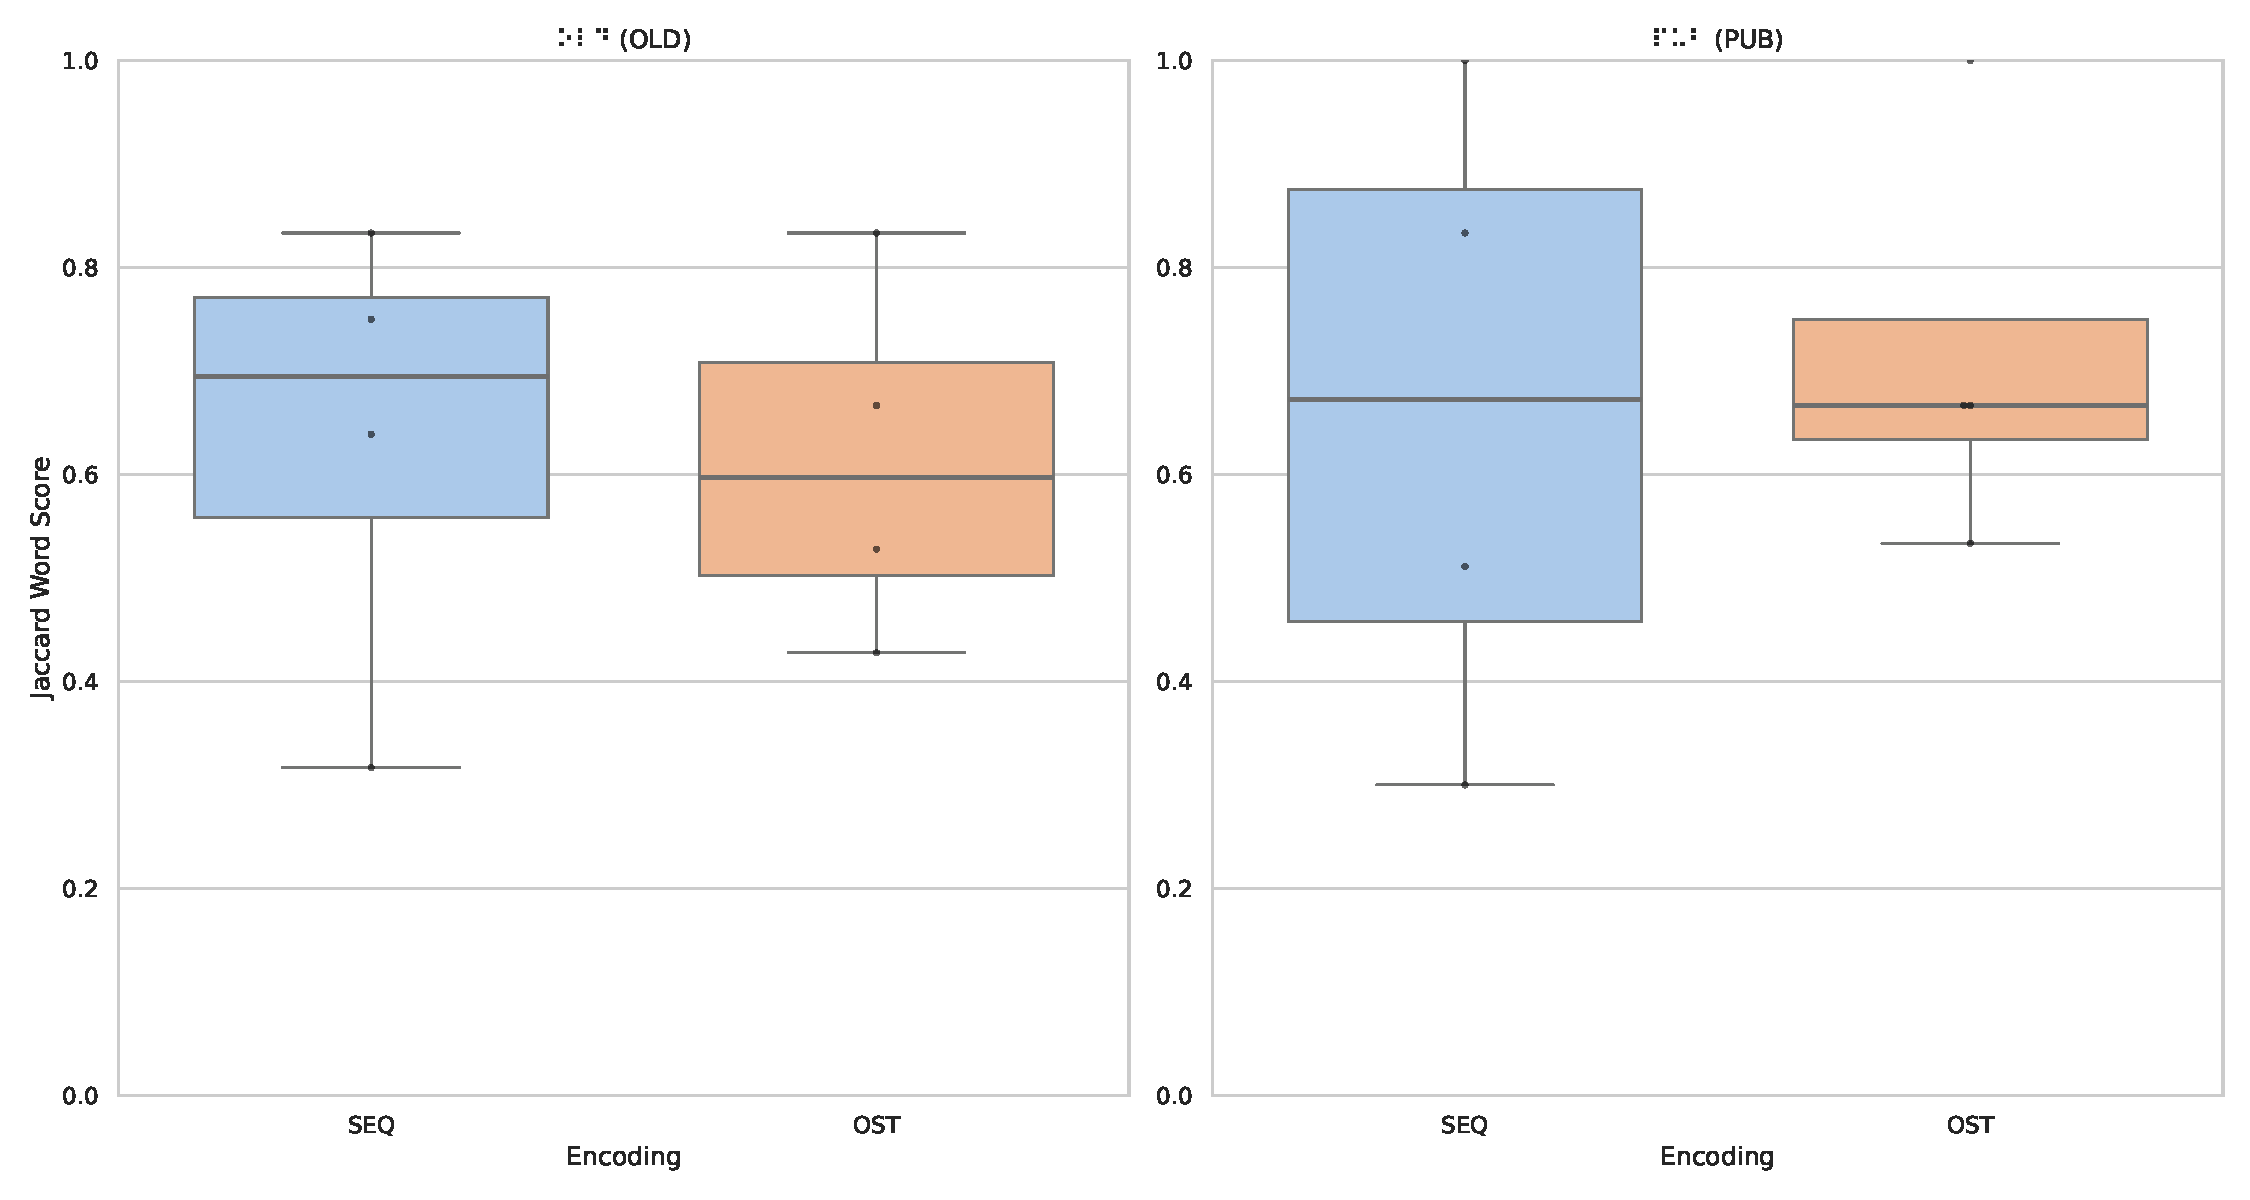
\includegraphics[width=\linewidth]{src/pictures/Study2Data_Experiment/study2_test_results.pdf}
    \caption{Jaccard Word-Test results grouped by the Braille test-words for the different stimuli.}
    \label{fig:study2_test_results-firstStudy}
\end{figure}

After learning each word using one of the encodings, we tested the word itself, with the results shown in \autoref{fig:study2_test_results-firstStudy}, to determine whether there was a significant difference in testing the entire word after learning all the individual characters.
Interestingly, no significant difference was observed in the median. However, the Q1 and Q3 values for the word "pub" differed, with an interval of $0.62$-$0.85$ for \gls{ost} compared to $0.45$-$0.875$ for \gls{seq}.
Nevertheless, the median remained the same for both encodings, at $0.675$.

We conducted \gls{mwu} tests for the resulting words, and the results showed that no p-value was close to the threshold value of $0.05$, as depicted in \autoref{table:significance_results_test_secondStudy_nonPara}. This indicates that there was no significant difference between the sets, with p-values of $1.0$ and $0.77$.

\begin{table}[ht]
\resizebox{\columnwidth}{!}{
\centering
\begin{tabular}{|l|l|l|l|l|}
\hline
\textbf{Question} & \textbf{Test Statistic} & \textbf{p-value}  &\textbf{Significance}           &\textbf{Effect Size}\\ \hline
\braille{old}(\textbf{OLD})& 8.500& 1.000&Not Significant &0.103\\ \hline
\braille{pub}(\textbf{PUB})& 6.500& 0.770&Not Significant &0.211\\\hline
\end{tabular}}
\caption{Results of the \gls{mwu} tests for significance for the different Braille tests-words with a Cohens d Effect Size.}
\label{table:significance_results_test_secondStudy_nonPara}
\end{table}


\begin{figure}
    \centering
    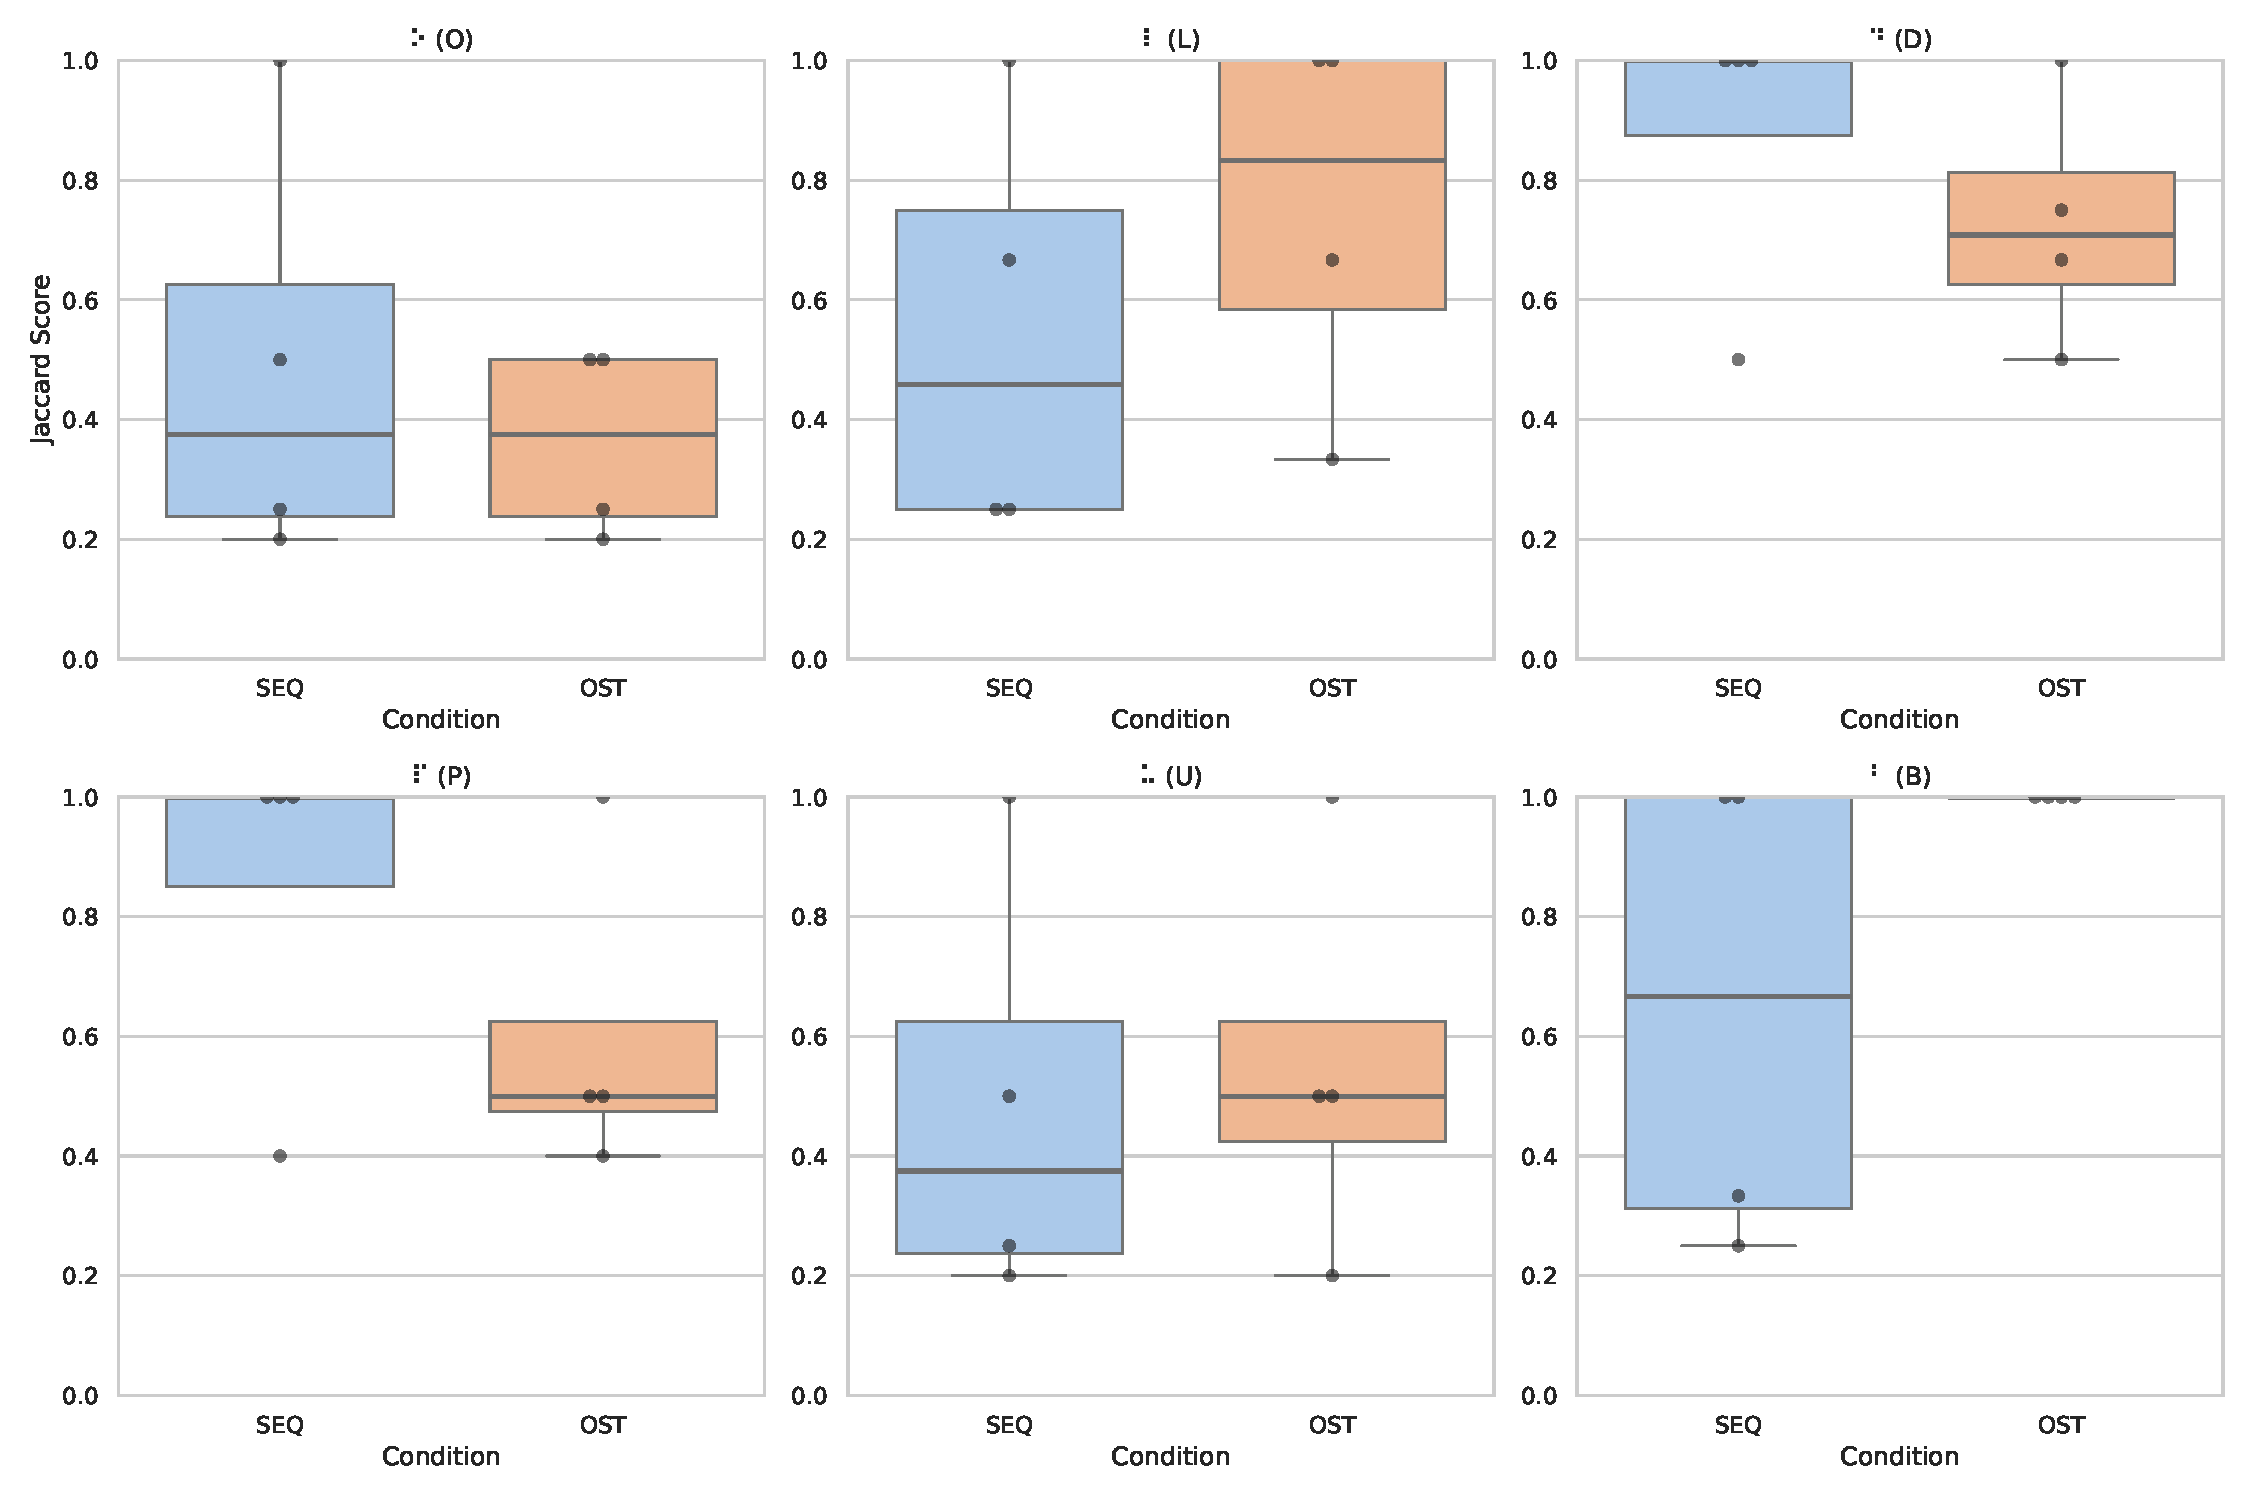
\includegraphics[width=\linewidth]{src/pictures/Study2Data_Experiment/character_jaccard_test_study2.pdf}
    \caption{Jaccard Score comparison for the different Encodings grouped by Braille character.}
    \label{fig:f1score_test_study2}
\end{figure}


\begin{table}[ht]
\resizebox{\columnwidth}{!}{
\centering
\begin{tabular}{|l|l|l|l|l|}
\hline
\textbf{Question} & \textbf{Test Statistic} & \textbf{p-value}  &\textbf{Significance}           &\textbf{Effect Size}\\ \hline
\braille{o}(\textbf{O})& 9.000& 0.881&Not Significant &0.443\\ \hline
\braille{l}(\textbf{L})& 4.500& 0.369&Not Significant &0.609\\ \hline
\braille{d}(\textbf{D})& 11.000& 0.439&Not Significant &0.634\\ \hline
\braille{p}(\textbf{P})& 11.000& 0.436&Not Significant &0.875\\ \hline
\braille{u}(\textbf{U})& 7.000& 0.881&Not Significant &0.179\\ \hline
\braille{b}(\textbf{B})& 4.000& 0.186&Not Significant &1.221\\ \hline
\end{tabular}}
\caption{Results of the \gls{mwu} for significance grouped by the different Braille characters during learning for the different Encodings with Cohen's d.}
\label{table:learning_significance_results_secondStudy_nonPar}
\end{table}

Similarly to the first study, we analyzed the Jaccard scores for the different characters in the second study. The most significant differences were observed for the characters \braille{b}(B), followed by \braille{p}(P), \braille{l}(L), and \braille{d}(D).

For the character \braille{b}(B), the \gls{ost} encoding performed better, achieving a perfect score, while the \gls{seq} encoding had a median of $0.675$ and a Q1-Q3 quantile range of approximately $0.3$ to $1$, as half of the participants did not achieve a perfect score.

In contrast, for the character \braille{p}(P), the \gls{ost} encoding performed worse, with a median around $0.5$, while \gls{seq} had a median of $1$. Similarly, for the character \braille{d}(D), the \gls{seq} encoding had a median of $1$, while \gls{ost} had a median of $0.7$. Notably, only one participant in the \gls{seq} group did not achieve a perfect score, with a score of $0.4$.

It is also worth noting that only one participant had a non-perfect score for \braille{d}(D) using the \gls{seq} encoding.

For the character \braille{l}(L), the \gls{ost} encoding had a median of approximately $0.825$, with half of the participants achieving a perfect score, whereas the \gls{seq} encoding had a median of about $0.45$.

Upon analyzing each character individually, no significant differences were found between the datasets. The lowest p-value was observed for \braille{b}(B), with a value of $0.186$, which is significantly higher than the threshold value. Therefore, the null hypothesis ($H_0$) cannot be rejected.

\begin{figure}
    \centering
    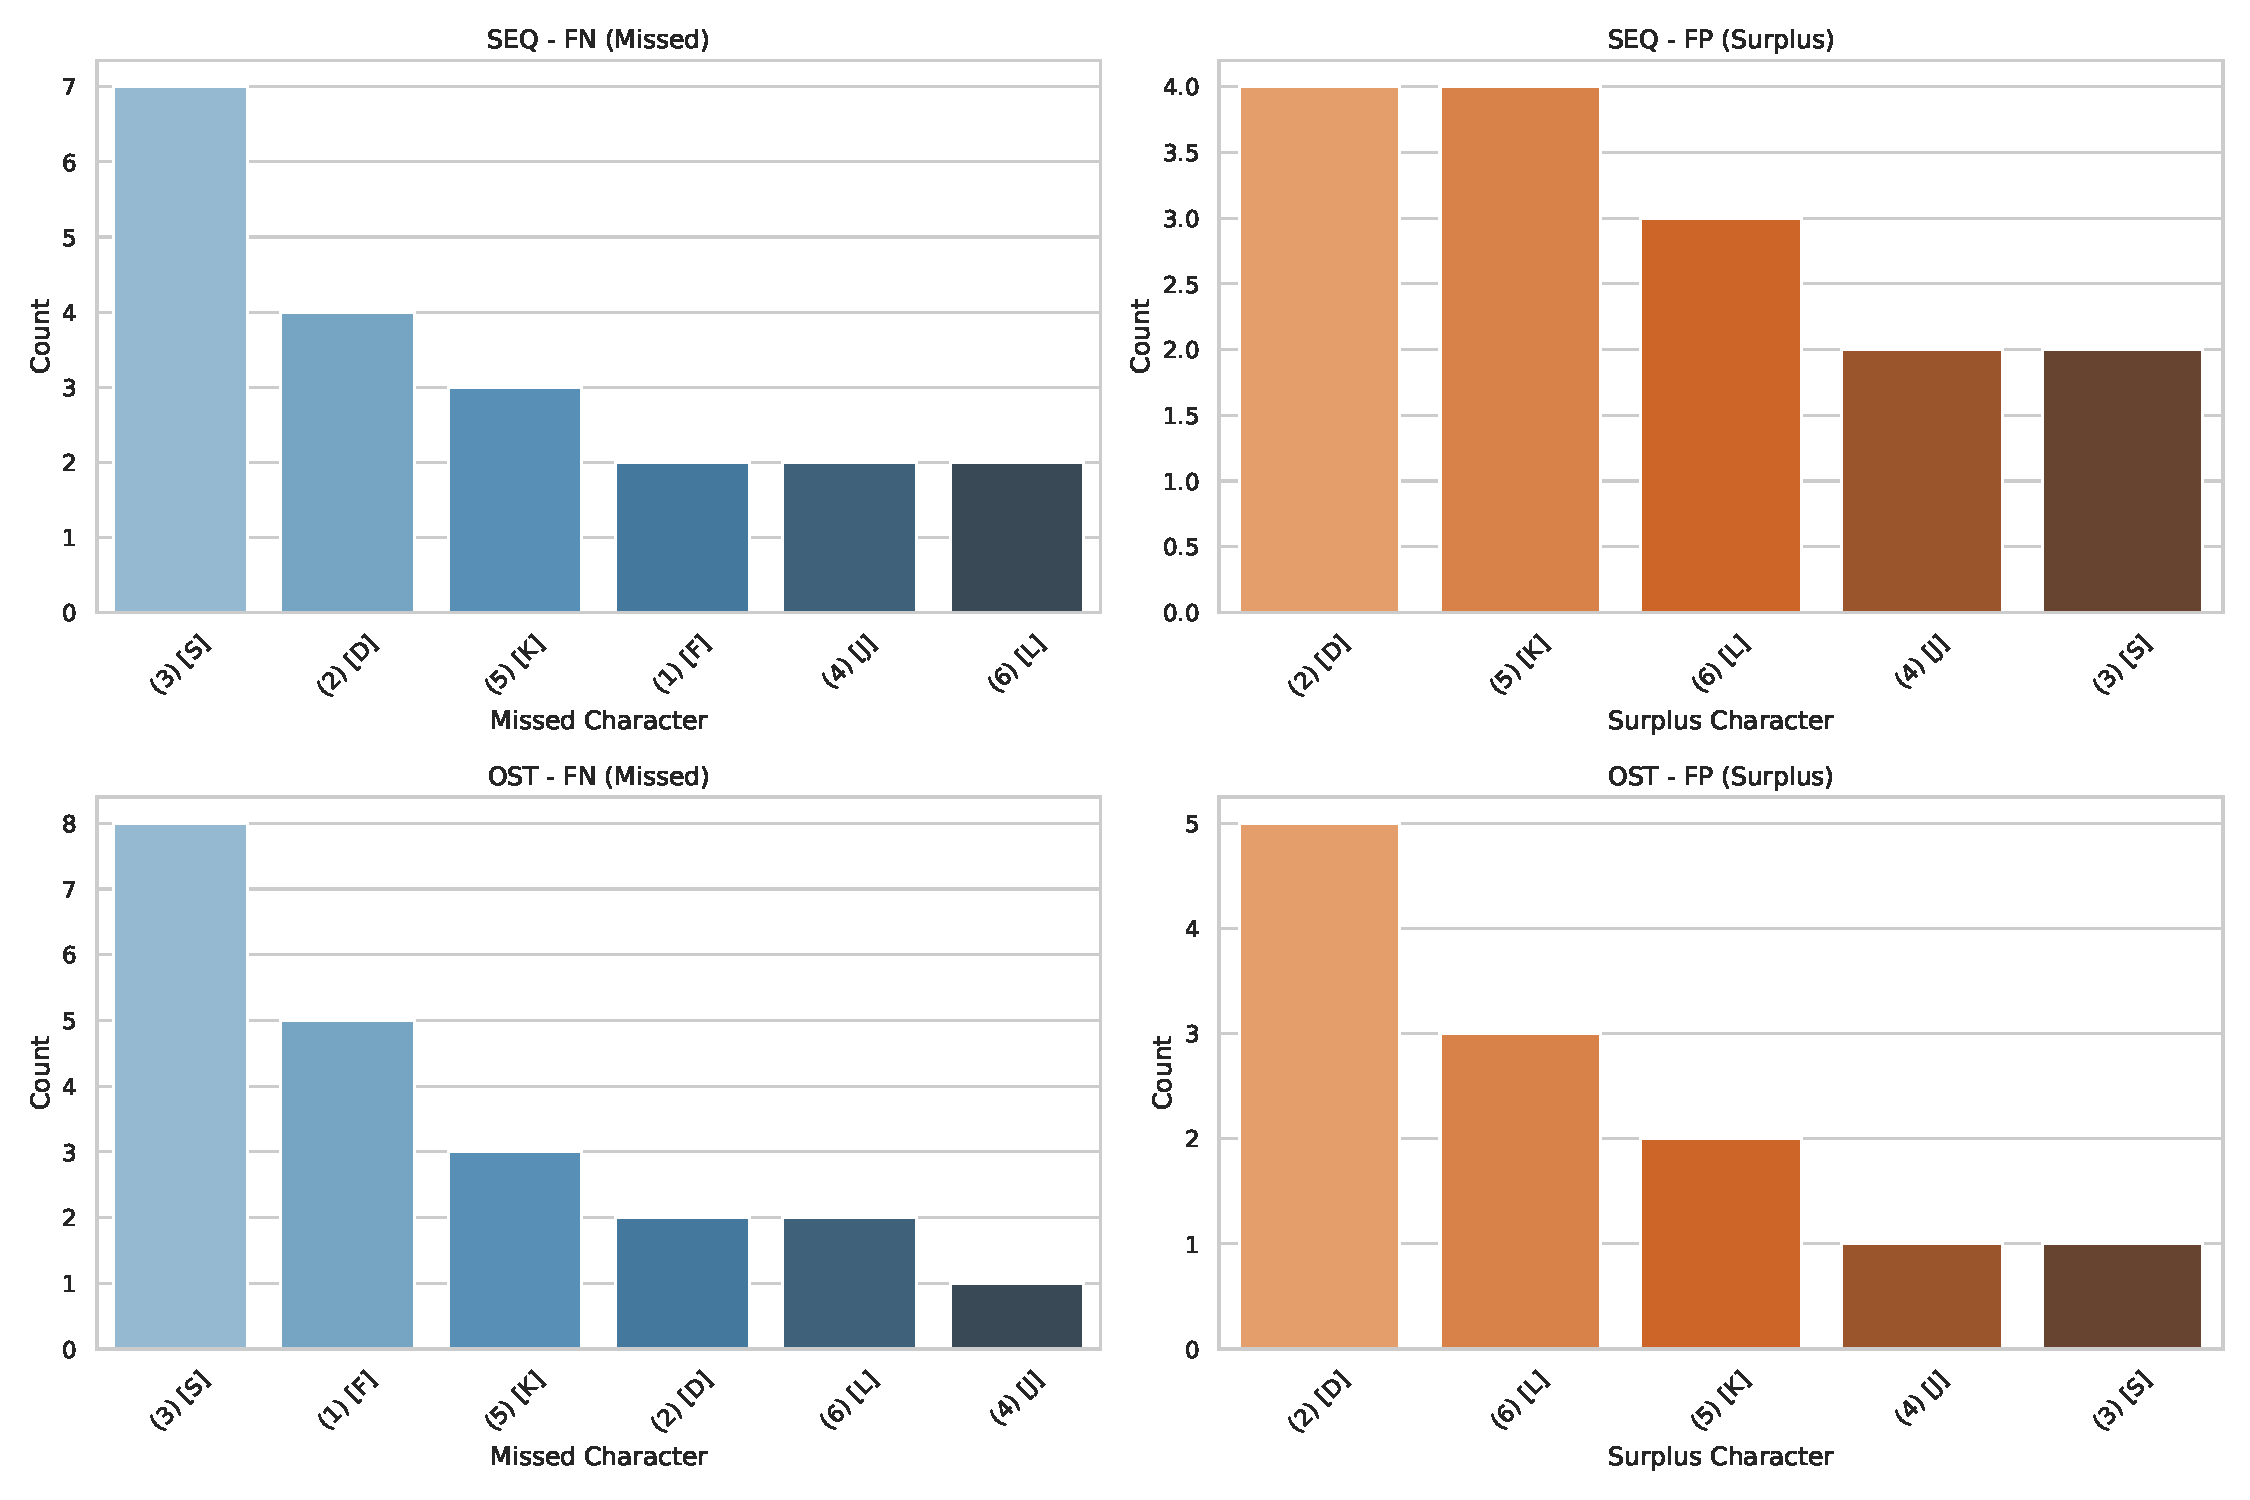
\includegraphics[width=\linewidth]{src/pictures/Study2Data_Experiment/missed_surplus_test_study2.pdf}
    \caption{FN (Missed) and FP (Surplus) Key(s) for each Braille Character by Encoding.}
    \label{fig:missedSurplus_study2}
\end{figure}

Further analysis, shown in \autoref{fig:missedSurplus_study2}, reveals that \textcircled{3} [S] is the most frequently missed character, while \textcircled{2} [D] is the most frequently in surplus. In contrast, \textcircled{4} [J] and \textcircled{6} [L] were the least missed characters, while \textcircled{2} [S] and \textcircled{4} [J] were the least in surplus.

\begin{figure}[h!]
    \centering
    \begin{subfigure}[b]{0.45\textwidth}
        \centering
        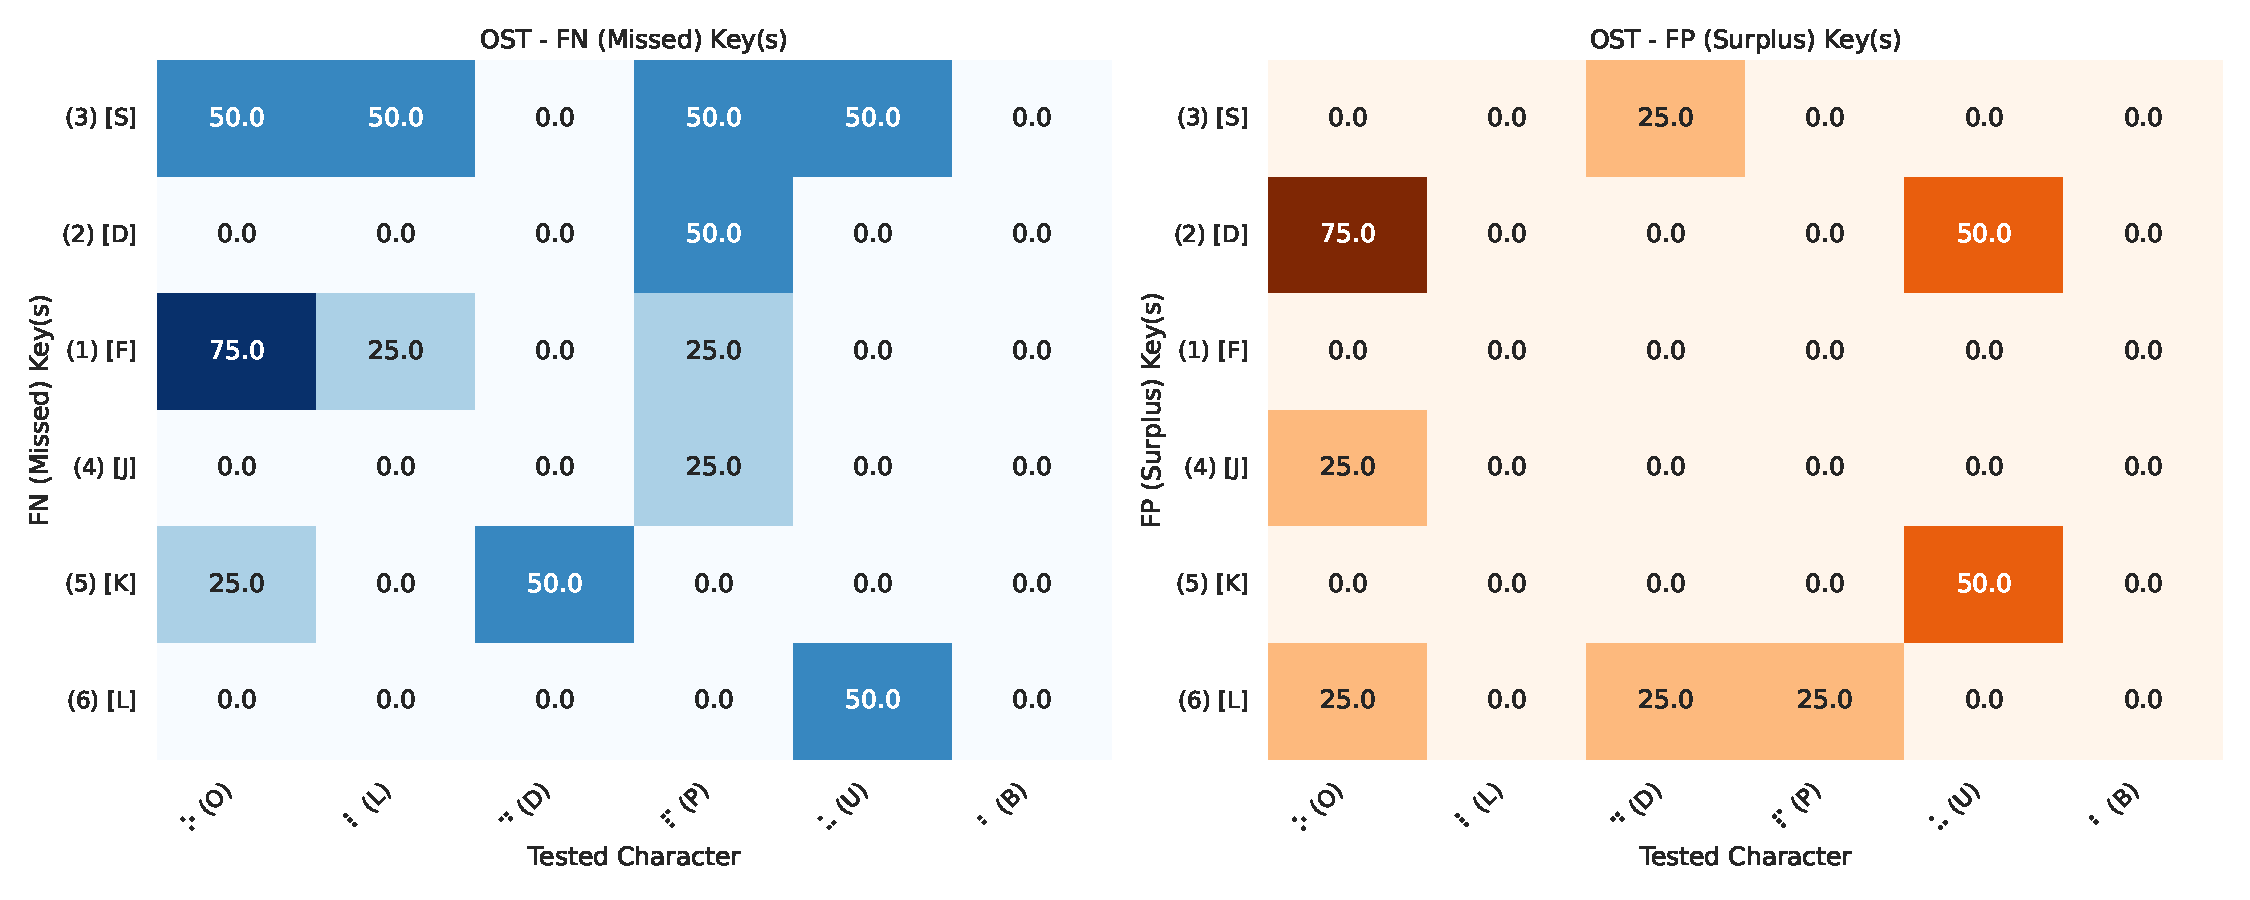
\includegraphics[width=\textwidth]{src/pictures/Study2Data_Experiment/missed_surplus_test_percentages_study2_ost.pdf}
        \caption{\gls{ost}}
    \end{subfigure}
    \begin{subfigure}[b]{0.45\textwidth}
        \centering
        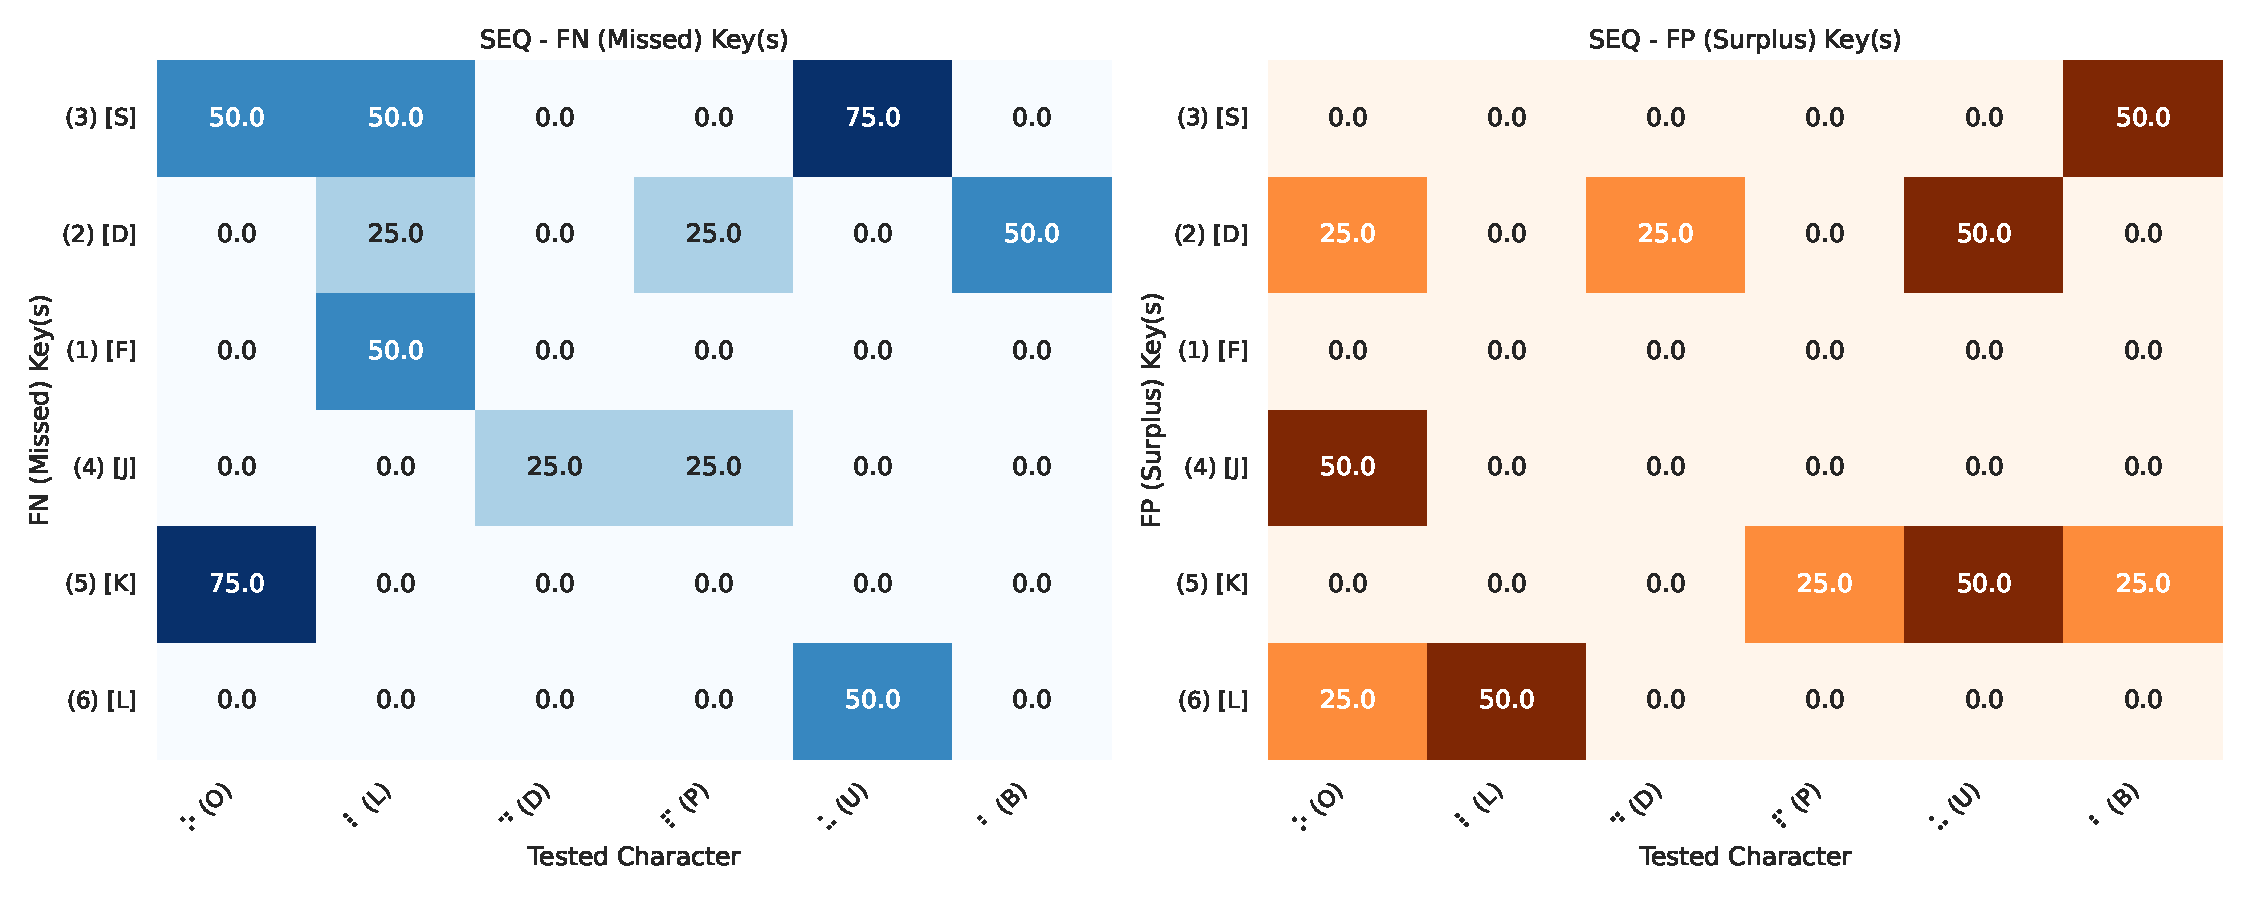
\includegraphics[width=\textwidth]{src/pictures/Study2Data_Experiment/missed_surplus_test_percentages_study2_seq.pdf}
        \caption{\gls{seq}}
    \end{subfigure}\\
    \caption{FN (Missed) and FP (Surplus) Key(s) in percent for each Braille character grouped by Encoding.}
    \label{fig:missed_surplus_percentages_study2}
\end{figure}

A closer analysis reveals that for the false positives (FP), the characters \braille{b}(B), \braille{l}(L), \braille{d}(D), and \braille{p}(P) exhibited the most notable differences.

For \braille{b}(B), the \gls{ost} encoding had no errors, while in the \gls{seq} encoding, the \textcircled{5} [K] and \textcircled{3} [S] keys were mistakenly pressed with the \textcircled{3} [S] key in 50\% of the cases.

For \braille{l}(L), there were no false positives in the \gls{ost} encoding, but half of the participants incorrectly pressed the \textcircled{6} [L] key in the \gls{seq} encoding.

For \braille{d}(D), a larger difference is evident, with 25\% of participants missing \textcircled{3} [S] and \textcircled{6} [L] in the \gls{ost} encoding, while the \textcircled{2} [D] key was incorrectly pressed in the \gls{seq} encoding.

For \braille{p}(P), the \textcircled{6} [L] key was incorrectly pressed in 25\% of the cases in the \gls{ost} encoding, while the \textcircled{5} [K] key was mistakenly pressed in the \gls{seq} encoding.

Regarding the false negatives (FN), the most significant differences were observed for the characters \braille{p}(P), \braille{b}(B), \braille{o}(O), and \braille{l}(L). 

For \braille{p}(P), the \gls{seq} encoding performed better, with only the \textcircled{4} [J] and \textcircled{2} [D] keys missed 25\% of the time. In contrast, the \gls{ost} encoding also missed the \textcircled{1} [F] and \textcircled{3} [S] keys.

For \braille{b}(B), no keys were missed with the \gls{ost} encoding, but in the \gls{seq} encoding, the \textcircled{2} [D] key was missed 50\% of the time.

For \braille{o}(O), the \textcircled{1} [F] key was missed in 75\% of the cases with the \gls{ost} encoding, while both the \textcircled{3} [S] and \textcircled{5} [K] keys were missed in both encodings. Notably, the \textcircled{5} [K] key was missed in 75\% of the cases in the \gls{seq} encoding but only 25\% of the time in the \gls{ost} encoding.

For \braille{l}(L), both the \textcircled{1} [F] and \textcircled{3} [S] keys were missed in both encodings, though the \gls{seq} encoding also missed the \textcircled{2} [D] key 25\% of the time.

Analysis of the missed keys shows the largest differences for the \textcircled{1} [F] and \textcircled{2} [D] keys. 

The \textcircled{1} [F] key was missed in the \braille{l}(L) test in the \gls{seq} encoding, and also for \braille{o}(O) and \braille{p}(P), affecting half of the characters in the \gls{ost} encoding.

For the \textcircled{2} [D] key, it was missed for \braille{l}(L), \braille{p}(P), and \braille{b}(B) in the \gls{seq} encoding, but only in 50\% of the cases for \braille{b}(B) in the \gls{ost} encoding.

\begin{figure}
    \centering
    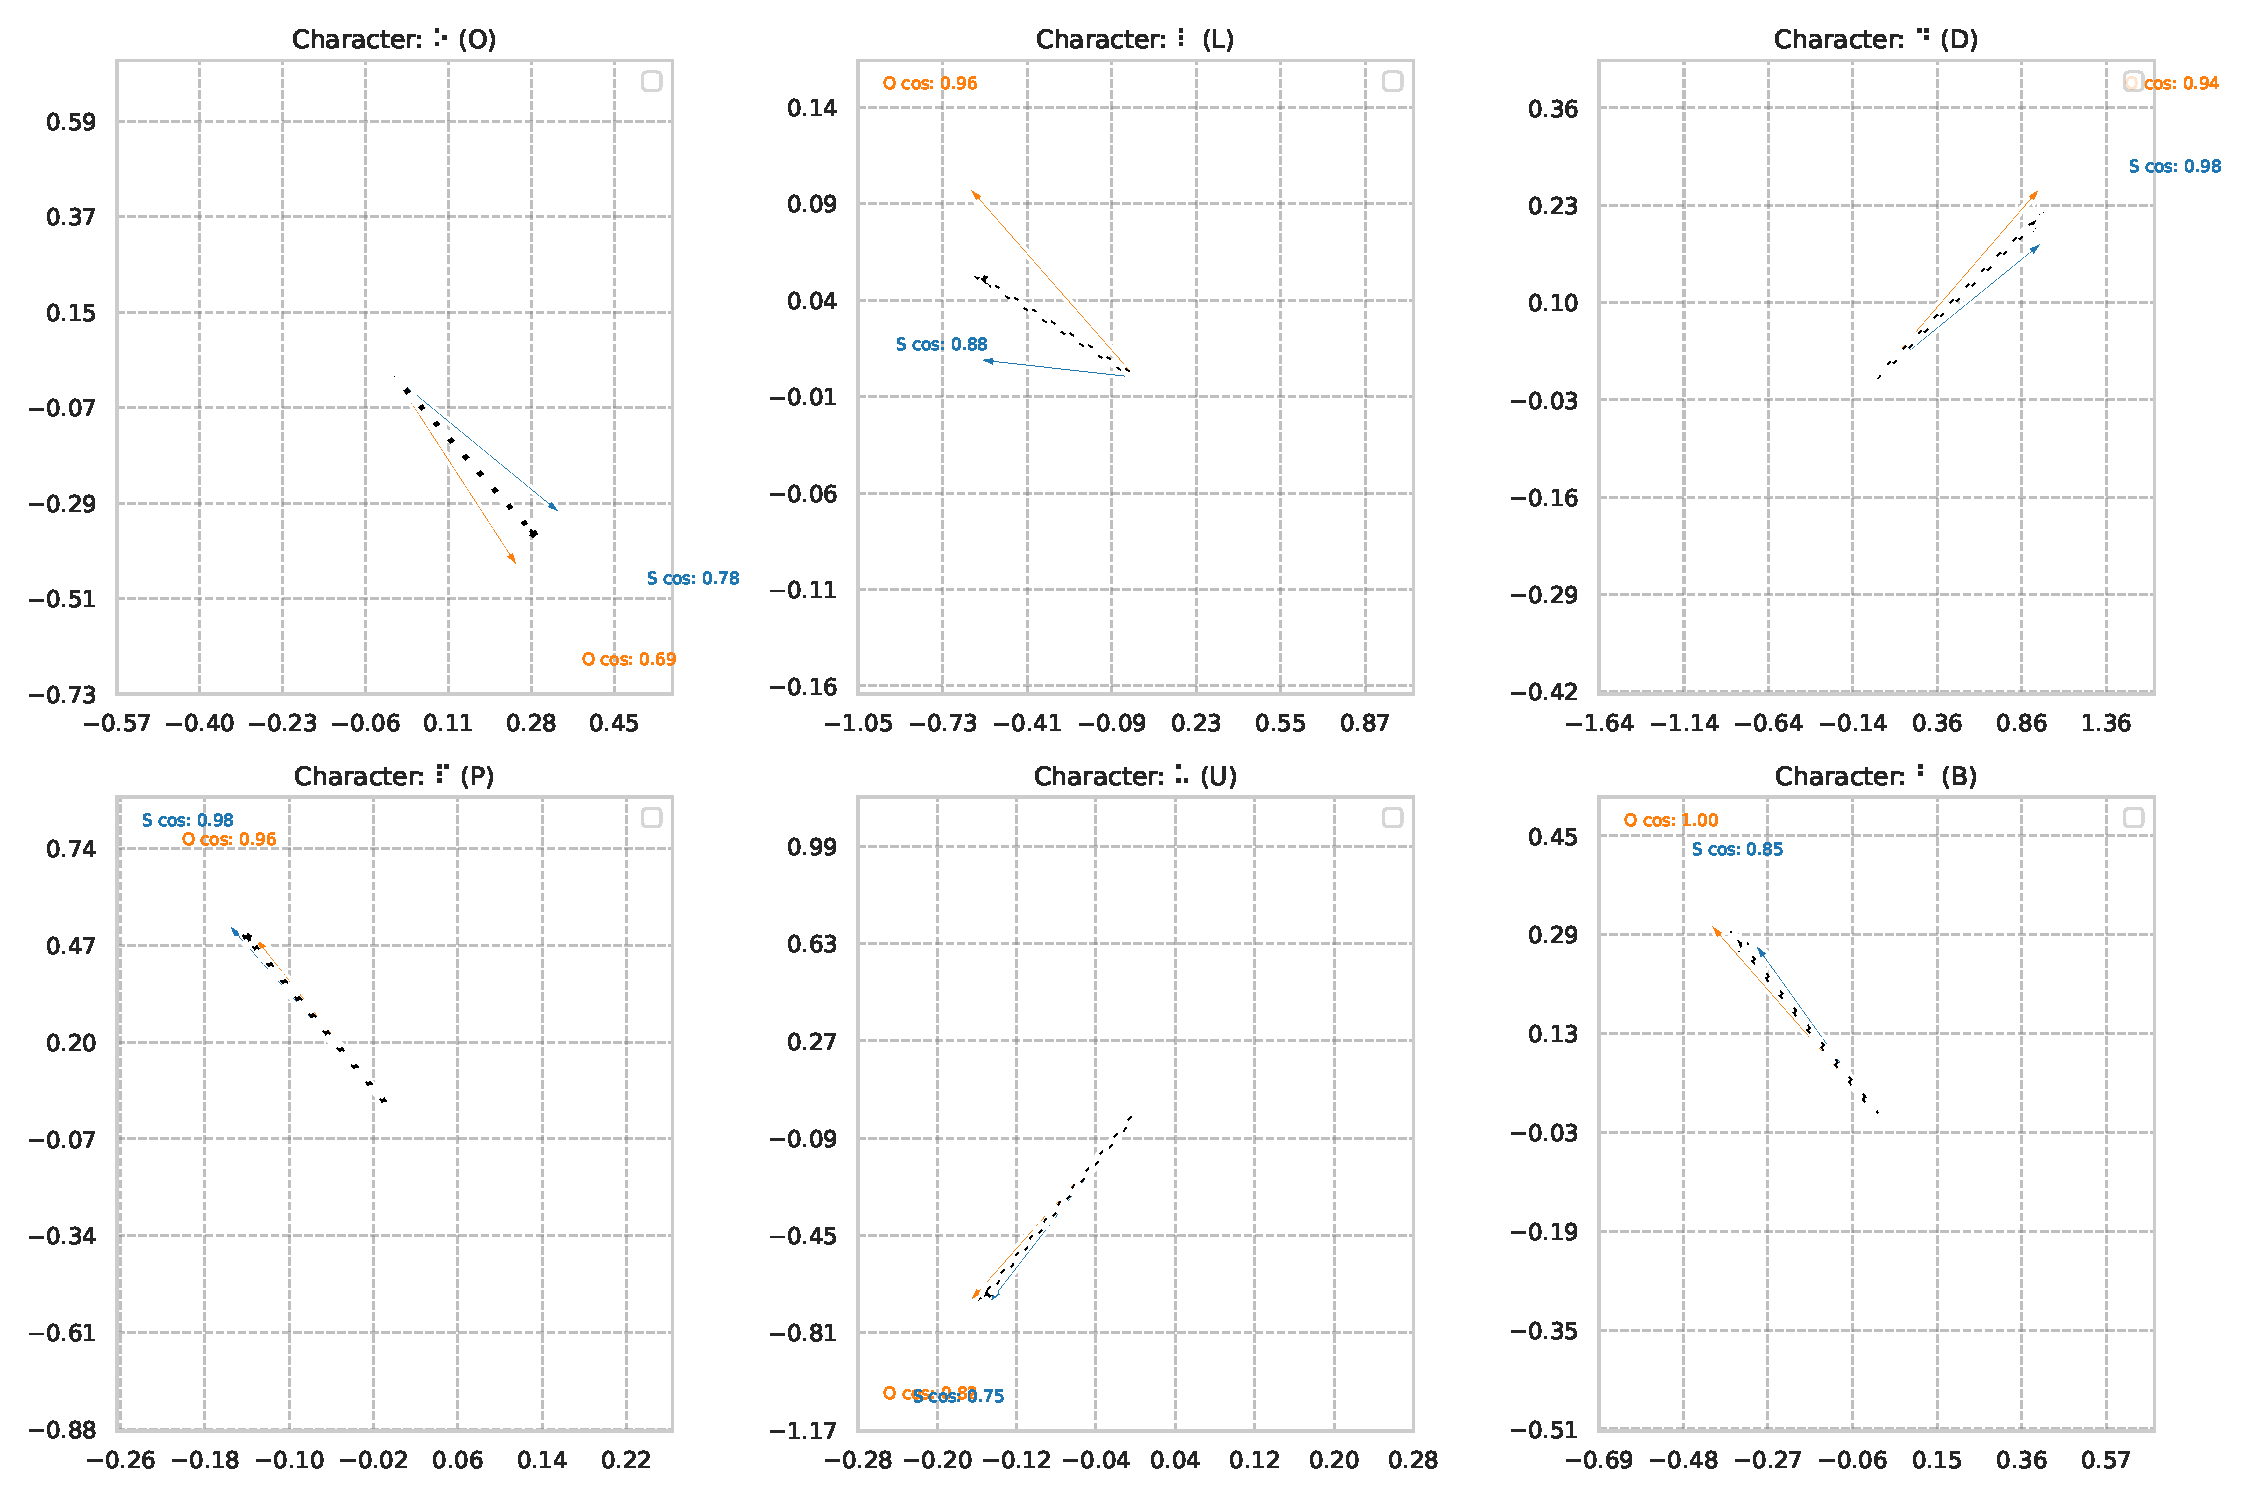
\includegraphics[width=\linewidth]{src/pictures/Study2Data_Experiment/Vectors_study2.pdf}
    \caption{Cosine Similariy for each Encoding.\\Plotted using a PCA dimensionality reduction.}
    \label{fig:cosSim_PCA_study2}
\end{figure}

The cosine similarity and \gls{pca} analysis, as shown in \autoref{fig:cosSim_PCA_study2}, indicate that despite noise reduction through \gls{pca}, the vectors align in a similar direction. The most noticeable differences were observed for the braille characters \braille{o}(O) and especially \braille{l}(L).
However, their cosine similarity scores are still rather similar with 0.69 for the \gls{ost} and 0.78 for \gls{seq} for the braille character \braille{o}(O).
For the Braille character \braille{l}(L), the cosine similarity is even smaller with 0.96 for \gls{ost} and 0.88 for \gls{seq}.
